% ======================================================================
% Scientific Reports — Supplementary Information, compiled as the single
% separate PDF the journal requires. First page carries the title and
% author list. Items are numbered S1, S2, ...; the article's labels are
% read through xr-hyper so that main-text equations, tables and figures
% can be cited from here. Build with .\build_SR.ps1 (which compiles the
% article and this file alternately until the cross-references settle).
% ======================================================================
\documentclass[12pt,a4paper]{article}

\newif\ifanon
\anonfalse

\newcommand{\SRexternaldoc}{main_SR}
\newcommand{\SRpdftitle}{Supplementary Information: A translatability verdict for cross-domain medical prediction that reports what a scarce cohort can adjudicate}
\newcommand{\SRrunninghead}{Supplementary Information}
% ============================================================
% Preamble — Scientific Reports build (main_SR.tex and
% supplementary_SR.tex share it).
% Journal guidance (https://www.nature.com/srep/author-instructions/
% submission-guidelines): single-column, unjustified text; Arabic page
% number in the footer; default Computer Modern fonts; numeric citations
% in square brackets in Nature style; line numbers recommended;
% equations cited as "equation (1)".
%
% The file that \input{}s this preamble must define \SRexternaldoc
% (the jobname of the companion document whose labels are read with
% xr-hyper: the article reads the supplement and vice versa) and
% \SRpdftitle.
% ============================================================

\usepackage[utf8]{inputenc}
\usepackage[T1]{fontenc}
\usepackage[english]{babel}
\usepackage{lmodern}
\usepackage{microtype}

\usepackage[a4paper,top=25mm,bottom=25mm,left=25mm,right=25mm]{geometry}
\usepackage{setspace}
\onehalfspacing
% Unjustified single-column text, as the journal asks of revised files.
\usepackage[document]{ragged2e}
\setlength{\RaggedRightParindent}{\parindent}

% Line numbers on every page of the article (journal recommendation).
\usepackage[mathlines]{lineno}
\linenumbers
\renewcommand\linenumberfont{\normalfont\tiny\color{gray}}

\usepackage{amsmath,amssymb,bm,mathtools}
\usepackage{graphicx}
\graphicspath{{figures/casegrid_1600/}{figures/}}
\usepackage{float}
\usepackage{placeins}
\usepackage{subcaption}
\usepackage[labelfont=bf,font=small]{caption}

\setcounter{topnumber}{3}
\setcounter{bottomnumber}{2}
\setcounter{totalnumber}{4}
\renewcommand{\topfraction}{0.9}
\renewcommand{\bottomfraction}{0.7}
\renewcommand{\textfraction}{0.1}
\renewcommand{\floatpagefraction}{0.5}

% Inside table floats the size ladder is the 10 pt one (normal 10,
% small 9, footnote 8, script 7) so that no table overruns one page.
\usepackage{etoolbox}
\newcommand{\tablesizes}{%
  \renewcommand{\normalsize}{\fontsize{10}{12}\selectfont}%
  \renewcommand{\small}{\fontsize{9}{10.5}\selectfont}%
  \renewcommand{\footnotesize}{\fontsize{8}{9.5}\selectfont}%
  \renewcommand{\scriptsize}{\fontsize{7}{8}\selectfont}%
  \normalsize}
% Inside floats the ragged2e paragraph indent is dropped, otherwise a
% \resizebox{\linewidth} table starts an indented paragraph and overruns
% the text block by exactly \parindent.
\AtBeginEnvironment{table}{\tablesizes\setlength{\parindent}{0pt}%
  \setlength{\RaggedRightParindent}{0pt}\setlength{\CenteringParindent}{0pt}}
\AtBeginEnvironment{figure}{\setlength{\parindent}{0pt}%
  \setlength{\RaggedRightParindent}{0pt}\setlength{\CenteringParindent}{0pt}}

\usepackage{booktabs,multirow,makecell,longtable,tabularx,array}
\newcolumntype{C}[1]{>{\centering\arraybackslash}p{#1}}
\newcolumntype{L}[1]{>{\raggedright\arraybackslash}p{#1}}

\usepackage[dvipsnames,table]{xcolor}
\definecolor{linkblue}{RGB}{0,70,140}

% Cross-document references: the article cites Supplementary items and
% the Supplementary Information cites main-text equations, tables and
% figures. xr-hyper must precede hyperref.
\usepackage{xr-hyper}
% [nocite]: import labels only, not the other document's \bibcite
% entries (each document carries its own numbered reference list).
\externaldocument[][nocite]{\SRexternaldoc}

\usepackage[colorlinks,linkcolor=linkblue,citecolor=linkblue,urlcolor=linkblue,
  pdftitle={\SRpdftitle}]{hyperref}
\usepackage{xurl}
\usepackage[capitalise,noabbrev]{cleveref}
\crefformat{equation}{equation~(#2#1#3)}
\Crefformat{equation}{Equation~(#2#1#3)}
% Supplementary items are numbered S1, S2, ... and cited as
% "Supplementary Fig. S1" / "Supplementary Table S1" (journal style).
\crefname{suppfigure}{Supplementary Fig.}{Supplementary Figs.}
\Crefname{suppfigure}{Supplementary Fig.}{Supplementary Figs.}
\crefname{supptable}{Supplementary Table}{Supplementary Tables}
\Crefname{supptable}{Supplementary Table}{Supplementary Tables}

% Numeric citations in square brackets, Nature reference style.
\usepackage[numbers,sort&compress,square]{natbib}

\usepackage{fancyhdr}
\pagestyle{fancy}
\fancyhf{}
\fancyhead[L]{\small\textit{\SRrunninghead}}
\fancyfoot[C]{\small\thepage}
\renewcommand{\headrulewidth}{0.4pt}

\newcommand{\auroc}{\text{AUROC}}
\newcommand{\auprc}{\text{AUPRC}}
\newcommand{\fuzzyarc}{\textsc{FuzzyArcLoss}}
\newcommand{\abmil}{\textsc{ABMIL}}
\newcommand{\lchai}{\textsc{LCHAI}}
\newcommand{\ctranspath}{\textsc{CTransPath}}
\newcommand{\fcmil}{\textsc{FC-MIL}}
\newcommand{\piabmil}{\textsc{PI-ABMIL}}
\newcommand{\xgb}{\textsc{XGBoost}}

\DeclareMathOperator{\softmax}{softmax}
\newcommand{\sigmoid}{\sigma}

% Partial information decomposition (Williams & Beer atoms).
\newcommand{\pid}{\textsc{PID}}
\newcommand{\Ired}{\mathcal{R}}          % redundant information
\newcommand{\Iuni}[1]{\mathcal{U}_{#1}}  % unique information of source #1
\newcommand{\Isyn}{\mathcal{S}}          % synergistic information

% Uniform-size case-study panel: fixed box, image scaled to fit.
\newlength{\casepanelht}\setlength{\casepanelht}{4.4cm}
\newcommand{\casepanel}[1]{%
  \begin{minipage}[c][\casepanelht][c]{\linewidth}%
    \centering
    \includegraphics[width=\linewidth,height=\casepanelht,keepaspectratio]{#1}%
  \end{minipage}}

\ifanon\hypersetup{pdfauthor={}}\else
\hypersetup{pdfauthor={Servio F. Lima Reina, Servio R. Lima Idrobo, Doménica N. López García, Luis Terán}}\fi

\begin{document}
\thispagestyle{fancy}

\begin{center}
{\Large\bfseries Supplementary Information}\\[2ex]
{\large A translatability verdict for cross-domain medical prediction that
reports what a scarce cohort can adjudicate}\\[2ex]
\ifanon
Authors withheld for double-anonymised peer review\\[2ex]
\else
Servio F.~Lima Reina\textsuperscript{1,*}, Servio R.~Lima
Idrobo\textsuperscript{1}, Dom\'enica N.~L\'opez Garc\'ia\textsuperscript{1}
and Luis Ter\'an\textsuperscript{2}\\[1ex]
{\small \textsuperscript{1}GPTfy Medical, Guayaquil, Ecuador;
\textsuperscript{2}Lucerne University of Applied Sciences and Arts (HSLU),
Lucerne, Switzerland.
\textsuperscript{*}Correspondence: \href{mailto:slima@gptfy.biz}{slima@gptfy.biz}}\\[2ex]
\fi
\end{center}

% ======================================================================
% Supplementary Information — Scientific Reports build. Compiled as a
% separate single PDF by supplementary_SR.tex (which supplies the
% title-and-author first page the journal requires) and \input here.
% Everything that is not one of the seven main display items is
% Supplementary Information: figures, then tables, then notes.
%
% Numbering and cross-referencing: items are numbered S1, S2, ... as the
% journal asks, and \crefalias makes every label defined from here on
% resolve as "Supplementary Fig. SN" / "Supplementary Table SN" wherever it
% is cited, including from the article (which reads this file's labels
% through xr-hyper). Main-text labels are read the other way round.
% ======================================================================
\setcounter{figure}{0}
\setcounter{table}{0}
\renewcommand{\thefigure}{S\arabic{figure}}
\renewcommand{\thetable}{S\arabic{table}}
\renewcommand{\figurename}{Supplementary Fig.}
\renewcommand{\tablename}{Supplementary Table}
\crefalias{figure}{suppfigure}
\crefalias{table}{supptable}

\noindent\textbf{Contents.} Supplementary Figs.~S1--S10; Supplementary
Tables~S1--S19; Supplementary Notes~1--5 (extended protocol for the two
additional modalities, including the glioma pilot and the MGMT
full-power null; position against the published mutation-prediction
literature; relation to prior information-decomposition work; levels
of analysis and the scope of a verdict; extended limitations). Equation, figure and table numbers
without the S prefix refer to the main article.

\clearpage
% ======================================================================
\section*{Supplementary Figures}
% ======================================================================

% --- Supplementary Fig. 1: the LUAD signal tree (demoted from the main
% text: every LUAD regime read is directional and unadjudicated) ---
\begin{figure}[htbp]
  \centering
  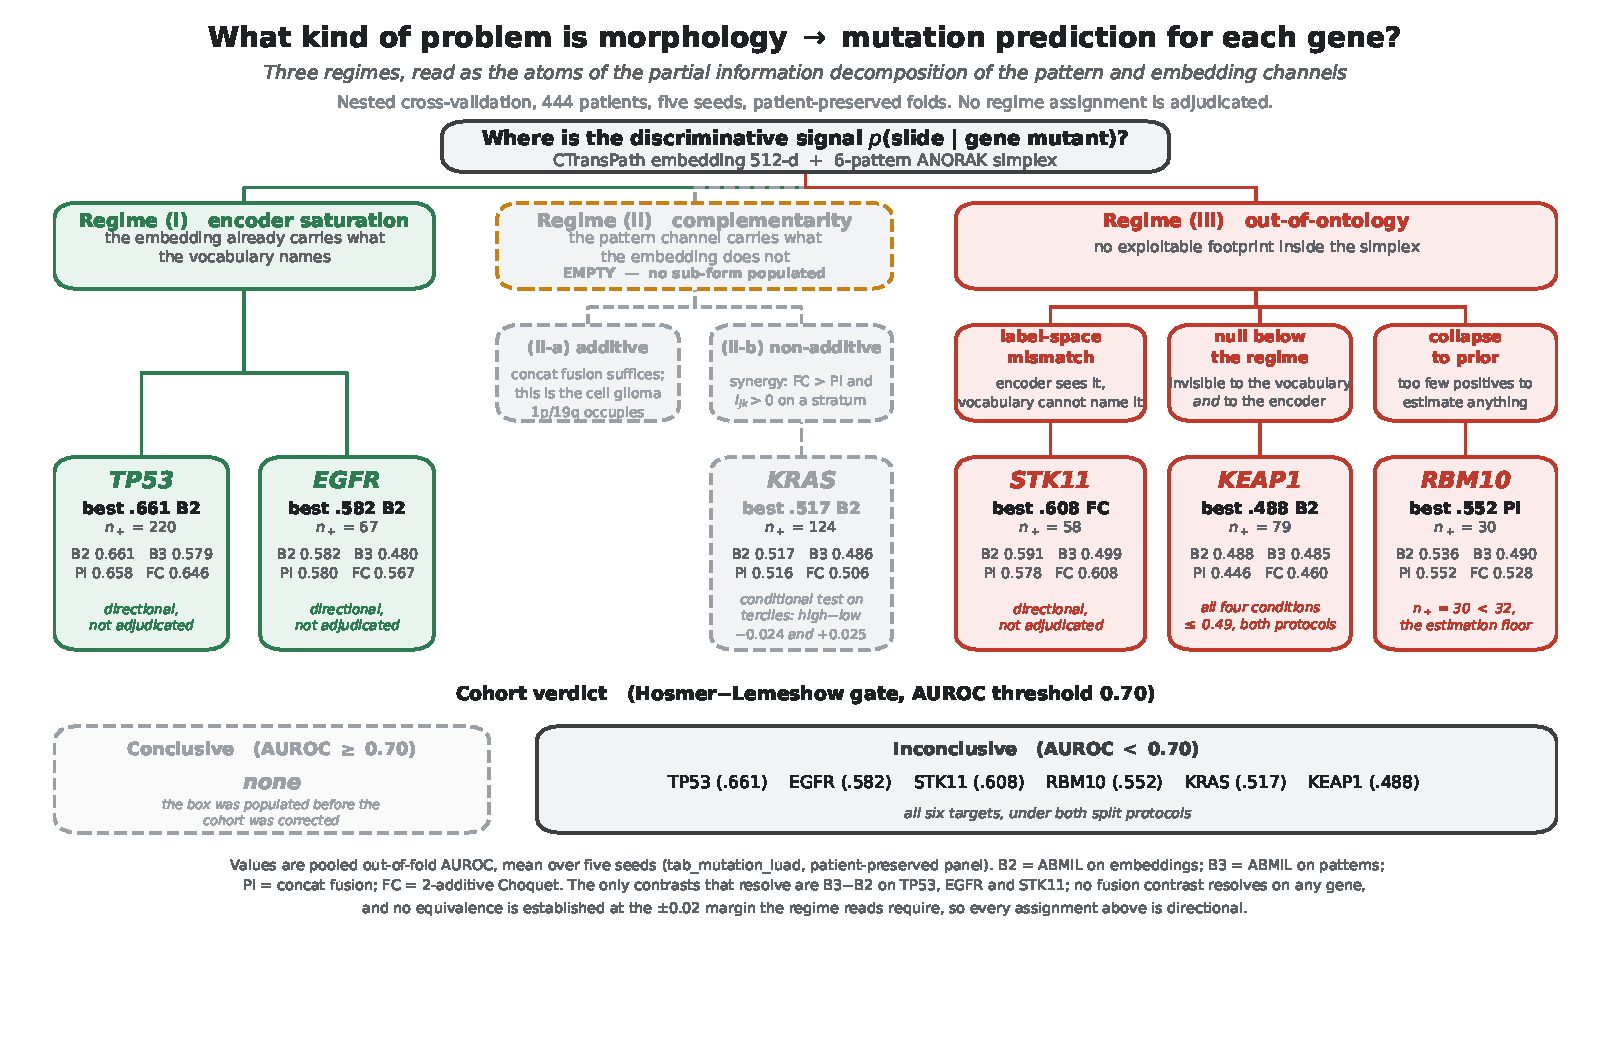
\includegraphics[width=\linewidth]{signal_tree}
  \caption{\textbf{Where the mutation signal lives, gene by gene: the
  three regimes of \cref{eq:pid} as a decision tree over the four
  training conditions.} Each read is directional: it follows the sign of
  the deciding contrast, and none is established, because no fusion
  contrast excludes zero or falls inside the $\pm0.02$ equivalence
  margin (Table~2). Regime~(i), encoder saturation (\textit{TP53},
  \textit{EGFR}): the embedding already carries what the vocabulary
  names. Regime~(ii), complementarity: its additive sub-form (ii-a) is
  empty in LUAD, and its non-additive sub-form (ii-b), tested on
  \textit{KRAS} by the conditional co-activation contrast, returns
  empty (\cref{tab:kras_coactivation}). Regime~(iii), out-of-ontology
  (\textit{STK11}, \textit{KEAP1}, \textit{RBM10}): the vocabulary
  converts into no gain, for three different reasons that one
  Inconclusive label conflates---label-space mismatch, modality ceiling
  and collapse to prior. The cohort size each read would need for
  confirmation is in \cref{tab:design_power}.}
  \label{fig:signal_tree}
\end{figure}

% --- Supplementary Fig. 2: the KRAS morphological proxy (demoted from
% the main text: the conditional synergy test it illustrates is a null) ---
\begin{figure}[htbp]
  \centering
  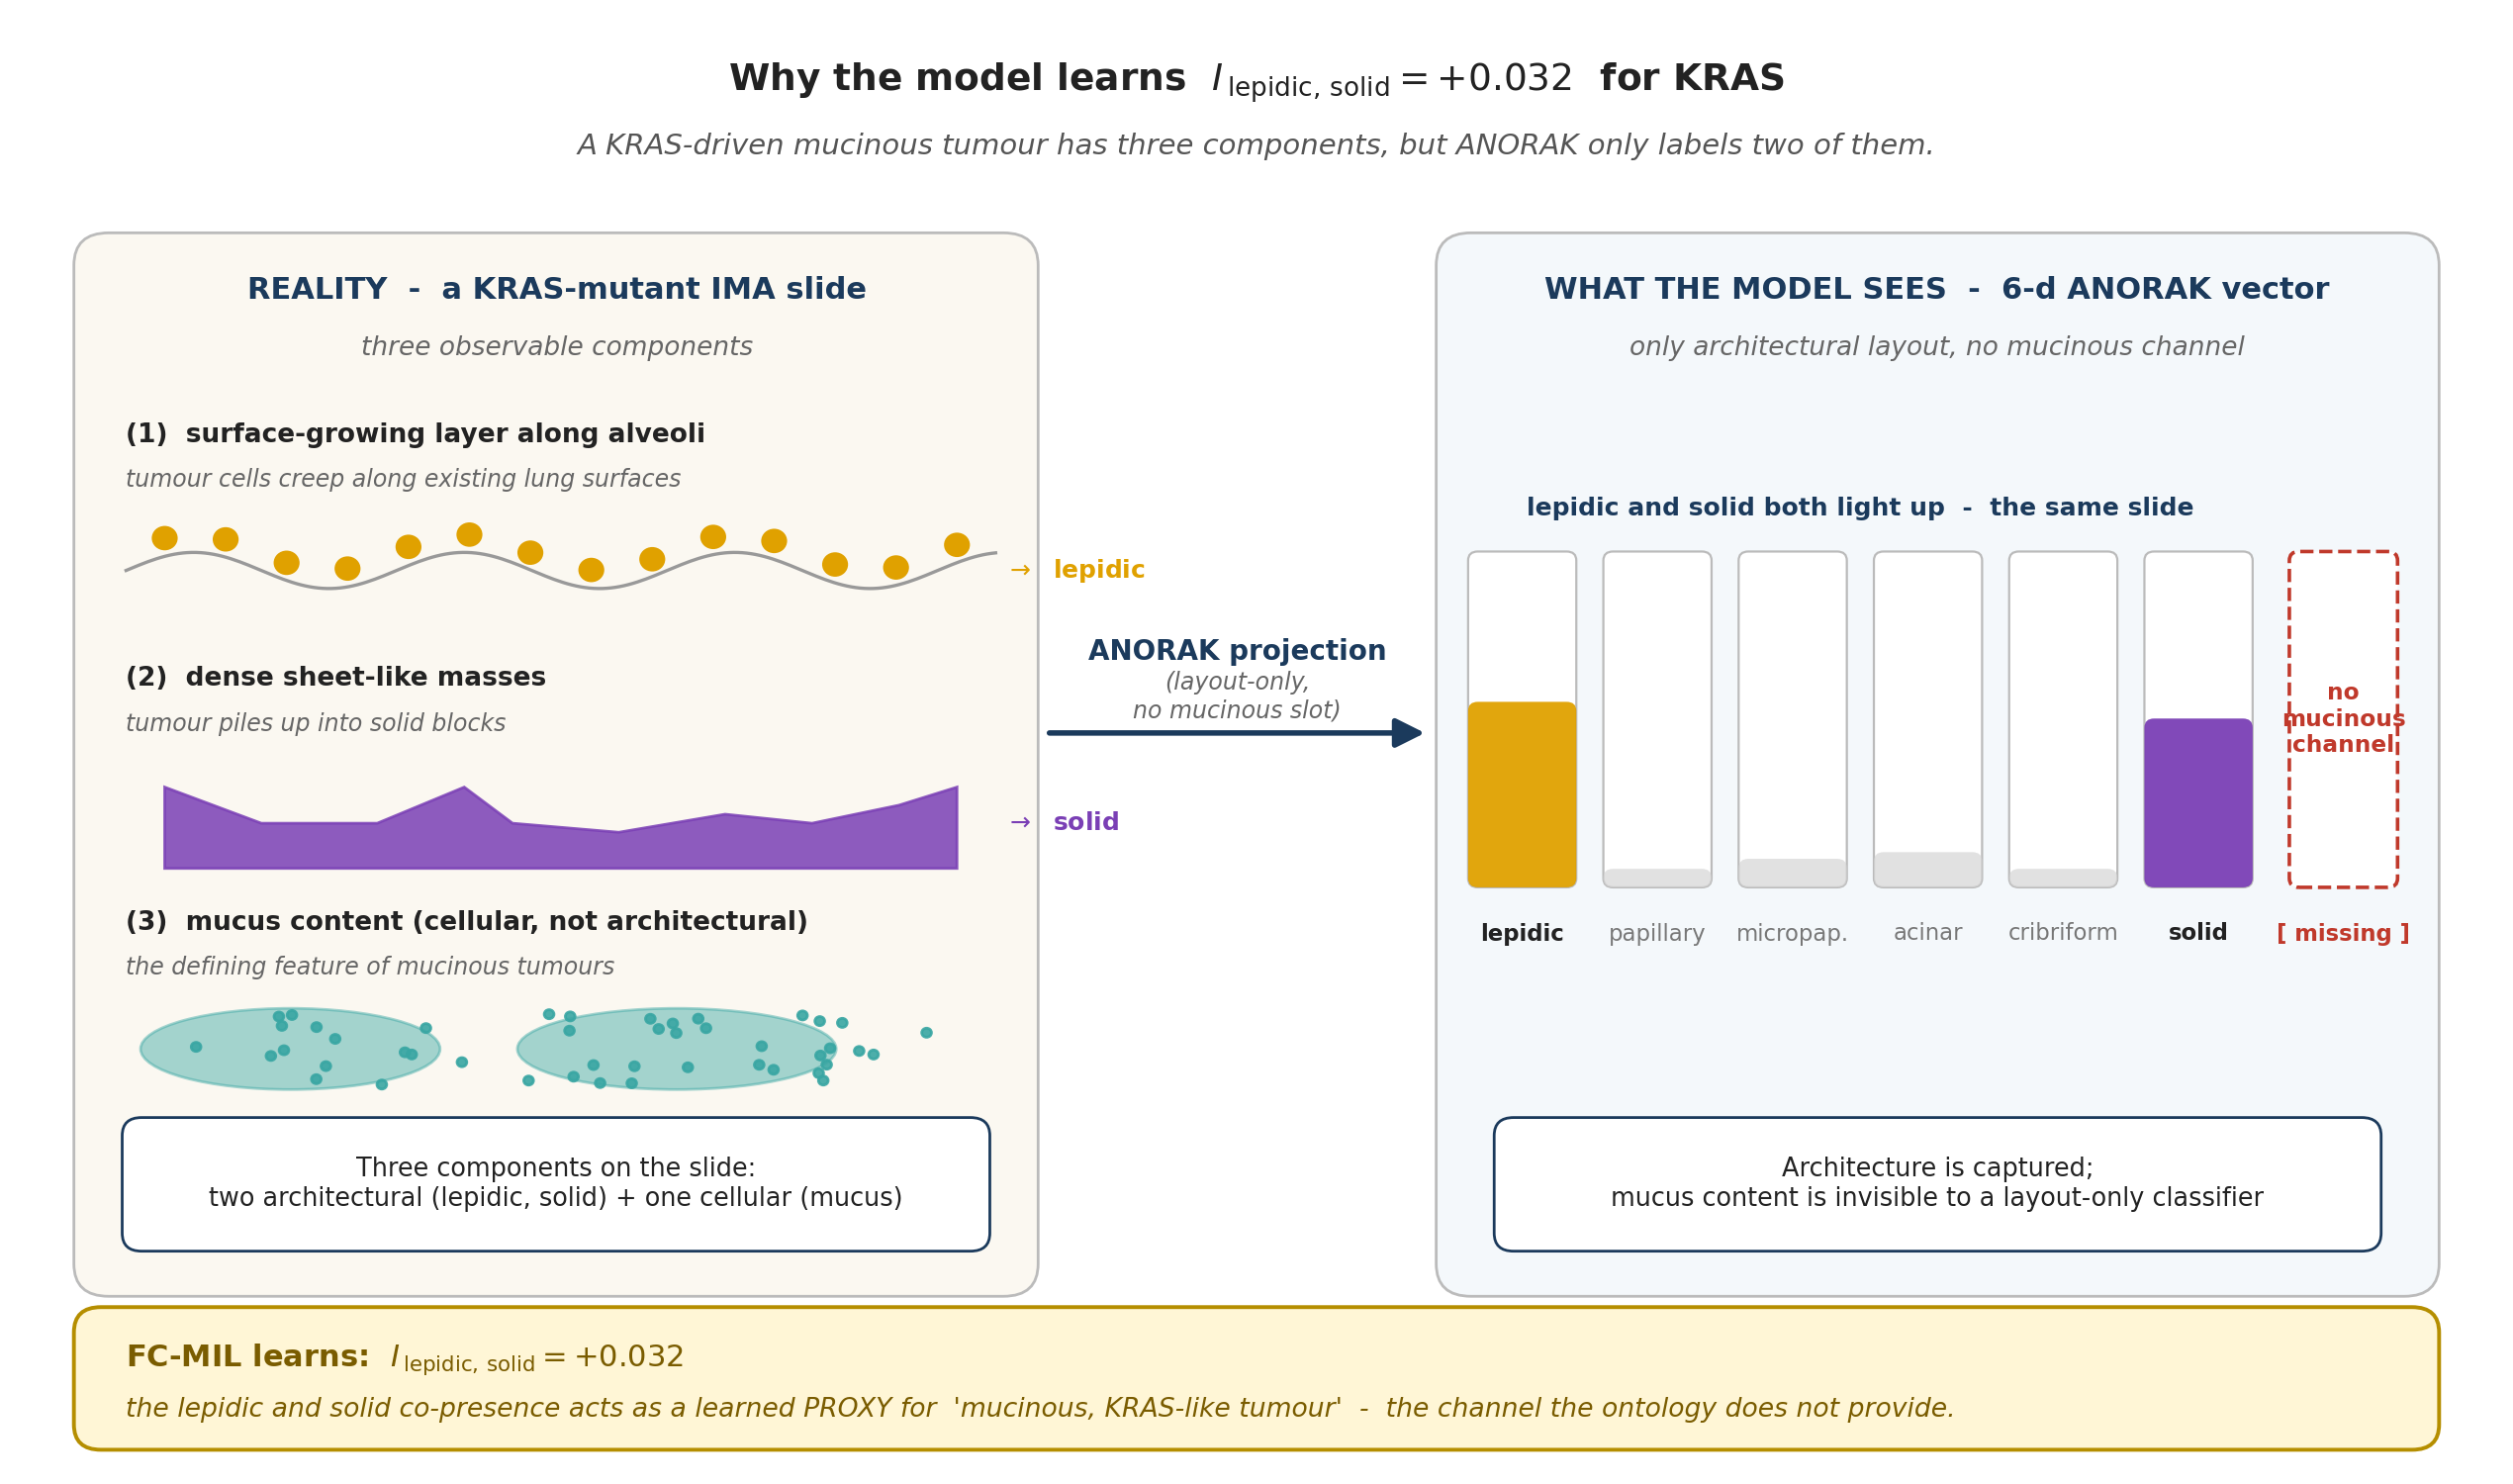
\includegraphics[width=\linewidth]{kras_lepidic_solid_proxy}
  \caption{\textbf{The pattern pair the Choquet head selects for KRAS,
  and the textbook morphology it stands for.} Left, the three
  components of a KRAS-driven invasive mucinous adenocarcinoma slide
  (a tumour-cell layer growing along alveoli, dense sheet-like masses,
  extracellular mucin). Right, what the $6$-d ANORAK vector retains of
  it: lepidic and solid light up together, and the mucin has no
  pattern. The positive interaction
  $I(\text{lepidic}\!\times\!\text{solid})\!=\!{+}0.032$ the
  $2$-additive measure learns on \textit{KRAS} is the aggregator paying
  for that co-occurrence, the histological proxy for invasive mucinous
  adenocarcinoma, the KRAS-enriched
  subtype.\cite{rekhtman2013krassolid} The index is a
  parameter of the fitted measure shared by every slide; whether it buys
  accuracy where the pair co-activates is the conditional test of
  \cref{tab:kras_coactivation}, which returns empty at this cohort size.
  The full Choquet read-out is \cref{fig:choquet_kras}.}
  \label{fig:kras_lepidic_solid_proxy}
\end{figure}

% --- Supplementary Fig. 3: the released per-slide tooling ---
\begin{figure}[htbp]
  \centering
  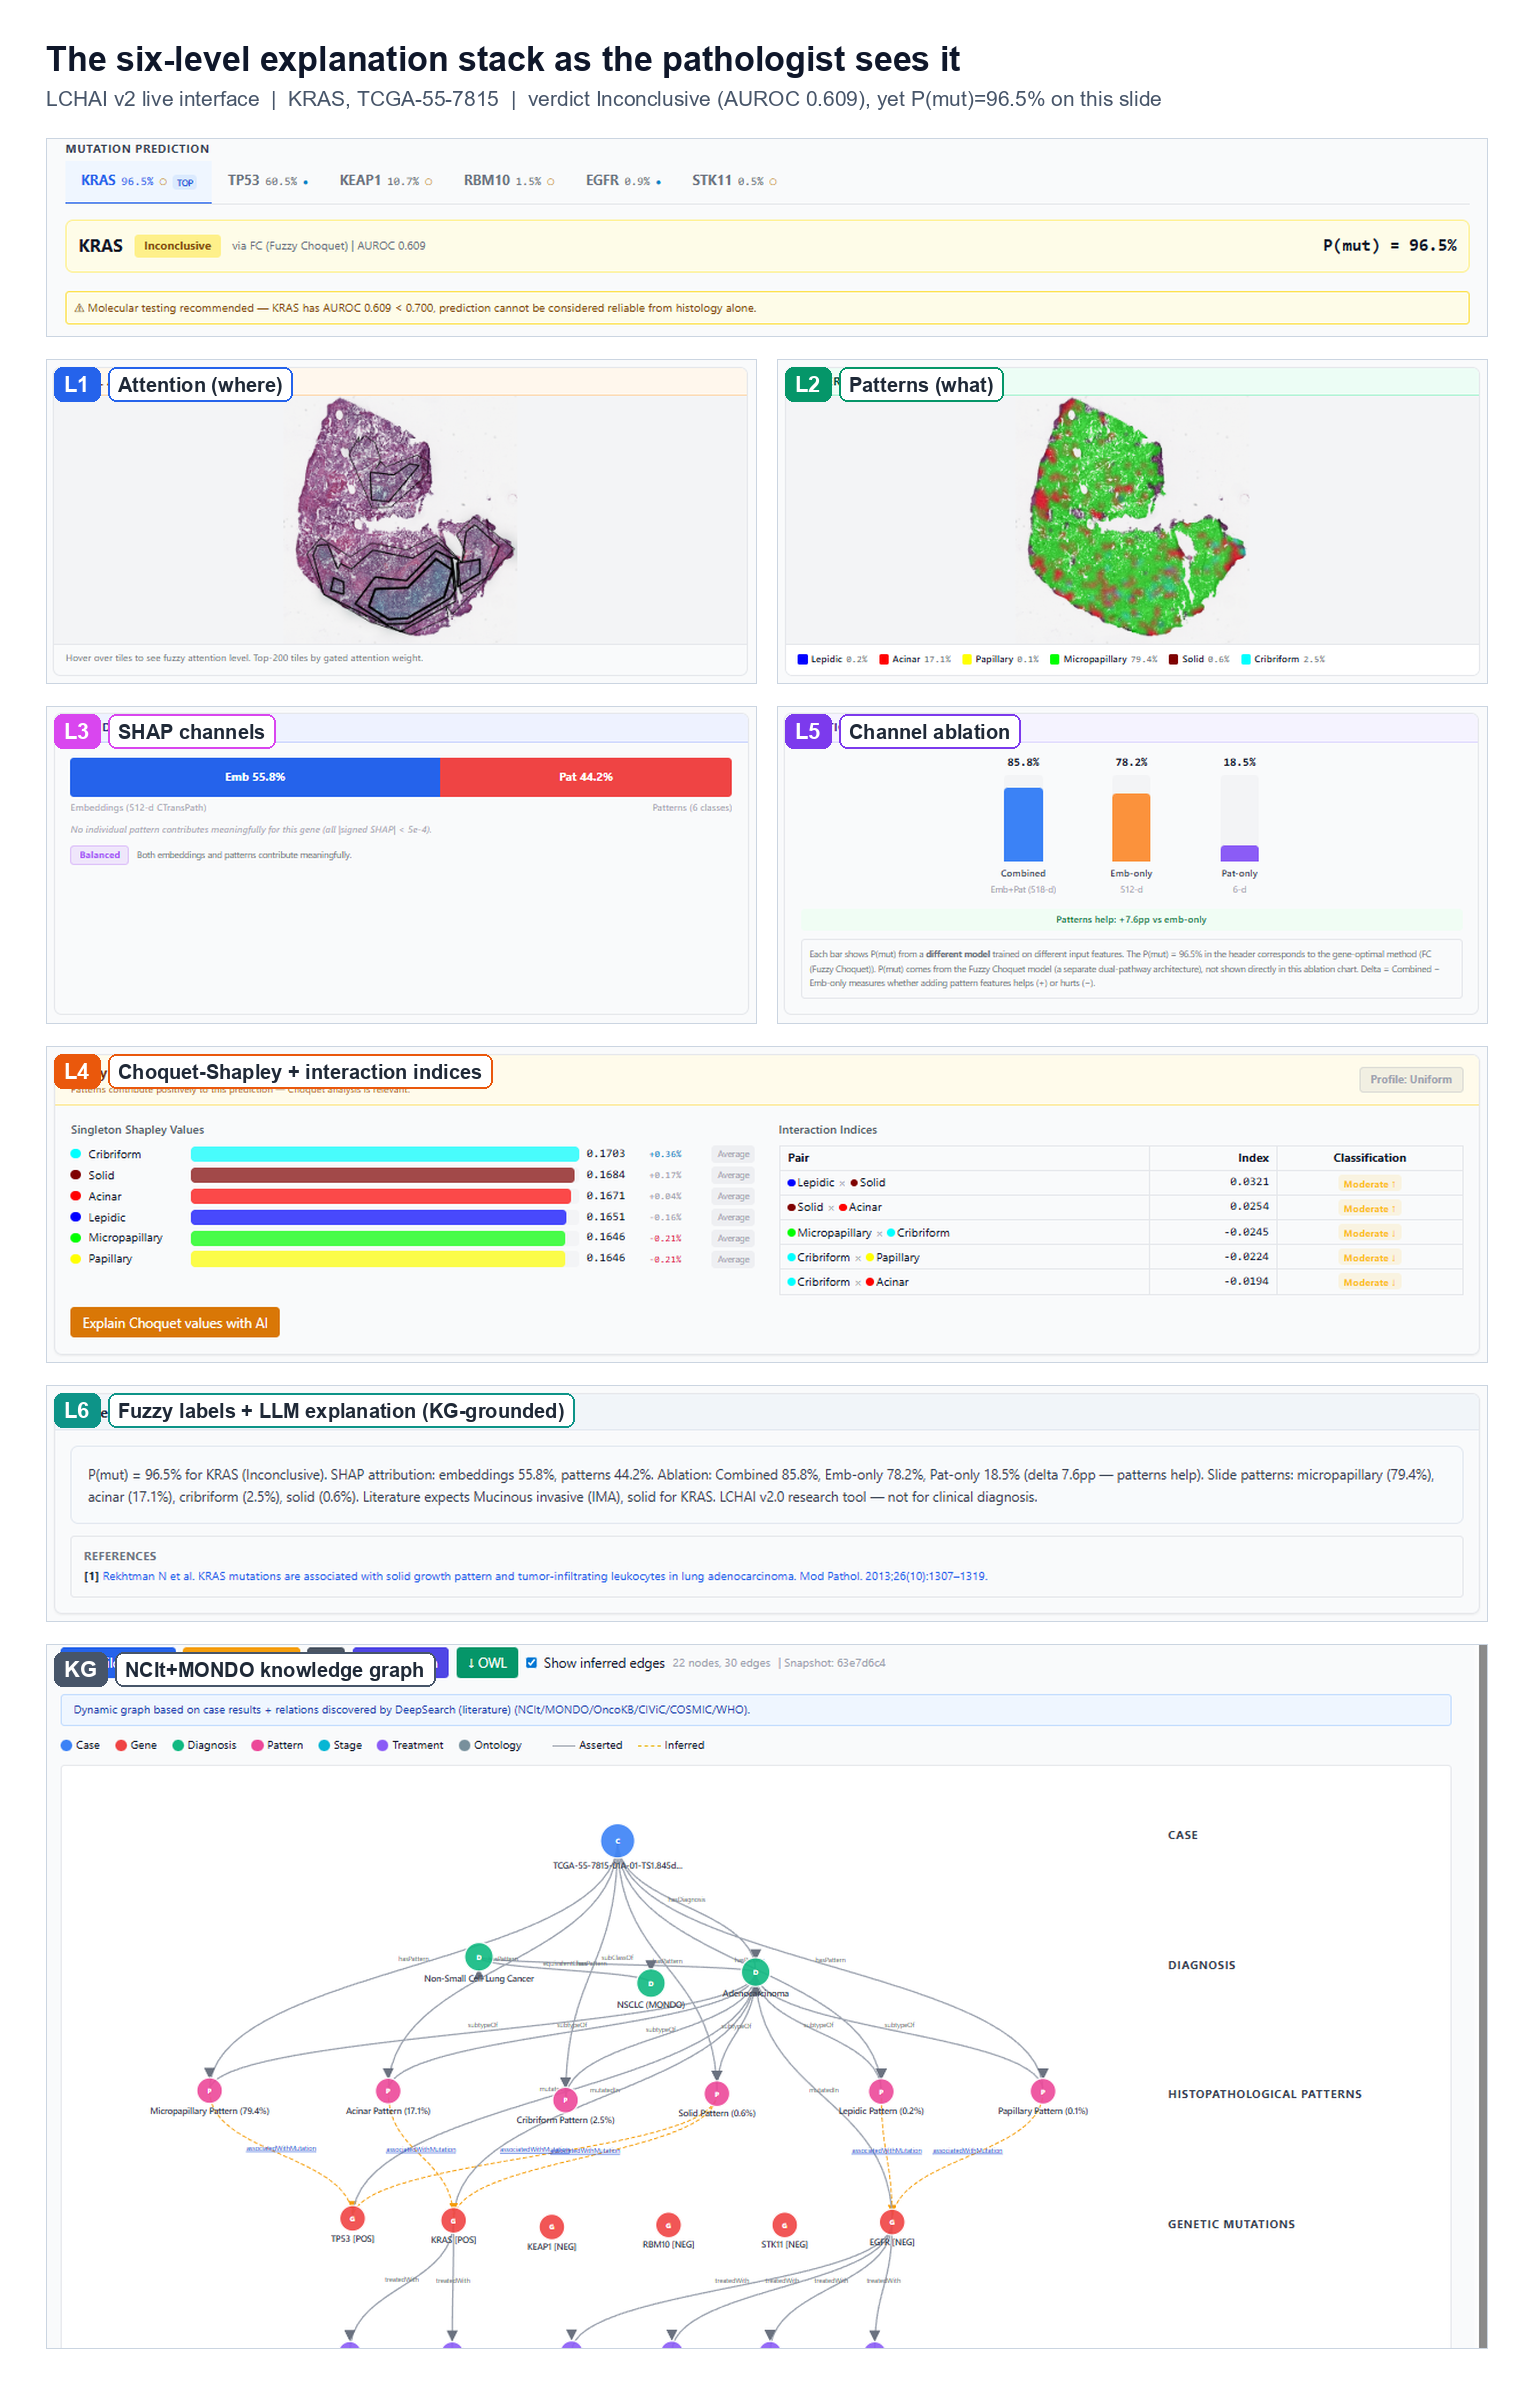
\includegraphics[width=\linewidth,height=0.68\textheight,keepaspectratio]{lchai_ui_six_levels}
  \caption{\textbf{The released per-slide tooling (\lchai{}~v2
  interface)}, for KRAS on TCGA-55-7815, a case whose cohort verdict is
  Inconclusive yet whose slide-level prediction is
  $P(\mathrm{mut})=0.965$. The top strip carries the population verdict
  and the slide-level prediction, with the molecular-testing flag raised
  whenever $\auroc<0.70$. The six read-outs are materialised from a
  single forward pass: \textbf{L1} ABMIL attention, \textbf{L2} pattern
  overlay, \textbf{L3} SHAP embedding/pattern split, \textbf{L4}
  Choquet--Shapley singleton values and pairwise interaction indices,
  \textbf{L5} channel ablation, and \textbf{L6} the fuzzy-label language
  output with its knowledge-graph-grounded references. The tooling is
  released as software and is not evaluated in this study (Methods). All
  imagery is from the public TCGA-LUAD cohort; the system is a research
  tool and is not for clinical diagnosis. The cohort \auroc{} printed in
  the strip ($0.609$) is the earlier single-split estimate served by the
  deployment at the time of capture (Supplementary Note~2) and differs
  from the nested cross-validation values of Table~1.}
  \label{fig:ui_stack}
\end{figure}

% --- Supplementary Fig. 4: glioma pipeline ---
\begin{figure}[htbp]
\centering
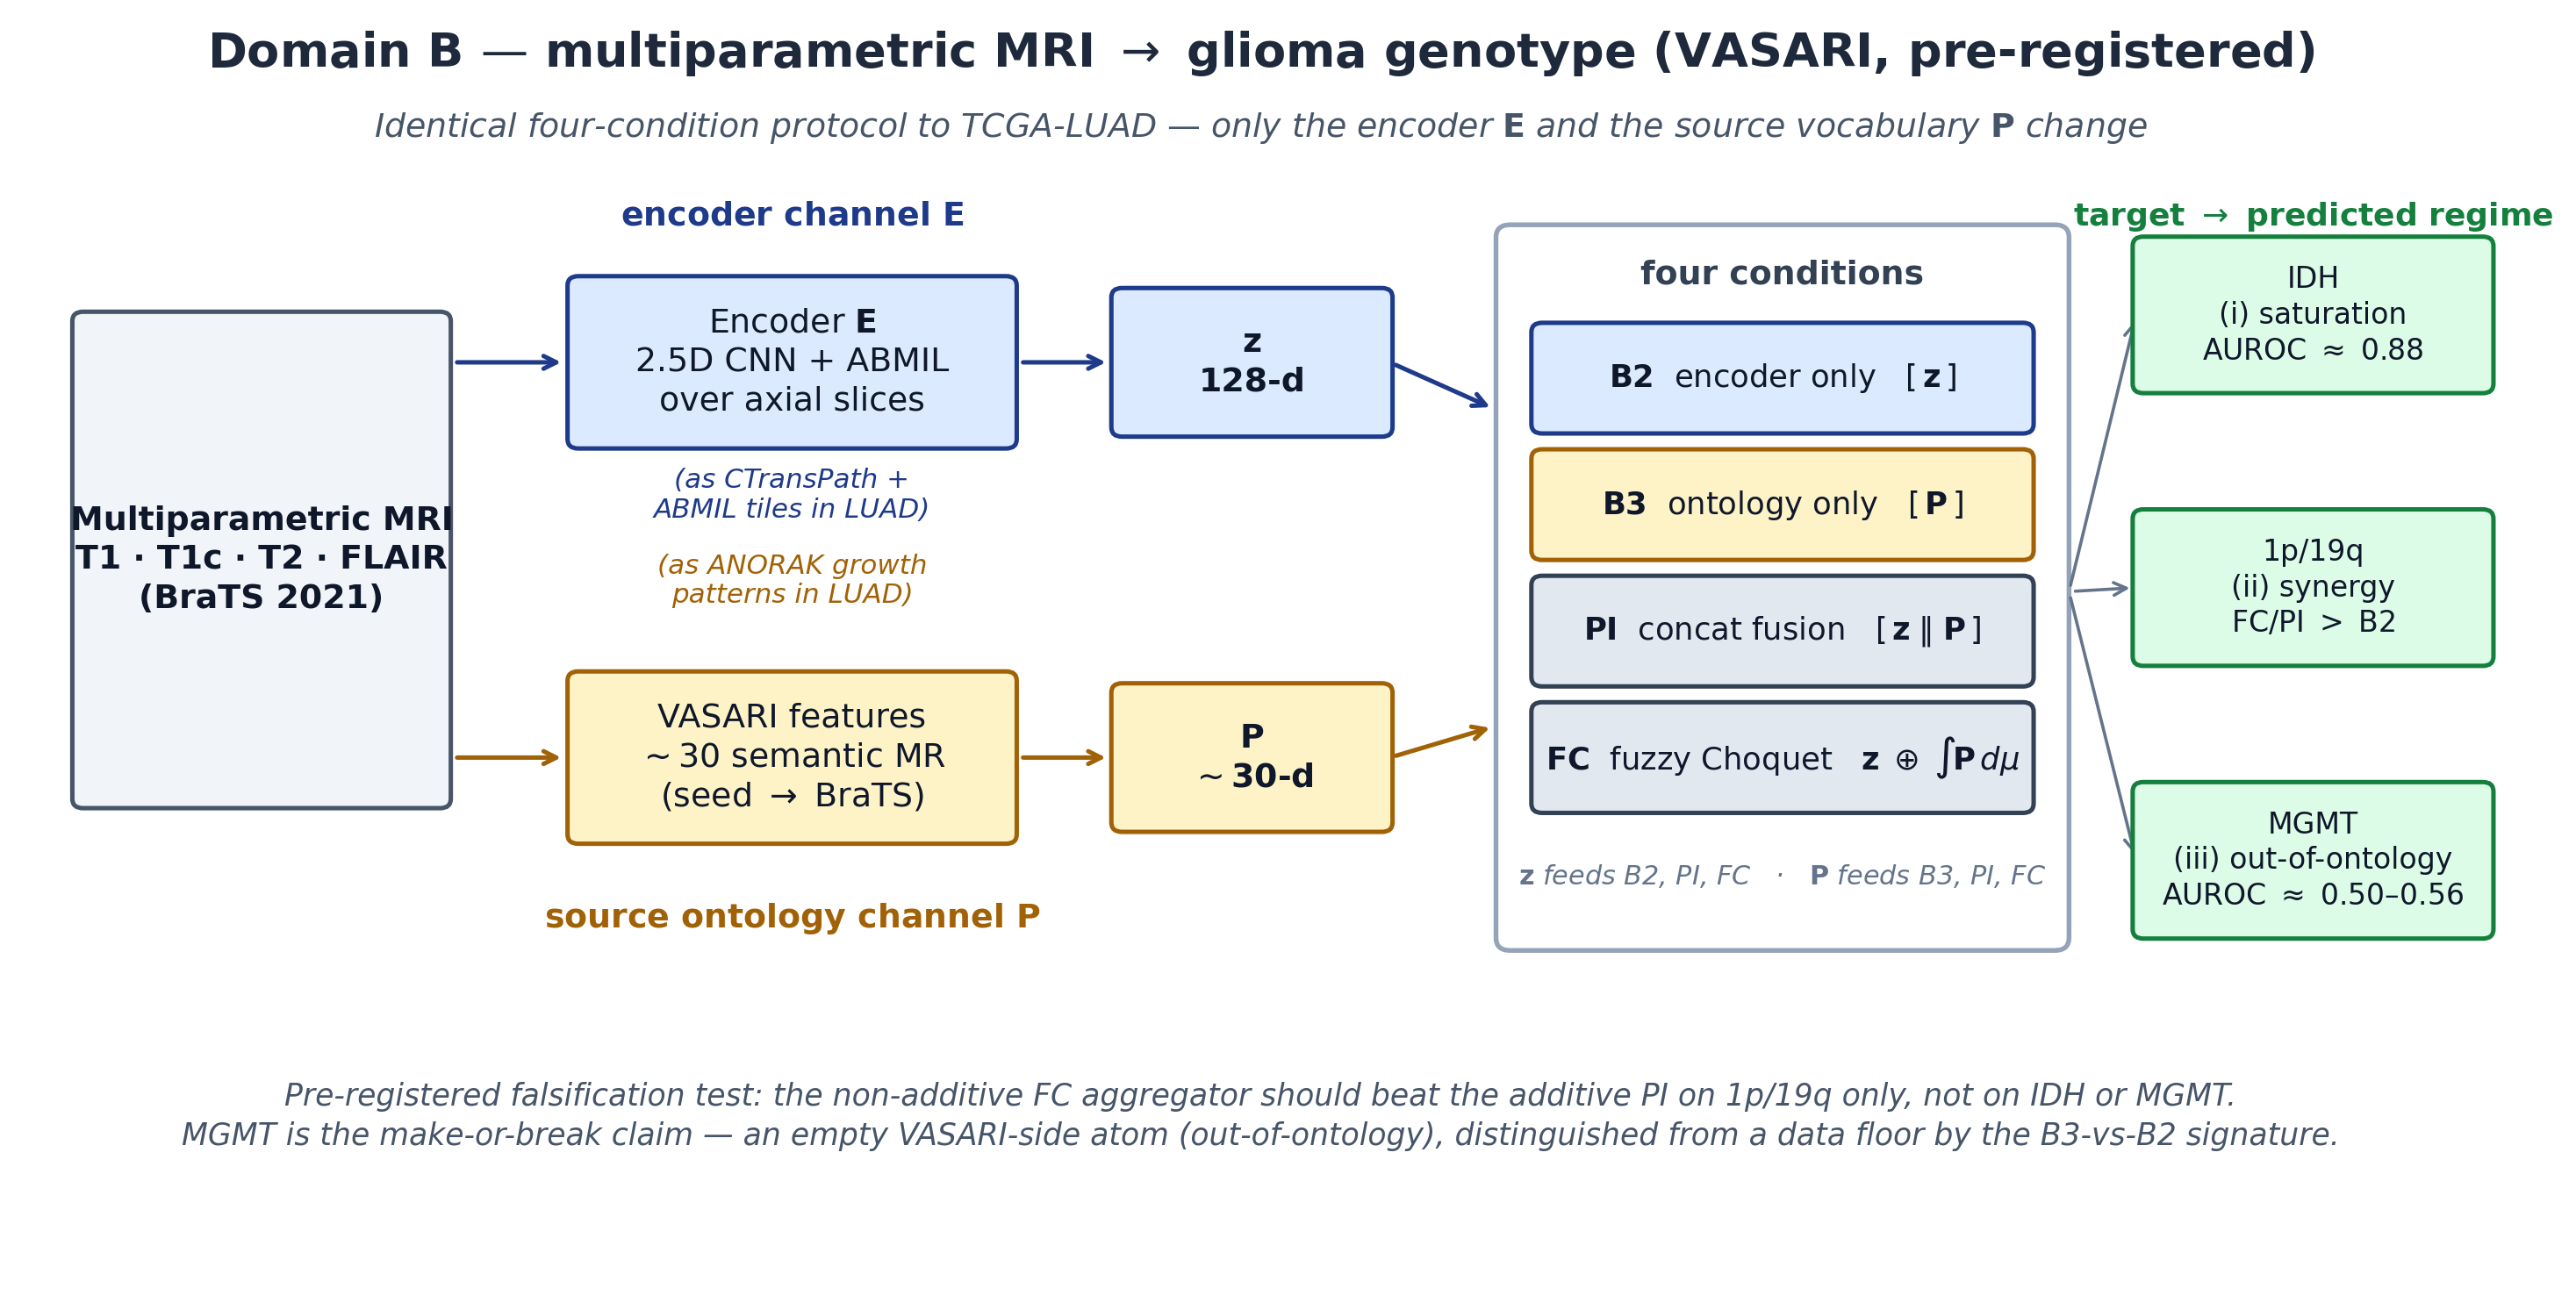
\includegraphics[width=\linewidth]{pipeline_glioma_domainB}
\caption{\textbf{The glioma MRI\,$\rightarrow$\,genotype pipeline as a
one-to-one transfer of the LUAD architecture.} An unconstrained learned
encoder $\mathbf{E}$---a 2.5D CNN with \abmil{} over axial MRI slices,
occupying the position \ctranspath{} with tile-level \abmil{} holds in
LUAD---and the expert source vocabulary $\mathbf{P}$---the VASARI semantic
MR features, expert-scored on the TCGA-LGG arm and propagated from the
annotated seed for the BraTS MGMT arm, occupying the position ANORAK growth
patterns hold in LUAD---feed
the same four conditions: B2 encoder only, B3 ontology only, PI concat
fusion and FC $2$-additive Choquet. Measured outcomes are in
\cref{tab:crossdomain_merged} (MGMT, full power) and
\cref{tab:glioma_domainb} (TCGA-LGG pilot).}
\label{fig:pipeline_glioma}
\end{figure}

% --- Supplementary Fig. 5: ECG pipeline ---
\begin{figure}[htbp]
\centering
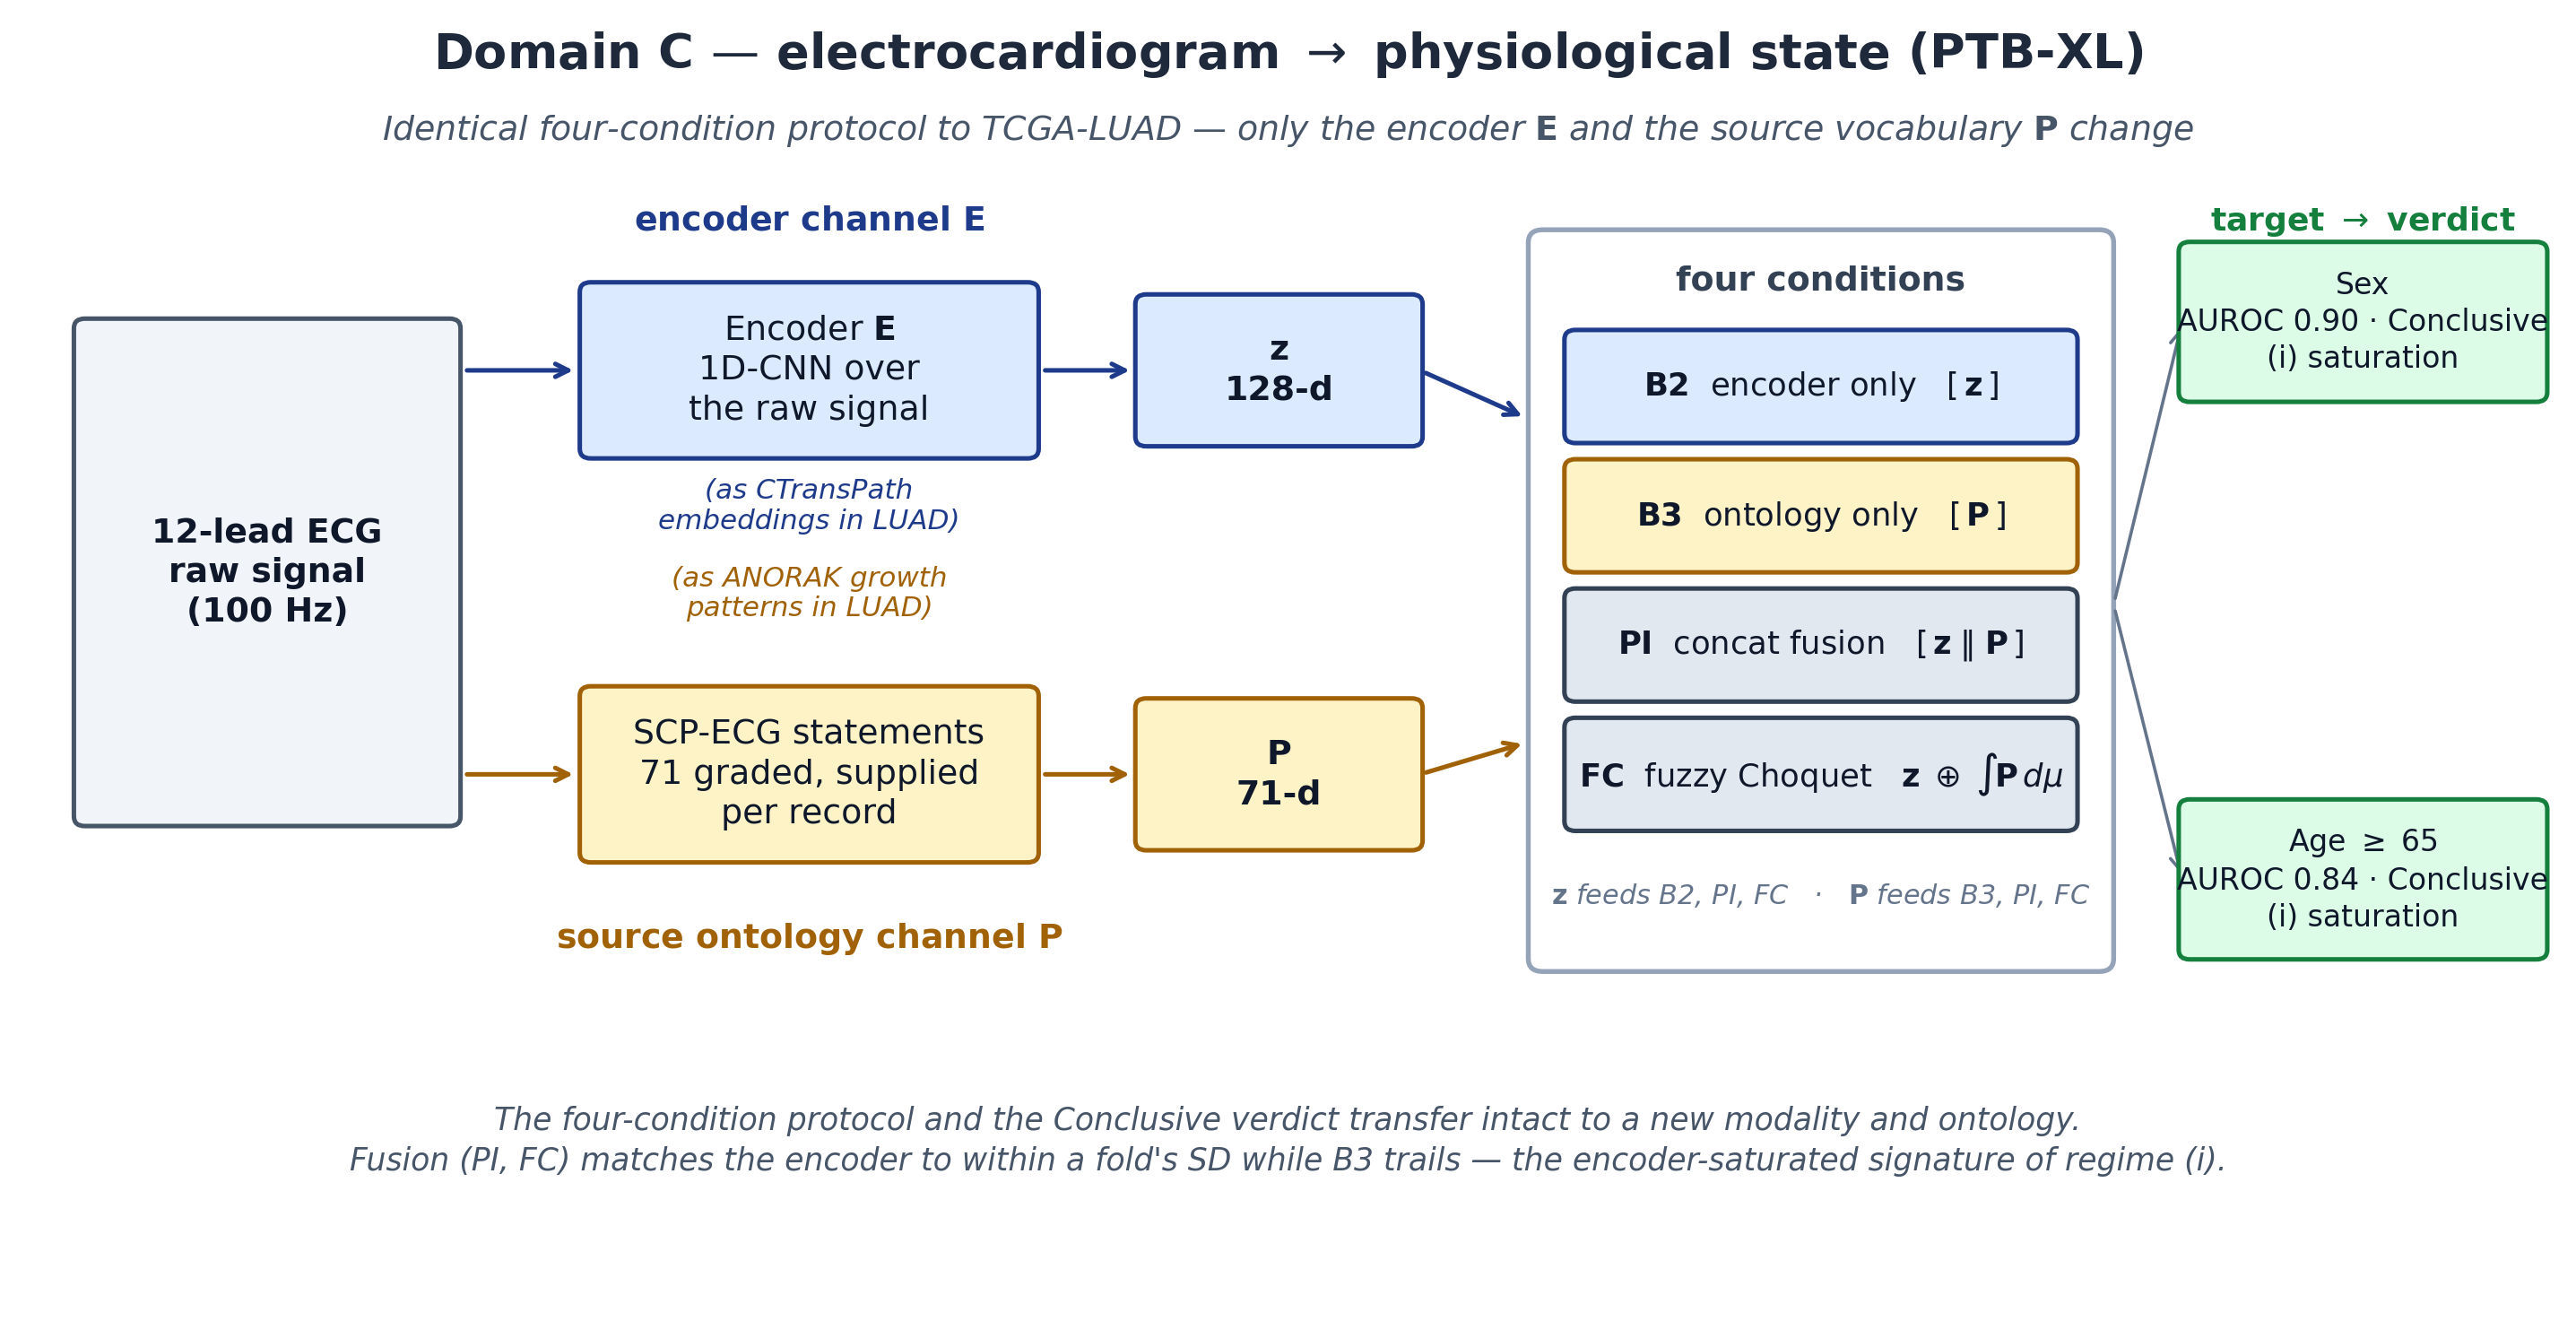
\includegraphics[width=\linewidth]{pipeline_ecg_domainC}
\caption{\textbf{The electrocardiogram\,$\rightarrow$\,physiological-state
pipeline running the identical four-condition protocol in a different
modality family.} The encoder $\mathbf{E}$---a 1D convolutional network
over the raw twelve-lead signal---and the source vocabulary
$\mathbf{P}$---the $71$ graded SCP-ECG statements---feed B2, B3, PI and FC
exactly as \ctranspath{} embeddings and ANORAK patterns do in LUAD. Both
targets are Conclusive and encoder-saturated: the fusion conditions match
the encoder to within a fold's standard deviation while the statement
channel alone trails.}
\label{fig:pipeline_ecg}
\end{figure}

% --- Supplementary Fig. 6 ---
\begin{figure}[htbp]
\centering
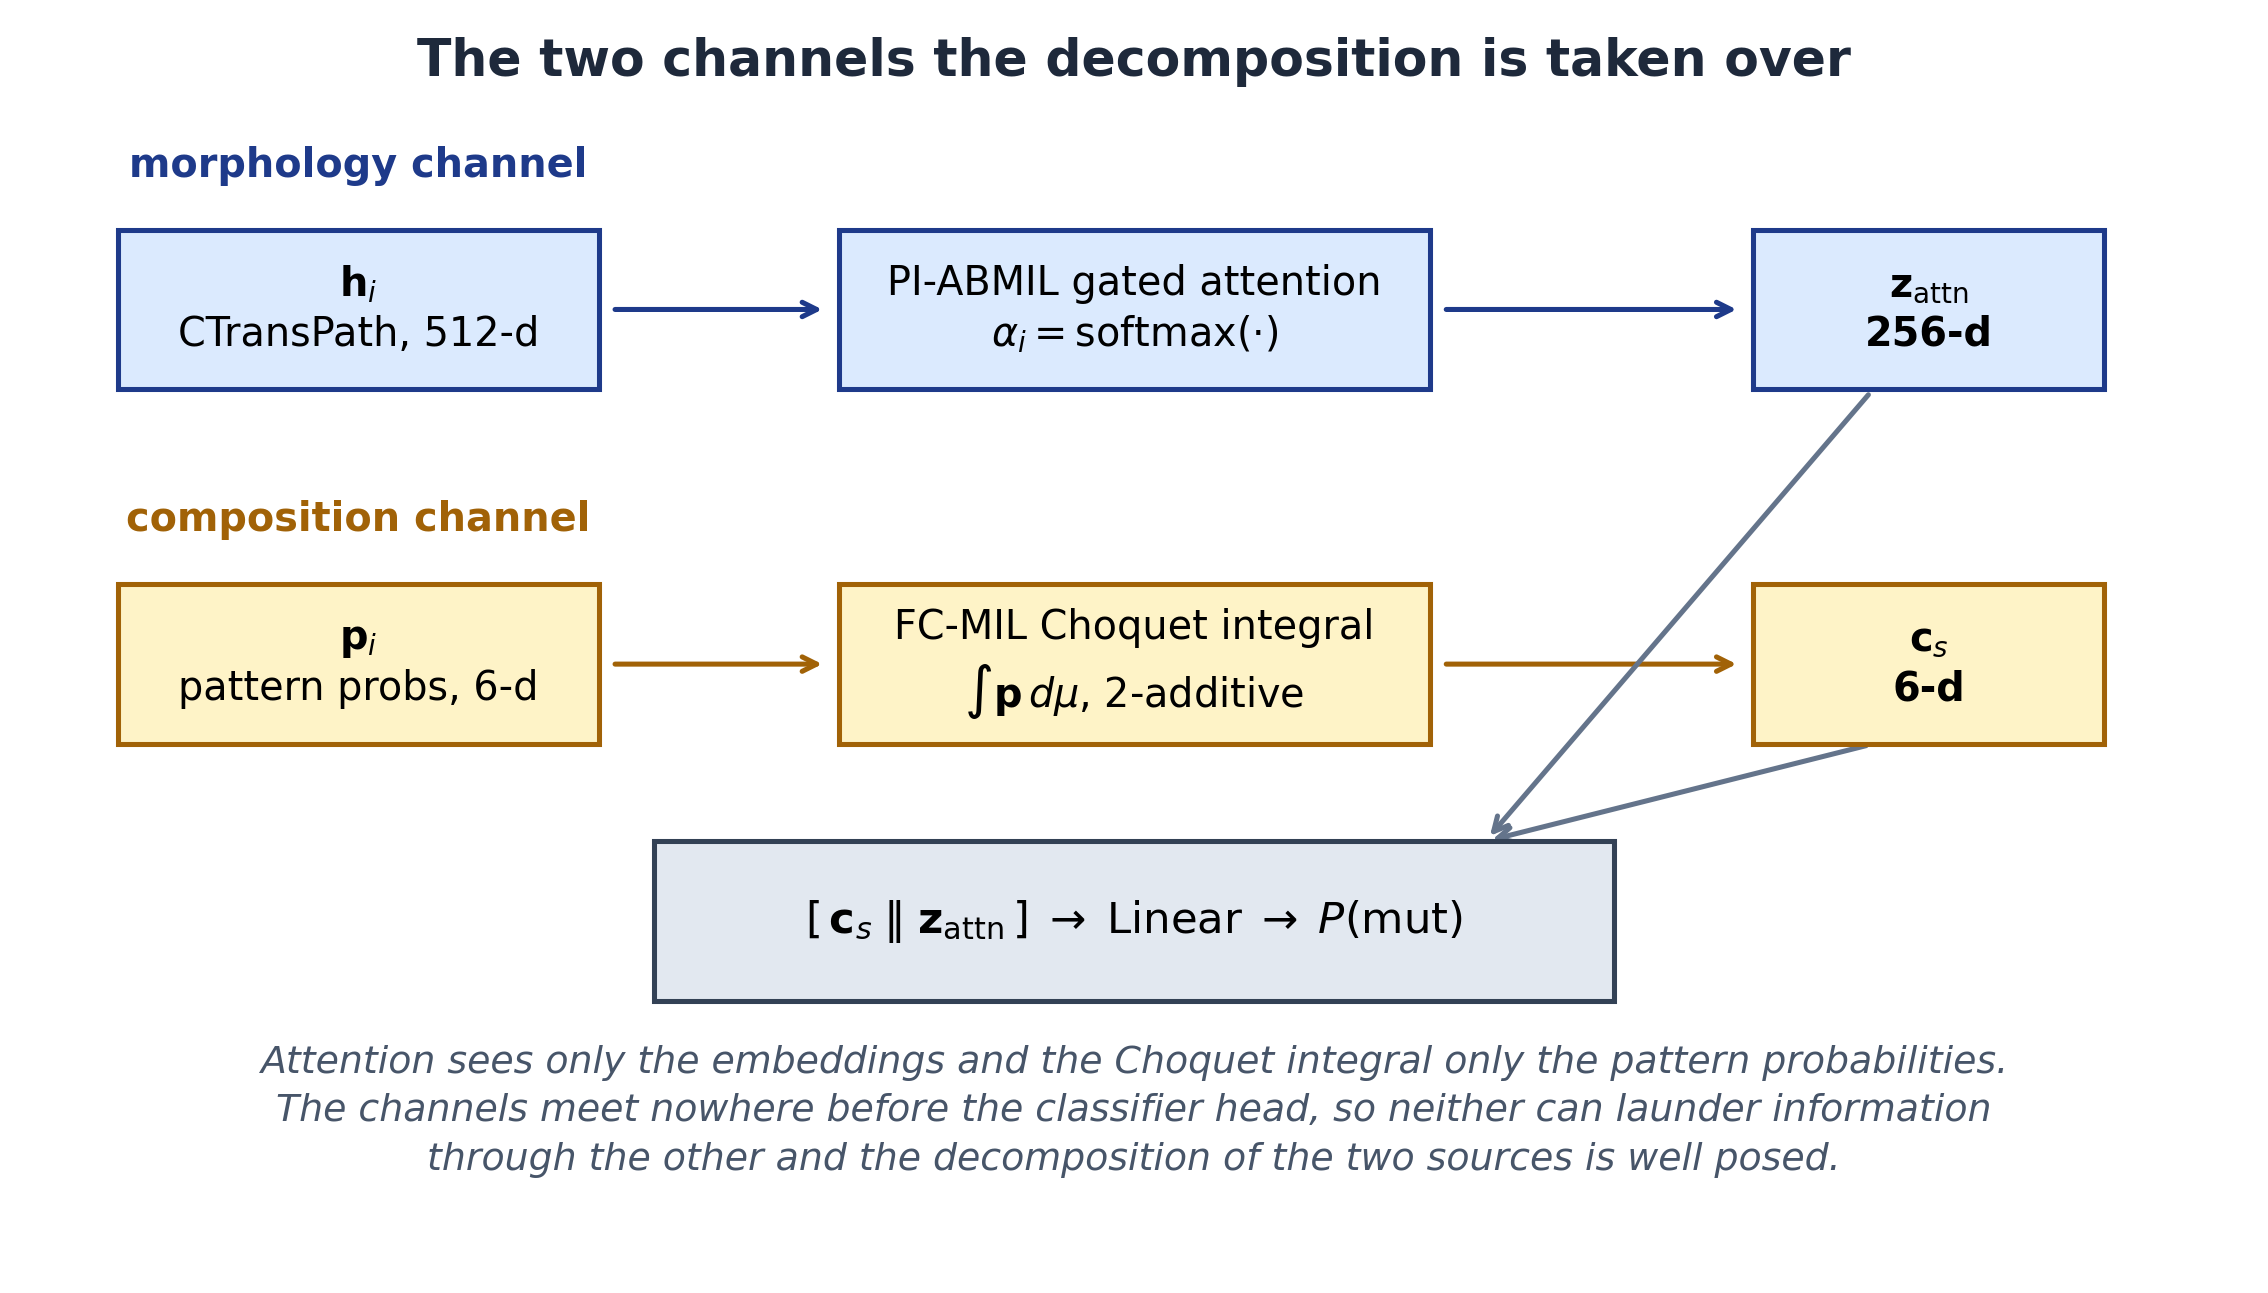
\includegraphics[width=\linewidth]{two_channel_architecture}
\caption{\textbf{The two-channel architecture in full.} Tile embeddings
from the frozen \ctranspath{} encoder and $6$-d fuzzy pattern
probabilities from the ANORAK-trained classifier remain disjoint until the
classifier head, which is what makes the decomposition of
\cref{eq:pid} well posed as a statement about two sources.}
\label{fig:two_channels}
\end{figure}

% --- Supplementary Fig. 7 ---
\begin{figure}[htbp]
\centering
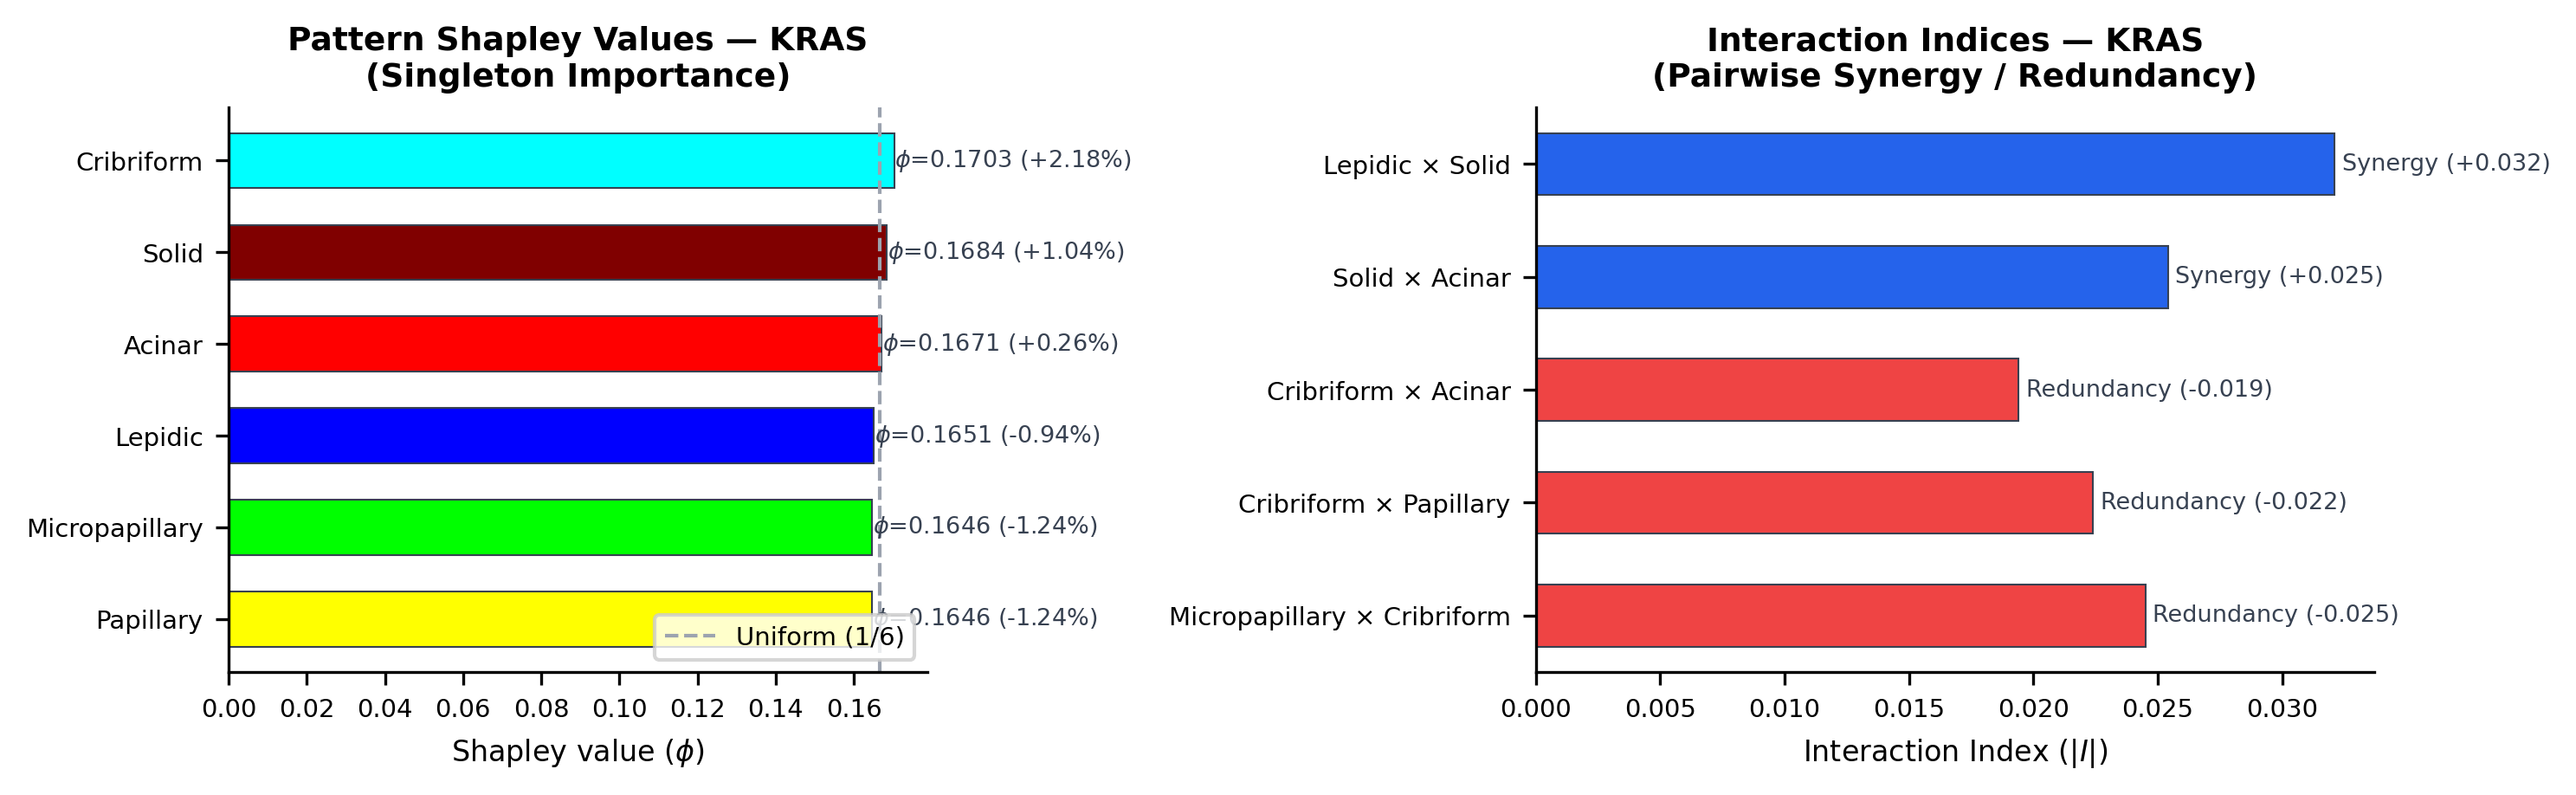
\includegraphics[width=\linewidth]{choquet_kras_55_7815}
\caption{\textbf{Full Choquet read-out for KRAS, rendered on slide
TCGA-55-7815.} The six singleton values $\phi_k$ and all
$15$ pairwise interaction indices $I_{jk}$ learned by the $2$-additive
fuzzy measure, from which the lepidic\,$\times$\,solid interaction of
$+0.032$ reported in the main text is read. These are parameters of the
fitted measure and are shared by every slide the model scores; the
figure is titled by slide because that is the interface the read-out is
served through, not because the values are estimated per slide. The
conditional test of whether this interaction buys accuracy where the
pair co-activates is \cref{tab:kras_coactivation}, and it is
unresolved.}
\label{fig:choquet_kras}
\end{figure}

% --- Supplementary Fig. 8 ---
\begin{figure}[htbp]
\centering
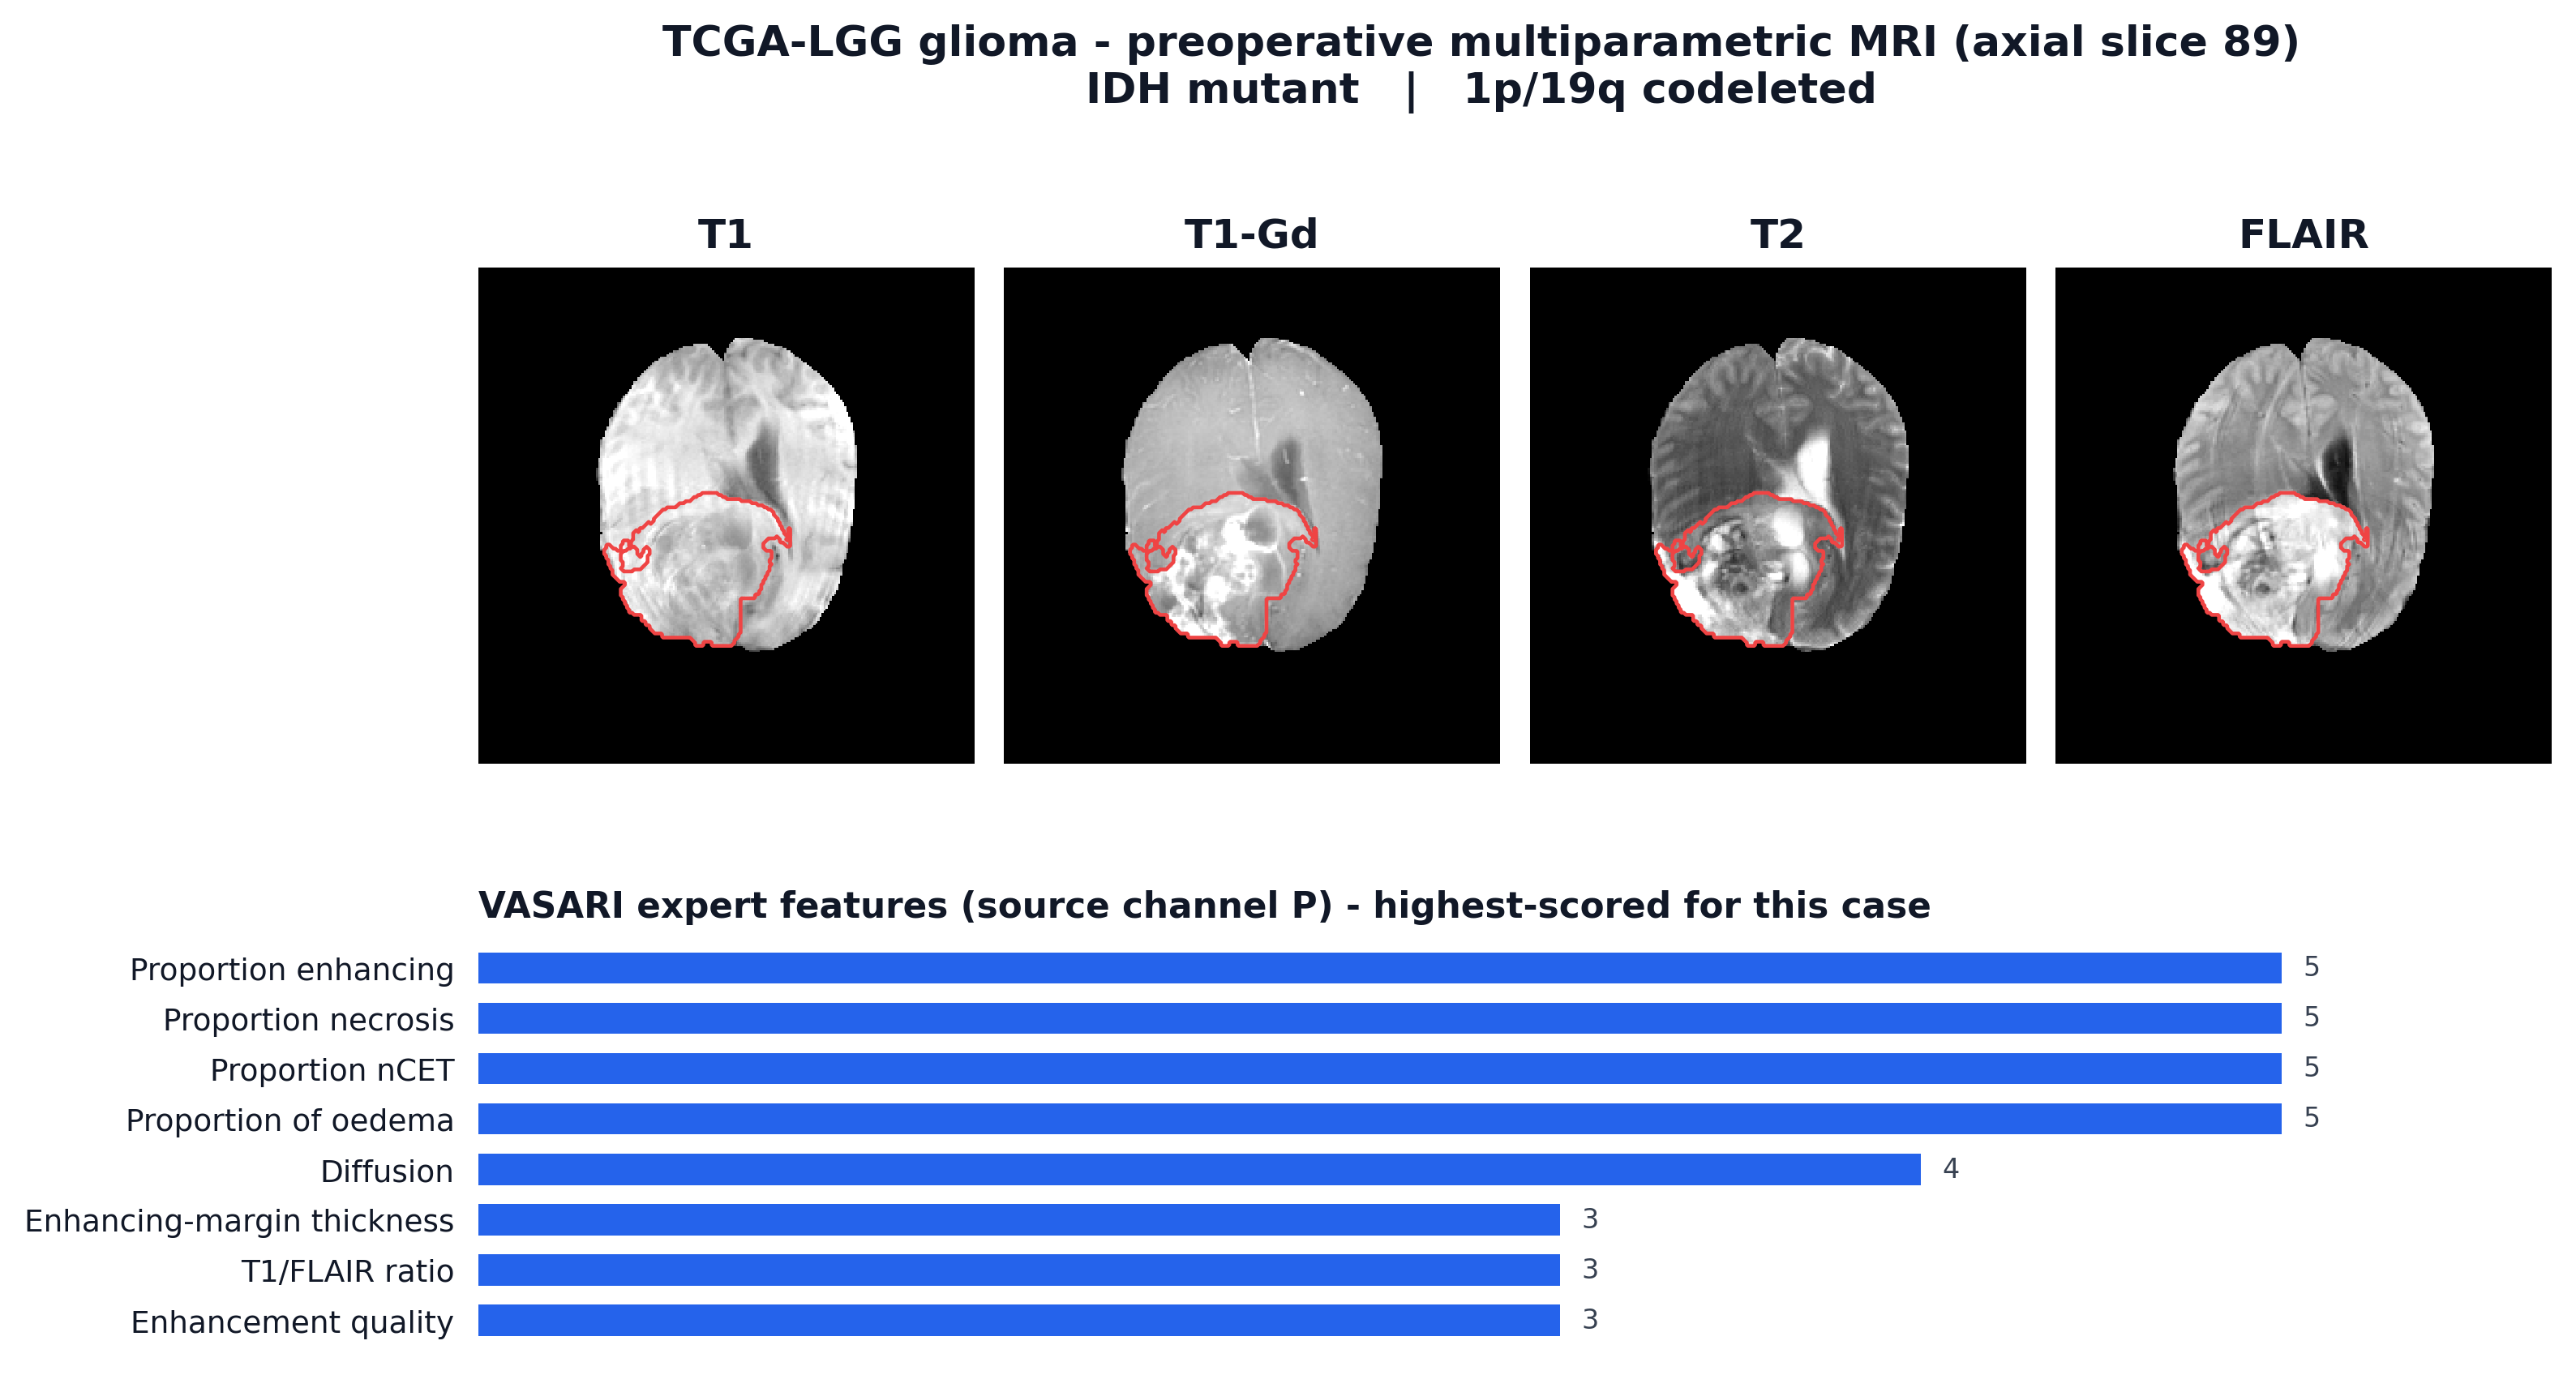
\includegraphics[width=\linewidth]{glioma_example}
\caption{\textbf{A real preoperative multiparametric MRI from a TCGA-LGG
glioma} (IDH-mutant, 1p/19q-codeleted)---the four co-registered sequences
(T1, T1-Gd, T2, FLAIR) the encoder $\mathbf{E}$ ingests, at the
tumour-centroid axial slice with the expert segmentation contour (red).
Below, the neuroradiologist VASARI scores for the same case, the source
channel $\mathbf{P}$: the radiological counterpart of the ANORAK growth
patterns in LUAD.}
\label{fig:glioma_example}
\end{figure}

% --- Supplementary Fig. 9 ---
\begin{figure}[htbp]
\centering
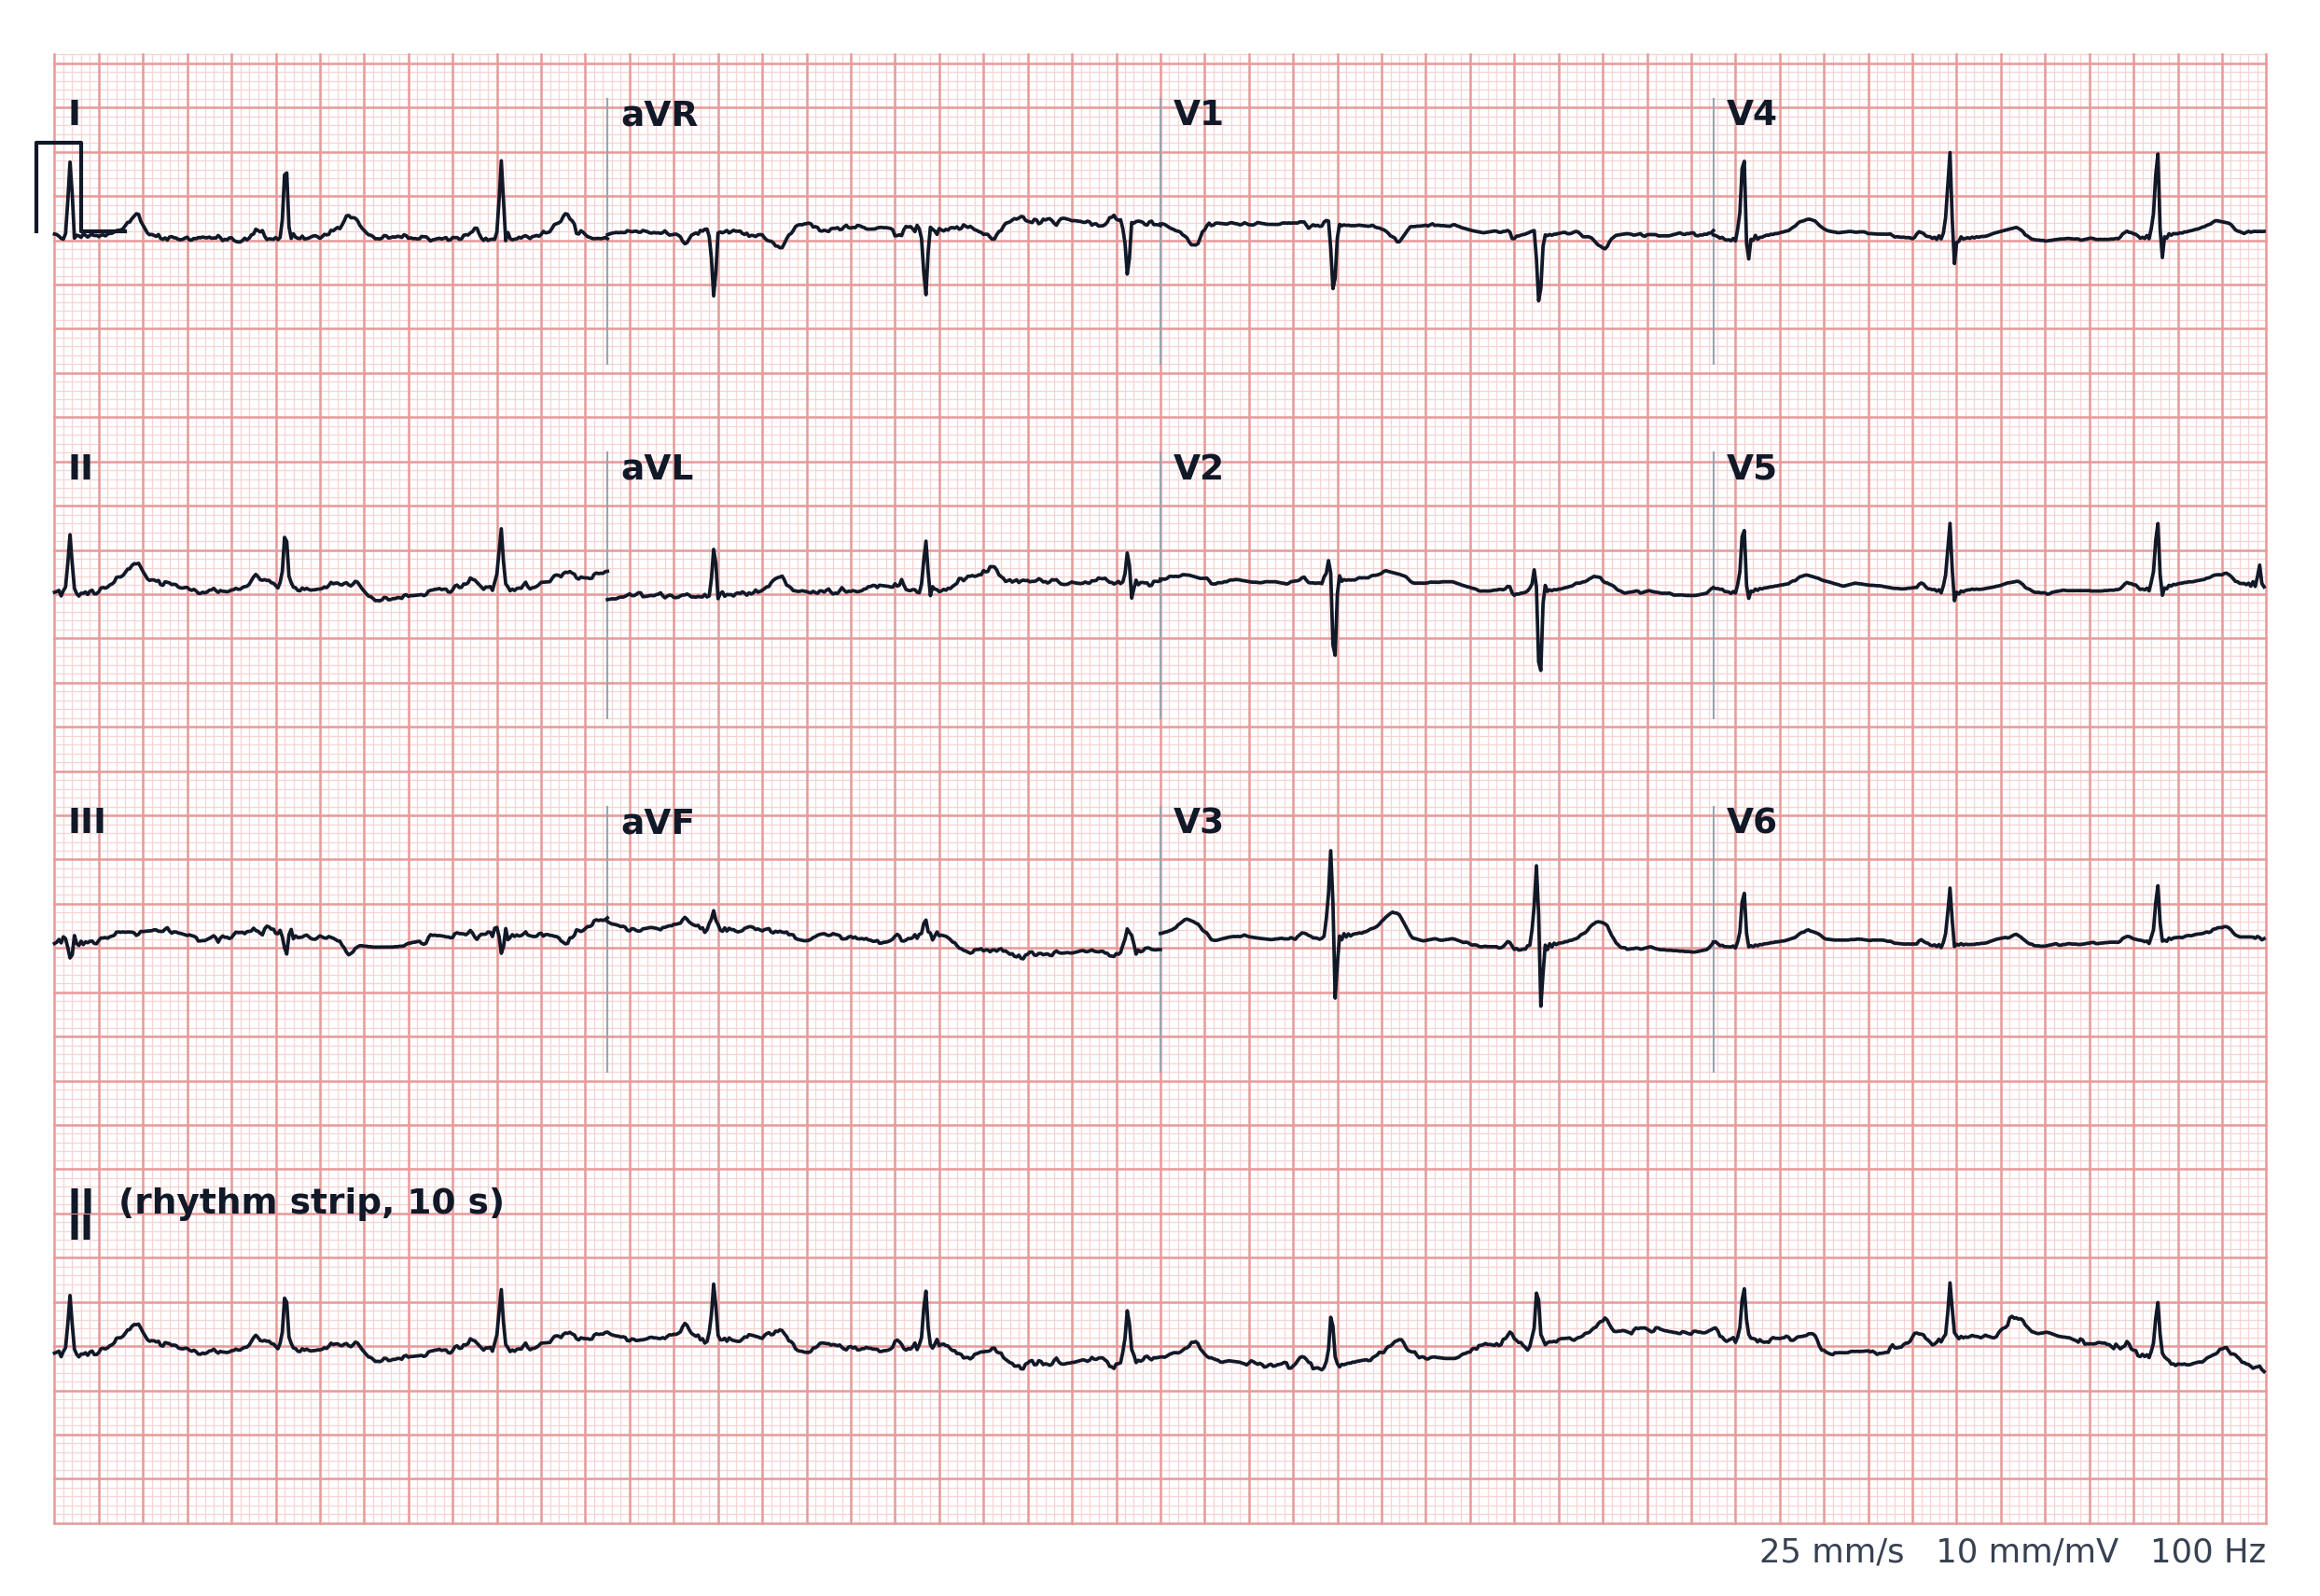
\includegraphics[width=\linewidth]{ecg_ptbxl_example}
\caption{\textbf{A real twelve-lead electrocardiogram from PTB-XL}
(a $37$-year-old woman, sinus rhythm, reported normal), in the standard
clinical $3\times4$ format with a lead-II rhythm strip
($25$\,mm/s, $10$\,mm/mV). This is the raw $100$\,Hz signal the encoder
ingests. Age and sex are recorded for every case but absent from the $71$
SCP-ECG statements forming the source channel, which is what makes the
recovery reported in \cref{tab:crossdomain_merged}
leakage-free.\cite{wagner2020ptbxl}}
\label{fig:ecg_ptbxl}
\end{figure}

% --- Supplementary Fig. 10 ---
\begin{figure}[htbp]
\centering
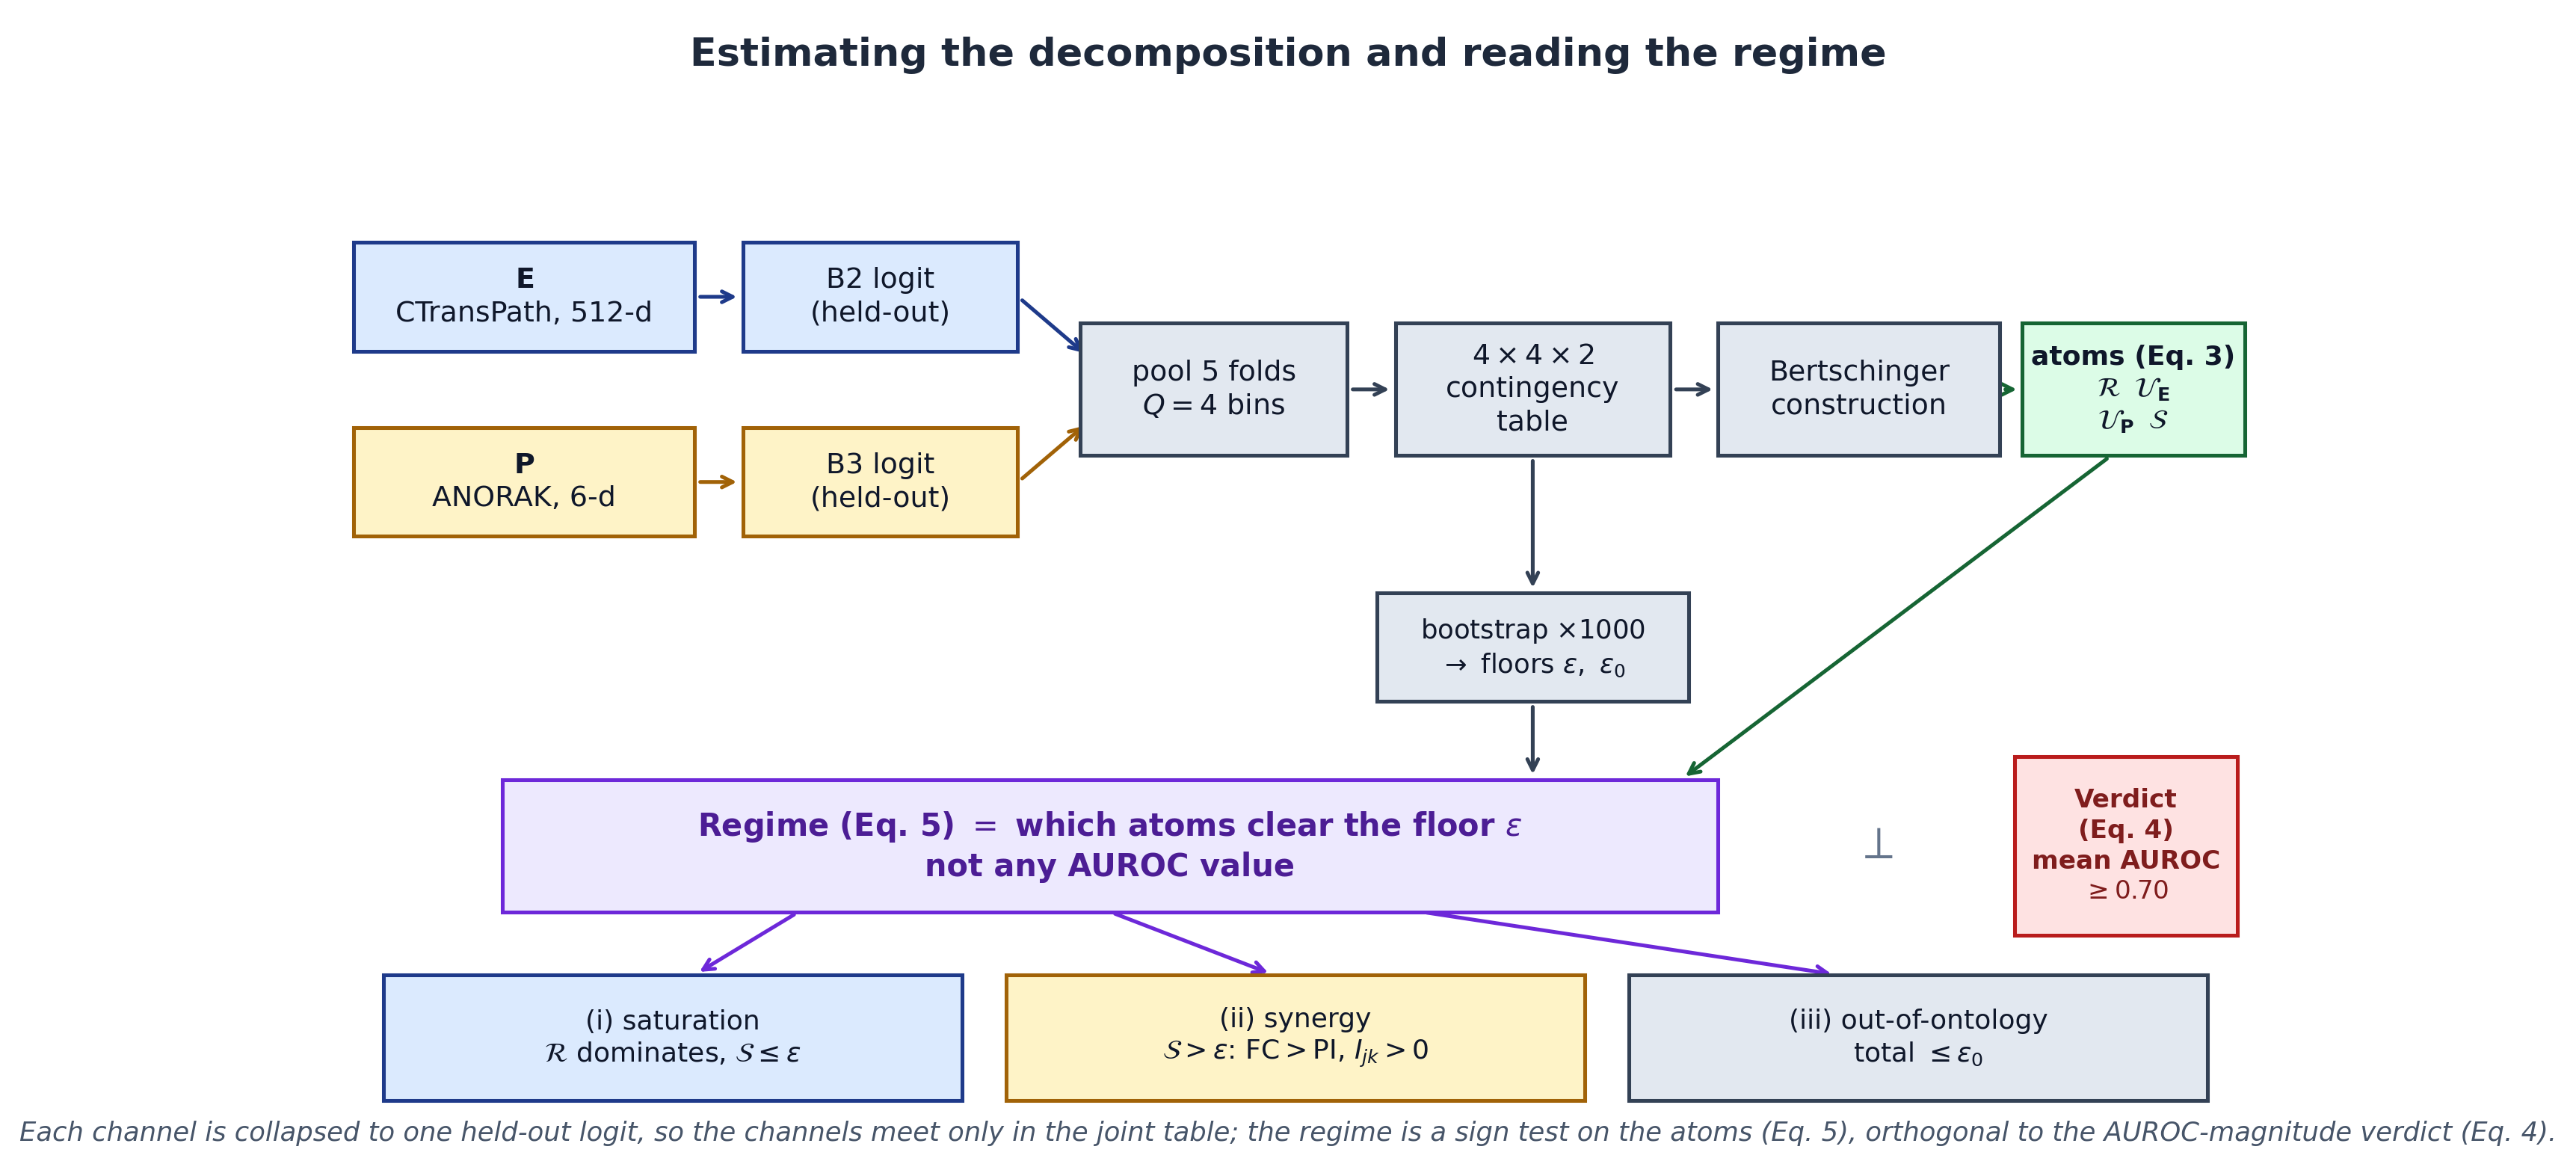
\includegraphics[width=\linewidth]{pid_estimator}
\caption{\textbf{Why the atoms are read as directional signatures rather
than estimated numerically.} The spread of the per-fold single-channel
\auroc{}s from which any plug-in atom estimate would be built, against
the size of the pattern-side effect such an estimate would have to
resolve.}
\label{fig:pid_estimator}
\end{figure}

\FloatBarrier
% ======================================================================
\section*{Supplementary Tables}
% ======================================================================

% --- Supplementary Table 1: levels of analysis ---
\begin{table}[htbp]
\centering
% Table tab:levels_of_analysis — the four levels at which this paper makes
% claims, and the scope of each. The point of the table is the last column:
% a verdict established at one level does not transfer to another, which is
% why the Conclusive/Inconclusive flag (population) and untranslatability
% (a statement about absent information at a stated level) are distinct.
\footnotesize
\setlength{\tabcolsep}{4pt}
\renewcommand{\arraystretch}{1.15}
\begin{tabularx}{\linewidth}{l c X X}
\toprule
\textbf{Level} & \textbf{Unit ($n$)} &
  \textbf{Quantities estimated here} &
  \textbf{Scope: what a claim at this level does, and does not, license} \\
\midrule
Population
  & gene $\times$ cohort (6)
  & Mean $\auroc$ over the five folds, \auprc{}, the \pid{} atoms of
    \cref{eq:pid} (read from model-side signatures, not estimated
    numerically), the regime assignment, and the
    Conclusive/Inconclusive verdict of \cref{eq:conclusive_verdict}
  & \emph{Licenses} statements about average discriminability over
    randomly drawn case pairs. \emph{Does not license} any statement
    about a named case: $\auroc$ is a ranking statistic and carries
    no posterior \\
\midrule
Patient
  & patient (444)
  & Mutation label; fold membership (stratification is at this level);
    $P(\mathrm{mut})$ pooled over that patient's slides
  & \emph{Licenses} the clinical decision---this is the unit a
    molecular test would be ordered for. \emph{Does not license}
    cohort claims, and inherits slide-level sampling of the tumour \\
\midrule
Slide
  & WSI (458)
  & $P(\mathrm{mut})$; $\mathbf{c}_s$, $\mathbf{z}_{\mathrm{attn}}$;
    the whole L1--L6 stack; Choquet--Shapley $\Phi_k$ and interaction
    indices $I_{jk}$; the fuzzy linguistic label
  & \emph{Licenses} the per-case argument with the pathologist and
    the localisation of evidence. \emph{Does not license}
    generalisation: one confident slide is not a cohort result \\
\midrule
Tile
  & $224\!\times\!224$ px ($\leq\!200$/slide)
  & $\tilde{\mathbf{x}}$, $\cos\theta_k$; pattern probabilities
    $\mathbf{p}_i$; attention $\alpha_i$; per-tile SHAP
  & \emph{Licenses} where in the tissue the evidence sits.
    \emph{Does not license} a slide-level call on its own: attention
    mass is not probability \\
\bottomrule
\end{tabularx}
\begin{flushleft}\footnotesize
The three-regime taxonomy and the Conclusive/Inconclusive verdict are
defined at the population level only.
The consequence that matters clinically is that an Inconclusive
verdict is compatible with four distinct states of the world, which
the cohort mean cannot separate: information absent at every level
(strict untranslatability, the KEAP1 candidate); information present
in a morphologically defined \emph{subpopulation} and therefore
diluted in the cohort average (KRAS, where the cohort mean is $0.517$
yet TCGA-55-7815 carries $P=0.965$ with a coherent
lepidic$\times$solid Choquet readout); information present but
unestimable at the available positive-set size (RBM10, $n_+=32$); and a
\emph{heterogeneous target}, in which the gene-level label unions
variants with different morphological correlates whose signals partly
cancel in the mixture. The last is the same dilution mechanism as the
second, relocated from the cases to the label definition, and it is
untested here: splitting \textit{EGFR} by variant
(exon-19 deletion, L858R, exon-20 insertion) leaves every subset far
below the estimation floor, so we flag it as a confound on regime~(iii)
rather than resolving it.
Only the first is untranslatability.
\end{flushleft}

\caption{\textbf{The four levels of analysis, the quantities estimated at
each, and the scope of the claims each supports.} The
Conclusive/Inconclusive verdict and the three-regime taxonomy are
population-level objects; the per-slide read-outs (L1--L6, Methods) are
slide-level and tile-level objects; neither transfers to the other. KRAS is the
canonical illustration, and in both directions: a confident per-slide
call does not lift the population verdict, and a population-level
interaction weight does not descend into per-case evidence
(\cref{tab:kras_coactivation}). Only the name of the unit and whether it is a bag
or a single instance change when the framework moves to glioma MRI or to
the electrocardiogram, which is the precise sense in which the framework,
and not the model weights, transfers.}
\label{tab:levels_of_analysis}
\end{table}

% --- Supplementary Table 2: literature comparison ---
\begin{table}[htbp]
\centering
% Table tab:literature_comparison_resultssec — comparison of mutation prediction
% methods in NSCLC. Synced with thesis Table 2.5 (ch02_background.tex, lines
% 1299-1331): seven prior studies + this work's two MIL conditions.
% AUROC values are means or ranges across the cited paper's CV protocol;
% daggers (^\dagger) indicate values approximated from published figures.
% Wide table: wrapped in \resizebox so it scales to the printed column width.
\resizebox{\linewidth}{!}{%
\setlength{\tabcolsep}{4pt}
\begin{tabular}{l c l r l c c c c c c}
\toprule
\textbf{Study} & \textbf{Year} & \textbf{Journal} & $\boldsymbol{N}$ &
  \textbf{Method} &
  \textit{TP53} & \textit{EGFR} & \textit{KRAS} &
  \textit{STK11} & \textit{KEAP1} & \textit{RBM10} \\
\midrule
Coudray~et~al.\cite{coudray2018classification} &
  2018 & Nat.\ Med.\ & 382 & Inception-v3 e2e\textsuperscript{*} &
  0.760 & 0.826 & 0.733 & 0.856 & 0.675 & --- \\
Kather~et~al.\cite{kather2020pancancer} &
  2020 & Nat.\ Cancer & 17{,}355 & ShuffleNet+att.\ &
  0.65--0.72$^{\dagger}$ & 0.63--0.68$^{\dagger}$ & 0.60--0.65$^{\dagger}$ & --- & --- & --- \\
Saldanha~et~al.\cite{saldanha2023npj} &
  2023 & npj Prec.\ Onc.\ & 676 & RetCCL+attMIL &
  --- & 0.76\textsuperscript{\P} & --- &
  --- & --- & --- \\
Zhao~et~al.\cite{zhao2025deepgem} (DeepGEM) &
  2025 & Lancet Onc.\ & 3{,}637 & co-supervised MIL &
  0.82--0.96\textsuperscript{$\ddagger$} & 0.945\textsuperscript{$\ddagger$} & 0.82--0.96\textsuperscript{$\ddagger$} & --- & --- & --- \\
Campanella~et~al.\cite{campanella2025eagle} (EAGLE) &
  2025 & Nat.\ Med.\ & 8{,}461 & FM fine-tuning &
  --- & 0.890 & --- & --- & --- & --- \\
Wang~et~al.\cite{wang2024chief} (CHIEF) &
  2024 & Nature & 60{,}530 & FM, pan-cancer &
  ---\textsuperscript{\S} & $>$\,0.70 & --- & --- & --- & --- \\
\midrule
\multirow{3}{*}{\textbf{This work}} & \multirow{3}{*}{2026} & \multirow{3}{*}{---} & \multirow{3}{*}{\textbf{458}}
  & B2 (encoder only)\textsuperscript{\textbardbl} & \textbf{0.661} & \textbf{0.582} & \textbf{0.517} & 0.591 & \textbf{0.488} & 0.536 \\
  & & & & \piabmil{} & 0.658 & 0.580 & 0.516 & 0.578 & 0.446 & \textbf{0.552} \\
  & & & & \fcmil{} & 0.646 & 0.567 & 0.506 & \textbf{0.608} & 0.460 & 0.528 \\
\bottomrule
\end{tabular}%
}
\begin{flushleft}\footnotesize
\textsuperscript{*}The whole Coudray row is the per-slide AUC obtained by
averaging the predicted tile probabilities (their Fig.~3 table), measured on a
$62$-slide held-out test set. The widely quoted $0.733$--$0.856$ is the range
over the six genes they call predictable, and its endpoints are \textit{KRAS}
and \textit{STK11}, not a per-gene value for either \textit{TP53} or any other
gene. Their intervals are correspondingly wide, e.g.\ \textit{STK11}
$[0.709,0.964]$ and \textit{KEAP1} $[0.466,0.865]$.
$^{\dagger}$Kather~et~al.\ report LUAD per-gene AUROCs only in a bar chart
(their Extended Data Fig.~2); the values shown are read from that figure and lie
within the paper's stated LUAD range of $0.60$--$0.78$ (3-fold CV on TCGA).
\textsuperscript{\P}Saldanha~et~al.\ report only \textit{EGFR} for LUAD
(AUROC $0.76\!\pm\!0.03$, external validation on CPTAC); the other LUAD
target genes are not individually reported in the source.
\textsuperscript{$\ddagger$}DeepGEM reports an overall cross-gene AUC range
on the public TCGA set (0.82--0.96) rather than per-gene values; EGFR is
the strongest (${\approx}0.945$) and STK11 is not among its target genes.
\textsuperscript{\S}CHIEF's validated LUAD-specific result is EGFR
($>0.70$ in held-out and independent sets); its strong TP53 signal is in
other tumour types (low-grade glioma, adrenal, endometrial), not LUAD.
EAGLE's 0.890 is the prospective silent-trial AUC (retrospective means:
internal 0.847, external 0.870).
Cohort sizes ($N$) are slide counts.
``---'' indicates the gene was not reported in the corresponding study;
Coudray is the only prior study reporting \textit{STK11} and \textit{KEAP1}
individually, and \textit{RBM10} is reported by none of them.
\textsuperscript{\textbardbl}Our rows are pooled out-of-fold \auroc{},
patient-preserved folds, averaged over five seeds
(\cref{tab:mutation_luad_resultssec}); B2 is the encoder-only ceiling
baseline and is included because it, not either fusion condition, is the
best this cohort yields on four of six genes.
\par\smallskip
\textbf{This row is not commensurable with the rows above it, and the gap
should not be read as a method comparison.} Ours are scored under nested
cross-validation, with early stopping on an inner split and the outer fold
scored exactly once, on a cohort restricted to adenocarcinoma cases with a
mutation call and cleared of solid-tissue-normal sections. The prior line
predominantly reports values selected on the same fold they are scored on,
and on inventories that retain squamous and normal sections. Removing those
two sources of optimism is what separates the two blocks; a like-for-like
comparison would require rerunning each prior method under this protocol,
which we do not do. The audit of what these cohorts can resolve at all is
\cref{tab:literature_power_audit}.
\end{flushleft}

\caption{\textbf{Per-gene \auroc{} against the published
mutation-prediction competition on LUAD.} This work reports six driver
genes simultaneously on the public TCGA-LUAD cohort under a single MIL
aggregator; prior work typically reports two to three genes on either the
same public cohort or on proprietary cohorts an order of magnitude larger.
Within \textbf{This work}, bold marks the better of the two aggregators
per gene. No value is bolded \emph{across} studies: the protocols are not
comparable, mixing held-out test sets with cross-validation and public
with proprietary cohorts, so a column maximum would not identify a better
method. A per-gene \auroc{} also does not answer the question this paper
asks---whichever study reports the higher one, the number does not say
whether the signal lies inside the source ontology or outside it, and
that is what decides whether the next experiment is a larger cohort, a
richer vocabulary or a different modality. No study below reports a regime
or a per-target verdict. The comparison is developed in Supplementary
Note~2.}
\label{tab:literature_comparison}
\end{table}

% --- Supplementary Table 3: CPTAC frozen transfer ---
\begin{table}[htbp]
\centering
% Table tab:cptac_transfer — empirical within-domain cohort-transfer result.
% CPTAC-LUAD (498 slides, 106 genotyped patients with matched H&E), the frozen
% TCGA-trained pipeline applied off-the-shelf (no stain normalisation, colour
% calibration or domain adaptation). "CPTAC AUROC" is the patient-level read-out
% (slides mean-pooled, the pre-registered aggregation) with a 2000-sample
% bootstrap 95% CI; the slide-level column assigns each of the 498 slides its
% patient's genotype. TCGA AUROC is the best-aggregator value reported
% for the LUAD cohort in this paper. The "Reinhard" column re-runs the same
% patient-level read-out after Reinhard stain normalisation of every tile to a
% representative TCGA-LUAD reference; it isolates a global colour/stain cast
% as a cause.
\footnotesize
\setlength{\tabcolsep}{4pt}
\renewcommand{\arraystretch}{1.2}
\begin{tabular}{l c c c c c c}
\toprule
\textbf{Gene} & \textbf{Regime (TCGA)} & \textbf{TCGA} & \textbf{$n_+$} &
  \textbf{CPTAC AUROC} & \textbf{Reinhard} & \textbf{slide} \\
              &                        & \textbf{AUROC} & \textbf{(/$106$)} &
  \textbf{($95\%$ CI)} & \textbf{AUROC} & \textbf{AUROC} \\
\midrule
\textit{TP53}$^\dagger$  & (i) directional  & $0.661$ & $55$ & $0.53$ ($0.42$--$0.64$) & $0.48$ & $0.49$ \\
\textit{EGFR}            & (i) directional  & $0.582$ & $36$ & $0.57$ ($0.45$--$0.70$) & $0.57$ & $0.55$ \\
\textit{KRAS}            & (ii-b) not supp. & $0.517$ & $32$ & $0.59$ ($0.48$--$0.71$) & $0.59$ & $0.57$ \\
\textit{STK11}           & (iii) directional& $0.608$ & $20$ & $0.46$ ($0.34$--$0.59$) & $0.48$ & $0.43$ \\
\textit{KEAP1}           & encoder-ceiling null & $0.488$ & $12$ & $0.43$ ($0.23$--$0.64$) & $0.41$ & $0.50$ \\
\textit{RBM10}           & est.\ floor      & $0.552$ & $5$  & $0.40$ ($0.23$--$0.55$) & $0.51$ & $0.43$ \\
\bottomrule
\end{tabular}
\begin{flushleft}\footnotesize
$^\dagger$\textit{TP53} ($n_+\!=\!55$) and \textit{EGFR} ($n_+\!=\!36$)
clear the $n_+\!=\!32$ estimation floor in the
genotyped-with-imaging subset ($n\!=\!106$), and \textit{KRAS} sits
exactly at it; the remaining rows are underpowered
and their near-chance values are, as pre-registered, statements about power.
CPTAC AUROC is the patient-level read-out (slides mean-pooled, the
pre-registered aggregation) with a $2000$-sample bootstrap $95\%$ CI; the
slide-level column ($n\!=\!498$, each slide inheriting its patient's genotype)
and the max, top-$2$, top-$3$ and largest-slide aggregators (not shown) place
every gene within $\pm0.06$ of the tabulated value, so the collapse is not an
artefact of patient-level pooling. No off-the-shelf CPTAC AUROC exceeds $0.62$.
Only \textit{TP53} is both well powered and high enough in TCGA for the
transfer to be informative, and there its interval excludes the TCGA point
($0.661$ lies above the upper limit $0.64$). Both cohorts return
Inconclusive---no LUAD target clears $0.70$ in either---so what the transfer
adds is not a change of verdict but the sharper statement that the
\emph{value} does not survive the move.
The remaining rows cannot carry that argument. \textit{EGFR} starts at
$0.582$ and lands at $0.57$, a move too small to interpret in a cohort this
size; \textit{KRAS} starts at $0.517$ and rises to $0.59$, in the opposite
direction; and \textit{STK11}, \textit{KEAP1} and \textit{RBM10} are
underpowered here. The transfer conclusion therefore rests on \textit{TP53}
alone, and only for \textit{TP53} was there a value worth losing. The \textbf{Reinhard} column
repeats the patient-level read-out after Reinhard stain normalisation of every
tile to a representative TCGA-LUAD reference
(\texttt{--stain-method reinhard}): it does not recover transfer
(\textit{TP53} $0.48$ at the patient level, at most $0.54$ across the other
five read-outs, its $95\%$ CI still excluding the TCGA point; no aggregator
recovers the TCGA value for any gene), so the collapse is not a global
colour/stain cast either. Macenko stain-matrix normalisation was
not tested and is left to future work.
Every value in this table is a \emph{frozen-pipeline} read-out, and measures
whether the learned decision function survives the move between cohorts. It
is not a measure of whether CPTAC slides carry the signal: re-fitting the four
aggregation conditions inside CPTAC, with only the representation carried
over, reaches \textit{TP53} $0.698$ against the TCGA $0.661$
(\cref{tab:cptac_refit})---slightly \emph{above} the source cohort---so the
collapse tabulated here is a property of the transported model rather than of
the encoder or of the tissue.
\end{flushleft}

\caption{\textbf{Cohort transfer to CPTAC-LUAD: the frozen TCGA-trained
pipeline applied off-the-shelf} ($498$ slides, $106$ genotyped patients).
Read this way the TCGA verdicts do not transfer. What fails, however, is
the transported decision function and not the tissue, so no assignment is
licensed as near-intrinsic on this evidence, but neither is the coupling
itself cohort-local. Per-gene values, the aggregator and
stain-normalisation controls and the power caveat are set out below the
table.}
\label{tab:cptac_transfer}
\end{table}

% --- Supplementary Table 4: CPTAC refit ---
\begin{table}[htbp]
\centering
% Table tab:cptac_refit — CPTAC-internal refit of the four conditions.
% Only the representation is frozen (CTransPath embeddings + ANORAK pattern
% probabilities recomputed on CPTAC tiles); the four aggregation conditions are
% re-fitted with 5-fold patient-disjoint CV inside CPTAC. TP53 only: it is the
% one gene clearing the n_+=32 estimation floor in this subset (n_+=55).
% "Native" tiles CPTAC at level 0 exactly as the TCGA pipeline does. "FOV-matched"
% centre-crops and rescales every tile so its physical field of view matches a
% 40x TCGA tile (target 0.25 micron/pixel), testing the scanner-magnification
% account of the transfer failure.
\footnotesize
\setlength{\tabcolsep}{6pt}
\renewcommand{\arraystretch}{1.2}
\begin{tabular}{l c c}
\toprule
\textbf{Condition (\textit{TP53}, $n_+\!=\!55$)} & \textbf{Native} & \textbf{FOV-matched} \\
\midrule
B2 \quad encoder only                & $0.665$ & $0.561$ \\
B3 \quad pattern channel only        & $0.667$ & $0.570$ \\
\piabmil{} \quad concat fusion       & $0.698$ & $0.632$ \\
\fcmil{} \quad $2$-additive Choquet  & $0.669$ & $0.538$ \\
\midrule
$\piabmil{}-\mathrm{B2}$             & $+0.032$ & $+0.073$ \\
Regime, point estimate               & (ii-a) & (ii-a) \\
Regime, adjudicated                  & unresolved & unresolved \\
$P(\text{regime reproduces TCGA})$   & $0.214$ & $0.129$ \\
\midrule
\multicolumn{3}{l}{\emph{Reference:} TCGA-LUAD $0.661$; frozen transfer $0.53$
($0.42$--$0.64$), \cref{tab:cptac_transfer}} \\
\bottomrule
\end{tabular}
\begin{flushleft}\footnotesize
Pooled out-of-fold AUROC over $5$ patient-disjoint folds on the $106$
genotyped CPTAC patients ($498$ slides). Only the \emph{representation} is
carried over from TCGA; the aggregation conditions are re-fitted inside CPTAC,
which is the comparison the frozen-pipeline test of \cref{tab:cptac_transfer}
cannot make. The native arm reaches $0.698$ against the TCGA value of $0.661$,
and its encoder-only baseline ($0.665$) lands within $0.004$ of the TCGA
encoder-only baseline ($0.661$). The morphology-to-genotype coupling for
\textit{TP53} is therefore present in CPTAC at fully comparable strength---if
anything marginally stronger---and the off-the-shelf collapse to $0.53$ is a
property of the transported decision function, not of the encoder or of the
tissue.
The \textbf{FOV-matched} arm is a negative control for the
scanner-magnification account (TCGA-LUAD is $76.4\%$ $40\times$, CPTAC-LUAD
$98.6\%$ $20\times$): matching the physical field of view lowers every
condition and inflates fold-to-fold spread (B2 ranges $0.373$--$0.918$ across
folds, against $0.587$--$0.791$ natively), so scale mismatch is not the
mechanism, though the centre-crop is itself lossy and the arm is not evidence
in the opposite direction either.
Regime adjudication follows the noise-aware rule of the Methods: the deciding
contrast is $\piabmil{}-\mathrm{B2}$, whose $2000$-sample paired-bootstrap
$95\%$ CI is $-0.041$ to $+0.102$ natively and $-0.038$ to $+0.174$
FOV-matched. Both span zero, so the point-estimate read of (ii-a) is
\emph{not} separable from noise and no regime is asserted; the cohort neither
confirms nor contradicts the TCGA reading of~(i).
\end{flushleft}

\caption{\textbf{Re-fitting the four conditions inside CPTAC-LUAD, with
only the representation carried over from TCGA.} This is the comparison
the frozen-pipeline transfer of \cref{tab:cptac_transfer} cannot make, and it
separates the two readings that transfer alone leaves open. The recovered
values, the field-of-view control and the regime adjudication under the
noise-aware rule are set out below the table.}
\label{tab:cptac_refit}
\end{table}

% --- Supplementary Table 5 ---
\begin{table}[htbp]
\centering
% Table tab:atom_operationalization — how each atom of Eq. (eq:pid) is read
% from the model, not estimated numerically. Maps the four PID atoms to the
% model-side signature, the directional decision rule, the interpretability
% level(s) that expose it, and the regime it drives. All rules are on the
% four training conditions B2/B3/PI/FC and the sign of the Choquet index.
\footnotesize
\setlength{\tabcolsep}{4pt}
\renewcommand{\arraystretch}{1.25}
\begin{tabularx}{\linewidth}{@{}c X X c c@{}}
\toprule
\textbf{Atom} & \textbf{Model-side signature (how it is read)} &
  \textbf{Decision rule (directional)} & \textbf{Level} & \textbf{Regime} \\
\midrule
$\Ired$
  & Fusion is a no-op on top of the encoder; SHAP places the slide-level
    contribution on the embedding
  & $\mathrm{PI}\!\approx\!\mathrm{FC}\!\approx\!\mathrm{B2}$ and
    $I_{jk}\!\le\!0$
  & L3 & (i) \\
$\Iuni{\mathbf{E}}$
  & Encoder-only far exceeds vocabulary-only; zeroing the embedding costs
    most of the \auroc{}, zeroing the pattern channel almost none
  & $\mathrm{B2}\!\gg\!\mathrm{B3}$; asymmetric L5 ablation
  & L3, L5 & (iii) \\
$\Iuni{\mathbf{P}}$
  & Additive concat fusion recovers signal neither channel carries alone
    (complementary unique information)
  & $\mathrm{PI}\!>\!\max(\mathrm{B2},\mathrm{B3})$,
    $\mathrm{FC}\!\approx\!\mathrm{PI}$
  & conditions, L5 & (ii-a) \\
$\Isyn$
  & Only the non-additive aggregator recovers the signal; a supra-additive
    fuzzy measure on a pattern pair
  & $\mathrm{FC}\!>\!\mathrm{PI}$ and $\max_{j<k} I_{jk}\!>\!0$
    \emph{and} the FC${-}$PI contrast larger in the high than in the low
    co-activation stratum of that pair, under both protocols
  & L4 & (ii-b) \\
\bottomrule
\end{tabularx}
\begin{flushleft}\footnotesize
The four atoms of \cref{eq:pid} and the observable by which each is read.
$\mathrm{B2}$/$\mathrm{B3}$/$\mathrm{PI}$/$\mathrm{FC}$ are the four training
conditions (encoder only, vocabulary only, concat fusion, 2-additive
Choquet); $I_{jk}$ is the learned Choquet pair-interaction index (L4).
These are \emph{directional} signatures, not numerical estimates of the
atoms; atom names follow the Bertschinger
convention.\cite{bertschinger2014unique} The ``unestimable'' sub-state of regime~(iii)
(e.g.\ \textit{RBM10}) arises when the total $I(\mathbf{P},\mathbf{E};Y)$
itself sits near the estimation floor, so a non-empty pattern-side atom
cannot be resolved from noise at the available positive-set size.
\end{flushleft}

\caption{\textbf{How each atom of \cref{eq:pid} is read from the model.}
Every atom is mapped to the model-side signature that evidences it, the
directional decision rule on the four training conditions, the
interpretability level(s) that expose it, and the regime it drives. The
signatures are read, not numerically estimated; atom names follow the
Bertschinger convention.\cite{bertschinger2014unique}}
\label{tab:atom_operationalization}
\end{table}

% --- Supplementary Table 6 ---
\begin{table}[htbp]
\centering
% Table tab:kras_coactivation — the conditional test of regime (ii-b) on KRAS.
% Strata are terciles of patient-level lepidic x solid co-activation, computed
% from the ANORAK pattern head alone and therefore independent of every
% mutation-side quantity in the table. FC-PI intervals are the hierarchical
% bootstrap of Methods (2000 resamples, seeds resampled before patients,
% site-clustered under the site-preserved protocol).
% Source: stratified_luad_contrast.py, stratified_summary.json, from the run
% stratified_kras_final (seeds 42, 142, 242, 342, 442), which is the same
% five-seed basis as tab_mutation_luad. An earlier draft of this table carried
% the three-seed stage-1 values (high-low -0.029 and -0.011); those are
% superseded. The two differ materially in one place: under site preservation
% the point estimate moves from -0.011 to +0.025, so the high-low estimates
% now disagree in sign across protocols rather than agreeing on negative.
\footnotesize
\setlength{\tabcolsep}{5pt}
\renewcommand{\arraystretch}{1.15}
\begin{tabular}{l c c c c c}
\toprule
\textbf{Co-activation} & \textbf{Patients} & \textbf{KRAS$^{+}$} &
  \textbf{Prevalence} & \multicolumn{2}{c}{\textbf{FC${-}$PI $\Delta\auroc$ [95\% CI]}} \\
\cmidrule(lr){5-6}
\textbf{stratum} & & & & \textbf{Patient-preserved} & \textbf{Site-preserved} \\
\midrule
Low    & $148$ & $33$ & $22.3\%$
  & $-0.004$ $[-0.072,\,{+}0.062]$ & $-0.028$ $[-0.102,\,{+}0.042]$ \\
Mid    & $148$ & $42$ & $28.4\%$
  & $-0.000$ $[-0.078,\,{+}0.086]$ & ${+}0.021$ $[-0.044,\,{+}0.095]$ \\
High   & $148$ & $49$ & $33.1\%$
  & $-0.028$ $[-0.095,\,{+}0.041]$ & $-0.003$ $[-0.095,\,{+}0.079]$ \\
\midrule
\textbf{High ${-}$ Low} & --- & --- & ---
  & $\mathbf{-0.024}$ $[-0.117,\,{+}0.072]$
  & $\mathbf{+0.025}$ $[-0.090,\,{+}0.141]$ \\
\bottomrule
\end{tabular}
\begin{flushleft}\footnotesize
Terciles of patient-level lepidic$\,\times\,$solid co-activation, defined as
$\min(f_{\text{lep}}, f_{\text{sol}})$ over the slide's hard pattern
assignment and averaged across a patient's slides
($n\!=\!444$ patients, $458$ slides). The cut uses only the ANORAK pattern
head, so it is independent of every mutation-side quantity reported here and
cannot have been chosen to favour the contrast. Strata are disjoint in
co-activation range (low ends at $0.0028$, mid begins at $0.0028$, high begins
at $0.0098$) and disjoint in patients, so the two bootstrap distributions in
the last row are independent and their elementwise difference is a valid
interval for the difference.
Regime~(ii-b) predicts that FC${-}$PI grows with co-activation. It does not.
None of the six stratum intervals excludes zero, and the high${-}$low
difference is $-0.024$ patient-preserved against ${+}0.025$ site-preserved:
the two protocols disagree in sign, which is what a null looks like and not
what an effect too small to resolve looks like, since a real effect would at
least agree on direction. In the high tercile, where the premise should hold
best, FC${-}$PI is $-0.028$ and $-0.003$. The design could only have
resolved a difference of $0.135$ ($0.165$ under site preservation) at
$80\%$ power, so this is a bounded null and not a refutation
(\cref{tab:design_power}).
The stratifying variable is itself associated with the target---co-activation
alone predicts KRAS at $\auroc\!=\!0.582$ $[0.522,\,0.641]$, with prevalence
rising monotonically across terciles (risk ratio high\,vs\,low $1.56$
$[1.07,\,2.29]$, Cochran--Armitage $p\!=\!0.021$)---so the null concerns the
aggregator, not the morphology.
\end{flushleft}

\caption{\textbf{The conditional test of regime~(ii-b) on KRAS.} The
Choquet head is credited with recovering a lepidic$\,\times\,$solid
synergy, which predicts that its advantage over additive fusion should
concentrate where the two patterns co-occur. Cutting the cohort by a
model-independent measure of that co-occurrence does not reproduce the
prediction: the contrast is flat across strata and the high${-}$low
difference disagrees in sign between the two protocols. The stratifying variable is
itself associated with KRAS, so what fails is the aggregator step, not
the morphological premise.}
\label{tab:kras_coactivation}
\end{table}

% --- Supplementary Table 7 ---
\begin{table}[htbp]
\centering
% Table tab:design_power — prospective design guidance for testing a
% conditional (regime ii-b) claim. This is NOT a post-hoc power calculation on
% the observed effect, which would be uninformative by construction. The
% variance component is estimated from the hierarchical bootstrap at n=444 and
% rescaled as 1/sqrt(n); the target effects delta are stipulated a priori, not
% observed. Two-sided alpha = 0.05, 80% power.
%
% NOTE(seeds): the SE comes from the five-seed run stratified_kras_final, the
%   same basis as tab_kras_coactivation and tab_mutation_luad. An earlier draft
%   used the three-seed stage-1 SEs (0.0572 and 0.0772), which gave MDE
%   0.160/0.216 and 12,700/23,100 patients at delta=0.03; those are superseded.
%   Five seeds narrow the bootstrap, so every number here is smaller and the
%   argument is correspondingly weaker -- which is the honest direction.
%
% NOTE(derivation): stratum_differences.csv reports percentile intervals only,
%   with no SE column, so SE is recovered as (ci_hi - ci_lo)/(2*1.959964):
%   0.048108 patient-preserved, 0.058770 site-preserved. The intervals are
%   near-symmetric about the bootstrap mean (3.6% and 1.2% asymmetry), so the
%   normal approximation this inversion assumes is safe. MDE at n=444 is then
%   2.801582*SE; required n is 444*(MDE_444/delta)^2; MDE at other n is
%   MDE_444*sqrt(444/n). This recipe reproduced every cell of the superseded
%   three-seed table exactly, which is why it is trusted here.
%
% NOTE(prevalence): the KRAS+ column now uses 27.9%, the patient-level
%   prevalence (124 of 444, matching tab_mutation_luad and the tercile counts
%   of tab_kras_coactivation). The earlier 27.5% was the slide-level figure
%   (126 of 458), which is the wrong unit for a table whose rows count
%   patients.
\footnotesize
\setlength{\tabcolsep}{6pt}
\renewcommand{\arraystretch}{1.15}
\begin{tabular}{c c c c}
\toprule
\textbf{Target effect} &
  \multicolumn{2}{c}{\textbf{Patients required}} &
  \textbf{KRAS$^{+}$ required} \\
\cmidrule(lr){2-3}
$\delta$ (FC${-}$PI, high ${-}$ low) &
  \textbf{Patient-preserved} & \textbf{Site-preserved} &
  \textbf{(at $27.9\%$)} \\
\midrule
$0.02$ & $20{,}200$ & $30{,}100$ & $5{,}600$ \\
$0.03$ & $9{,}000$  & $13{,}400$ & $2{,}500$ \\
$0.05$ & $3{,}200$  & $4{,}800$  & $900$ \\
$0.08$ & $1{,}300$  & $1{,}900$  & $350$ \\
$0.10$ & $810$      & $1{,}200$  & $230$ \\
\midrule
\multicolumn{4}{l}{\emph{Smallest effect resolvable at a given cohort size}} \\
\multicolumn{2}{l}{$n\!=\!444$ (this study)} & $0.135$ & $0.165$ \\
\multicolumn{2}{l}{$n\!=\!1{,}000$}         & $0.090$ & $0.110$ \\
\multicolumn{2}{l}{$n\!=\!2{,}000$}         & $0.063$ & $0.078$ \\
\multicolumn{2}{l}{$n\!=\!5{,}000$}         & $0.040$ & $0.049$ \\
\multicolumn{2}{l}{$n\!=\!10{,}000$}        & $0.028$ & $0.035$ \\
\bottomrule
\end{tabular}
\begin{flushleft}\footnotesize
Cohort sizes required to resolve a stipulated difference $\delta$ in the
FC${-}$PI contrast between the high and low co-activation strata, at two-sided
$\alpha\!=\!0.05$ and $80\%$ power, under equal tercile allocation.
The target effects are set a priori and span the range the field would
consider meaningful; the standard error is taken from the hierarchical
bootstrap of \cref{tab:kras_coactivation} at $n\!=\!444$
($0.048$ patient-preserved, $0.059$ site-preserved) and rescaled as
$n^{-1/2}$; the closed form and a worked example are
\cref{eq:design_n} (Methods). This is a prospective design calculation: it does not use the
observed effect and is therefore not a post-hoc power statement about the
null reported here.
Two consequences bear on how conditional claims should be reported. First,
the present cohort resolves only $\delta\!\geq\!0.135$, an effect several times
larger than any aggregator gain reported in this literature
(\cref{tab:literature_power_audit}), so a
non-significant conditional contrast at TCGA scale carries almost no
evidential weight in either direction and should not be presented as
supporting a mechanism. Second, site preservation costs a factor of
${\sim}1.5$ in cohort size for the same resolution, which is the price of
excluding centre effects and should be budgeted at design time rather than
discovered afterwards.
A study powered for $\delta\!=\!0.05$ under site preservation needs
approximately $4{,}800$ patients---roughly an order of magnitude beyond
TCGA-LUAD, and beyond any single public cohort---so testing interaction-level
mechanistic claims in computational pathology is a multi-institutional
undertaking, not a re-analysis.
\end{flushleft}

\caption{\textbf{What cohort size a conditional regime claim requires.}
Prospective design calculation for the contrast of
\cref{tab:kras_coactivation}: target effects are stipulated a priori and
the variance is taken from the hierarchical bootstrap at $n\!=\!444$, so
this is design guidance rather than post-hoc power on the observed null.
At TCGA-LUAD scale only implausibly large effects are resolvable, which
is why we report the KRAS conditional result as a bounded null and why
we recommend that interaction-level claims be pre-registered against a
size target of this kind.}
\label{tab:design_power}
\end{table}

% --- Supplementary Table 8 ---
\begin{table}[htbp]
\centering
% Table tab:literature_power_audit — are published aggregator gains resolvable
% by the designs that report them?
%
% Every AUROC and every class count below is transcribed from the primary text
% of the cited source, not from an abstract or a leaderboard. Reproduced by
% scripts/literature_power_audit.py.
%
% MDE column: minimum difference in AUROC detectable at two-sided alpha=0.05
% and 80% power. Computed as (z_{0.975}+z_{0.80}) * f * SE_HM, where SE_HM is
% the Hanley-McNeil analytic SE of a single AUROC evaluated at the study's own
% reported AUROC and class counts, and f=0.66 is the ratio of paired-contrast
% SE to analytic SE measured in our own five-seed hierarchical bootstrap.
% f<1 credits each audited design with the full benefit of pairing.
\footnotesize
\setlength{\tabcolsep}{5pt}
\renewcommand{\arraystretch}{1.15}
\begin{tabular}{l r r r r r c}
\toprule
\textbf{Claim} & $\boldsymbol{n^{+}}$ & \textbf{base} & \textbf{prop.} &
  $\boldsymbol{\Delta}$ & \textbf{MDE} & $\boldsymbol{\Delta/}$\textbf{MDE} \\
\midrule
\multicolumn{7}{l}{\emph{Brattoli et al.\cite{brattoli2025asymtransdec}, 1{,}223 WSI, 5-fold CV, AsymTransDec vs.\ ABMIL (Table 1, ViT)}} \\
\quad \textit{ALK}      &  70 & 0.875 & 0.884 & 0.009 & 0.049 & 0.18 \\
\quad \textit{BRAF}     & 100 & 0.824 & 0.865 & 0.041 & 0.044 & 0.94 \\
\quad \textit{EGFR}     & 275 & 0.893 & 0.908 & 0.015 & 0.023 & 0.65 \\
\quad \textit{ERBB2}    &  78 & 0.755 & 0.801 & 0.046 & 0.057 & 0.81 \\
\quad \textit{KRAS}     & 184 & 0.842 & 0.859 & 0.017 & 0.033 & 0.51 \\
\quad \textit{MET}ex14  &  88 & 0.841 & 0.864 & 0.023 & 0.047 & 0.49 \\
\addlinespace
\multicolumn{7}{l}{\emph{Same study, contributions isolated (six-task averages)}} \\
\quad architecture (vs.\ vanilla decoder) & 94 & 0.849 & 0.863 & 0.014 & 0.045 & 0.31 \\
\quad tissue stratification (vs.\ none)   & 94 & 0.855 & 0.863 & 0.008 & 0.045 & 0.18 \\
\midrule
\multicolumn{7}{l}{\textbf{This work}, 444 patients, 5 seeds $\times$ 2 protocols} \\
\quad \textit{TP53} (best powered) & 220 & \multicolumn{2}{c}{---} & --- & 0.037 & --- \\
\quad \textit{RBM10} (worst)       &  30 & \multicolumn{2}{c}{---} & --- & 0.105 & --- \\
\bottomrule
\end{tabular}
\begin{flushleft}\footnotesize
$\Delta$ is the reported gain of the proposed method over the stated baseline;
MDE is the smallest difference the study's own design could have distinguished
from zero at two-sided $\alpha\!=\!0.05$ and $80\%$ power.
$\Delta/\text{MDE}\!<\!1$ means the reported gain lies below the resolution of
the design that produced it. All eight audited claims do, and none is
accompanied by a confidence interval or a significance test in the source.
This is not a claim that the gains are spurious. It is a claim that the
experiments cannot distinguish them from zero, so the reader has no basis for
either accepting or rejecting them.
\par\medskip
Two independent lines corroborate this from within the field.
First, when comparisons \emph{are} tested, most do not survive: Ghaffari Laleh
et al.\cite{ghaffarilaleh2022benchmarking} evaluated six pipelines on five
mutation-prediction tasks with DeLong's test and found $24$ of the $75$
pairwise comparisons significant, leaving $68\%$ that were not.
Second, the same aggregator on the same public benchmark moves further between
reimplementations than any of these gains: in the cross-source compilation of
Chen et al.\cite{chen2024benchmarking}, DS-MIL on \textsc{Camelyon}16 is
reported between $0.818$ and $0.946$ and ABMIL between $0.838$ and $0.940$,
spreads of $12.8$ and $10.2$ AUROC points, against claimed improvements of one
to three points.
\par\medskip
\emph{Method.} The MDE transports a variance component measured here onto each
published design, because none reports its own. We compute the Hanley--McNeil
analytic standard error of a single AUROC at the study's reported AUROC and
class counts, then multiply by $f\!=\!0.66$, the median ratio of our
hierarchical paired-contrast SE to that analytic SE across our six genes
(range $0.51$--$0.79$). Since $f\!<\!1$, the audited studies are credited with
the full variance reduction that scoring both models on the same patients
affords. The transport is approximate in one direction we flag explicitly:
$f$ was calibrated at AUROC $0.49$--$0.66$ whereas the audited studies operate
at $0.75$--$0.91$. Hanley--McNeil already adjusts the standard error for the
level of the AUROC, but the seed-to-seed component folded into $f$ need not
transport identically. The remedy is not a better transport; it is for such
studies to report the interval themselves.
\end{flushleft}

\caption{\textbf{Reported aggregator gains against the resolution of the
designs that report them.} The power argument of
\cref{tab:design_power} is not specific to this cohort. Applying the same
calculation to published mutation-prediction results, using each study's own
AUROC and class counts, places every audited gain below the minimum effect
its design could detect, and none of those studies reports an interval or a
test. Two independent lines from within the field agree: where comparisons
are formally tested most are not significant, and the same aggregator varies
more between reimplementations than any claimed improvement.}
\label{tab:literature_power_audit}
\end{table}

% --- Supplementary Table 9 ---
\begin{table}[htbp]
\centering
% =====================================================================
% Table tab:controls — the full control grid, cohort v4.
%
% Source: results_controls/{patient,site}_seed{42,142,242}/oof/oof_*.csv,
%   360 scored units (3 seeds x 2 protocols x 3 targets x 2 conditions
%   x 5 folds), plus results_tumor/{patient,site}_seed{42,142,242} for the
%   tumour-versus-normal arm, a further 60 units (3 seeds x 2 protocols
%   x 1 target x 2 conditions x 5 folds). Pooled out-of-fold AUROC, slides
%   aggregated to the patient by mean probability before scoring, exactly
%   as tab_mutation_luad does. Recomputed by scripts/verify_controls.py,
%   which writes controls_recomputed.csv.
%
% NOTE(tumour arm): added after the sex control returned an uninformative
%   result. It exists to break a circularity in the earlier draft, which
%   used TP53 both as the paper's headline measurement and as the proof
%   that the pipeline producing it works. Tumour-versus-normal is
%   independent of every mutation label and is the one discrimination H&E
%   is certain to support, so it can carry that burden without borrowing
%   from the arm it is meant to validate. 520 slides: the 458 of the main
%   cohort plus the 62 solid-tissue-normal sections Methods excludes.
%
% NOTE(seeds): the control arm ran three seeds, not the five of the main
%   arm. The SD columns are therefore over three values and are reported
%   only to show spread, not as an interval. Inference against chance
%   uses the analytic Hanley-McNeil SE quoted in the caption.
%
% NOTE(supersedes): this table replaces the four loose numbers the earlier
%   draft carried in the Results text (0.515 / 0.482 / 0.588 / 0.647). Those
%   were not wrong, they were a different estimator: they are the mean of the
%   five fold AUROCs for seed 42 under the patient-preserved protocol, read
%   off results_controls/patient_seed42/summary_table.csv. tab_mutation_luad
%   reports pooled out-of-fold AUROC, so the controls are recomputed the same
%   way here. The two estimators differ by up to 0.05 on the same predictions
%   (sex: 0.588 as a mean of folds, 0.549 pooled, both for seed 42), which is
%   itself a reason to state which one a number is.
% =====================================================================
\small
\setlength{\tabcolsep}{5pt}
\renewcommand{\arraystretch}{1.15}
\begin{tabular}{l l r c c c c}
\toprule
\textbf{Target} & \textbf{Cond.} & $\boldsymbol{n_+}$ &
\textbf{s42} & \textbf{s142} & \textbf{s242} & \textbf{mean}$\pm$\textbf{SD} \\
\midrule
\multicolumn{7}{l}{\textbf{a}, Patient-preserved outer folds}\\
\addlinespace[1pt]
tumour vs.\ normal\textsuperscript{$\ddagger$}
                & B2 & $444$ & .980 & .972 & .977 & \textbf{.976}$\pm$.004 \\
tumour vs.\ normal\textsuperscript{$\ddagger$}
                & B3 & $444$ & .775 & .815 & .810 & \textbf{.800}$\pm$.022 \\
\addlinespace[2pt]
\textit{TP53}   & B2 & $220$ & .636 & .696 & .684 & .672$\pm$.032 \\
\textit{TP53}   & B3 & $220$ & .529 & .594 & .595 & .573$\pm$.037 \\
\addlinespace[2pt]
\textit{TP53} permuted & B2 & $220$ & .508 & .489 & .493 & .496$\pm$.010 \\
\textit{TP53} permuted & B3 & $220$ & .476 & .482 & .504 & .487$\pm$.015 \\
\addlinespace[2pt]
patient sex     & B2 & $238$ & .549 & .506 & .563 & .539$\pm$.029 \\
patient sex     & B3 & $238$ & .467 & .520 & .496 & .494$\pm$.027 \\
\midrule
\multicolumn{7}{l}{\textbf{b}, Site-preserved outer folds}\\
\addlinespace[1pt]
tumour vs.\ normal\textsuperscript{$\ddagger$}
                & B2 & $444$ & .956 & .982 & .965 & \textbf{.968}$\pm$.013 \\
tumour vs.\ normal\textsuperscript{$\ddagger$}
                & B3 & $444$ & .731 & .788 & .771 & \textbf{.763}$\pm$.029 \\
\addlinespace[2pt]
\textit{TP53}   & B2 & $220$ & .617 & .657 & .660 & .645$\pm$.024 \\
\textit{TP53}   & B3 & $220$ & .590 & .594 & .567 & .584$\pm$.014 \\
\addlinespace[2pt]
\textit{TP53} permuted & B2 & $220$ & .514 & .463 & .465 & .481$\pm$.029 \\
\textit{TP53} permuted & B3 & $220$ & .486 & .512 & .472 & .490$\pm$.021 \\
\addlinespace[2pt]
patient sex     & B2 & $238$ & .525 & .532 & .531 & .530$\pm$.004 \\
patient sex     & B3 & $238$ & .494 & .481 & .494 & .489$\pm$.008 \\
\bottomrule
\end{tabular}
\begin{flushleft}\footnotesize
Pooled out-of-fold \auroc{}, three seeds, both protocols. B2 and B3 are
the conditions of \cref{tab:mutation_luad_resultssec}. Labels are
permuted at the patient level, so a slide never carries a label drawn
from its own patient. \textsuperscript{$\ddagger$}The tumour-versus-normal
arm scores $506$ patients---the $444$ of the main cohort against the
$62$ solid-tissue-normal sections excluded from it (Methods)---and no
patient contributes to both classes, so the patient-level pooling is the
same operation as in every other row. All other rows score the $444$.
\par\medskip
\emph{The negative control passes.} All four permuted rows lie within
$0.019$ of chance, and every one contains $0.5$ in its analytic
$95\%$ interval. Nothing in the protocol manufactures discrimination.
\par\medskip
\emph{The positive control passes, on both channels.} Tumour versus
normal reaches $0.976$ patient-preserved (analytic $95\%$ CI
$0.965$--$0.988$, $81$ standard errors from chance) and $0.968$
site-preserved. This is the control that establishes the pipeline
learns, and it was chosen because it is the one discrimination H\&E is
certain to support, so a failure here would have been unambiguous. The
pattern channel clears chance too, at $0.800$ ($0.752$--$0.848$) and
$0.763$: the ANORAK head is functional, which forecloses the reading
that its near-chance mutation values in
\cref{tab:mutation_luad_resultssec} reflect a broken classifier rather
than an absent signal. Neither number licenses any inference about
mutation prediction. A cohort where the intended target is separable at
$0.98$ and \textit{TP53} stops at $0.66$ is a cohort in which the
machinery works and the target is hard, which is precisely the
distinction the controls exist to draw.
\par\medskip
\emph{\textit{TP53} replicates the main arm.} At $0.672$
patient-preserved it sits $0.011$ from the five-seed estimate of
\cref{tab:mutation_luad_resultssec} ($0.661\pm0.033$), and
site-preserved the gap is $0.005$ ($0.645$ vs.\ $0.640$). Three seeds
run for a different purpose therefore reproduce the main arm. We report
this as replication rather than as evidence that the pipeline learns,
which would use the measurement to certify the instrument that produced
it; the tumour arm carries that burden instead.
\par\medskip
\emph{The sex control is uninformative, and we say so.} Patient sex was
prespecified before the tumour arm existed, on the expectation that it
is recoverable from H\&E. It is not, here: $0.539$
($0.485$--$0.593$, $p\!=\!0.15$) on the embedding channel and $0.494$ on
the pattern channel, with the site-preserved arm lower still. The design
cannot settle this either way---at $n_+\!=\!238$ the smallest deviation
from chance it resolves at $80\%$ power is $0.077$, so any true sex
effect below $0.577$ was always going to return this result. It is
therefore neither passed nor failed but underpowered, which is the same
verdict this paper issues on the aggregator gains of
\cref{tab:literature_power_audit} and we see no principled reason to
exempt ourselves from it. One inference does survive: because sex is not
recoverable from these embeddings at this scale, the \textit{TP53} and
\textit{EGFR} signal in \cref{tab:mutation_luad_resultssec} cannot be a
demographic shortcut. A control that fails to establish what it was
chosen to establish can still exclude something else.
\end{flushleft}

\caption{\textbf{Control grid: tumour versus normal, permuted labels,
patient sex and \textit{TP53}, on three seeds under both protocols.} The
negative control lands on chance everywhere and the positive control
clears it on both channels, so the low absolute values of
\cref{tab:mutation_luad_resultssec} are a property of the cohort and
encoder rather than of a defect in the pipeline. \textit{TP53}
reproduces the five-seed main arm to within $0.011$, which we report as
replication rather than as proof of the pipeline, a burden the
tumour arm now carries instead. The sex control neither passes nor
fails: the design cannot resolve the effect it was chosen to detect, so
it is reported as underpowered---the verdict
\cref{tab:literature_power_audit} issues on the published literature,
applied here to ourselves.}
\label{tab:controls}
\end{table}

% --- Supplementary Table 10 ---
\begin{table}[htbp]
\centering
% Table tab:mutation_prevalence — TCGA-LUAD analysis cohort mutation
% prevalence (458 tumour slides, 444 patients, 33 sites).
% Counts are SLIDE-level over the 458-slide cohort, verified against the
% run outputs: the KRAS co-activation pass reports 126 KRAS-positive
% slides, while the patient-level OOF adjudication reports 124
% KRAS-positive patients (33+42+49 across the three co-activation
% strata). The superseded 687-image inventory gave systematically lower
% rates (TP53 38.0%, KRAS 20.4%) because it mixed in squamous cases and
% solid-tissue-normal sections.
\small
\setlength{\tabcolsep}{8pt}
\begin{tabular}{l c c c}
\toprule
\textbf{Gene} & \textbf{Positive slides} ($n_{+}$) &
  \textbf{Prevalence} (\%) & \textbf{Conclusive verdict?} \\
\midrule
\textit{TP53}  & 227 & 49.6 & No \\
\textit{KRAS}  & 126 & 27.5 & No \\
\textit{KEAP1} &  85 & 18.6 & No \\
\textit{EGFR}  &  71 & 15.5 & No \\
\textit{STK11} &  59 & 12.9 & No \\
\textit{RBM10} &  32 &  7.0 & No \\
\bottomrule
\end{tabular}
\begin{flushleft}\footnotesize
$n_{+}\!=\!$~number of slides whose patient carries at least one
non-silent somatic mutation called for the gene under the TCGA
harmonised pipeline, over the $458$-slide analysis cohort.
Nine patients contribute more than one section, so the patient-level
counts are marginally lower (\textit{KRAS}, $124$ of $444$); every
downstream statistic is aggregated to the patient before resampling,
and the estimation floor is quoted at the patient level (Methods).
The coincidence in the \textit{RBM10} row is worth disarming: its
\emph{slide} count, $32$, happens to equal the numerical value of the
floor, but the comparison that matters is against its \emph{patient}
count of $30$, which falls below it. \textit{RBM10} is an
estimation-floor case.
These rates are higher than those of the $687$-image inventory
($\textit{TP53}\ 38.0\%$, $\textit{KRAS}\ 20.4\%$) because that
inventory includes squamous-carcinoma cases and solid-tissue-normal
sections, both of which dilute every LUAD mutation rate.
\emph{Conclusive verdict} is the cohort-level signal-presence flag
(mean AUROC $\geq\!0.70$; see Methods, Cross-validation and
statistical analysis). Under nested cross-validation on this cohort no
gene clears it---the study maximum is \textit{TP53} at $0.661$
(\cref{tab:mutation_luad_resultssec})---so the column is uniformly
negative and prevalence does not order the verdict here.
\end{flushleft}

\caption{Mutation prevalence in the analysable TCGA-LUAD cohort
($n\!=\!458$ tumour slides from $444$ patients, derived in Methods from
the $687$-image inventory). The Conclusive-verdict column
anticipates the cohort-level outcome of the cross-validation
reported in Results.}
\label{tab:mutation_prevalence}
\end{table}

% --- Supplementary Table 11 ---
\begin{table}[htbp]
\centering
% Table tab:viz_folds_methods — Conclusive / Inconclusive verdict bands
% over the five-fold patient-stratified CV protocol.
% Wide table (4 cols, last col long): use tabularx so the "Genes" column
% wraps cleanly inside the text width.
\small
\setlength{\tabcolsep}{6pt}
\begin{tabularx}{\linewidth}{l c c X}
\toprule
\textbf{Verdict} & \textbf{Mean AUROC band} &
  \makecell{\textbf{Per-slide score}\\\textbf{still reported?}} &
  \textbf{Genes (this cohort)} \\
\midrule
Conclusive   & $\geq 0.70$ & Yes & \emph{none} \\
Inconclusive & $< 0.70$    & Yes &
  \textit{TP53} ($0.661$), \textit{STK11} ($0.608$),
  \textit{EGFR} ($0.582$), \textit{RBM10} ($0.552$),
  \textit{KRAS} ($0.517$), \textit{KEAP1} ($0.488$) \\
\bottomrule
\end{tabularx}
\begin{flushleft}\footnotesize
The verdict is a population-level signal-presence flag, not a
per-slide confidence threshold; the per-slide model probability is
reported independently in every case.
Values are the best of the four conditions per gene under
patient-preserved folds, pooled out-of-fold and averaged over five seeds
(\cref{tab:mutation_luad_resultssec}).
\par\smallskip
Under nested cross-validation on the corrected $458$-slide cohort,
\textbf{no LUAD target clears the threshold}: the highest value in the
study is \textit{TP53} at $0.661$, and the band is empty. Earlier
single-split estimates on the superseded inventory placed \textit{TP53}
and \textit{EGFR} above $0.70$; removing early stopping on the scored
fold and excluding squamous and solid-tissue-normal sections removes that
margin. The Conclusive band is populated in this work only by the other
two modalities---glioma IDH and 1p/19q, and both electrocardiogram
targets (\cref{tab:crossdomain_merged})---which is the intended
behaviour of a verdict that is allowed to come back empty.
\end{flushleft}

\caption{Conclusive/Inconclusive verdict bands and their assignment to the
six target genes under the five-fold patient-stratified cross-validation
protocol used throughout.}
\label{tab:viz_folds_methods}
\end{table}

% --- Supplementary Table 12 ---
\begin{table}[htbp]
\centering
% Table tab:threshold_sensitivity — do the two free thresholds carry the
% conclusions? Reproduced by scripts/threshold_sensitivity.py from
% data/luad_hierarchical_contrasts.csv (the published hierarchical bootstrap)
% and the values of tab:mutation_luad.
%
% Panel a  sweeps the Conclusive cut of eq:conclusive_verdict.
% Panel b  sweeps the equivalence margin delta on the two contrasts the
%          adjudication actually gates on, PI-B2 and FC-B2
%          (bootstrap_luad_contrasts.py::adjudicate_multiseed).
% Panel c  gives the cohort size at which each cell would become certifiable.
\footnotesize
\setlength{\tabcolsep}{4pt}
\renewcommand{\arraystretch}{1.1}

\begin{tabular}{l c c c c c}
\multicolumn{6}{l}{\textbf{a}, Conclusive verdict against the cut of
  \cref{eq:conclusive_verdict}}\\
\toprule
\textbf{Gene} & \textbf{best \auroc{}} &
  $\boldsymbol{0.60}$ & $\boldsymbol{0.65}$ &
  $\boldsymbol{0.70}$ & $\boldsymbol{0.75}$ \\
 & {\scriptsize pat.\ /\ site} & & & {\scriptsize (default)} & \\
\midrule
\textit{TP53}  & $.661$ / $.640$ & both & pat.\ only & --- & --- \\
\textit{EGFR}  & $.582$ / $.584$ & ---  & ---        & --- & --- \\
\textit{STK11} & $.608$ / $.605$ & both & ---        & --- & --- \\
\textit{KEAP1} & $.488$ / $.488$ & ---  & ---        & --- & --- \\
\textit{KRAS}  & $.517$ / $.507$ & ---  & ---        & --- & --- \\
\textit{RBM10} & $.552$ / $.525$ & ---  & ---        & --- & --- \\
\midrule
\multicolumn{2}{l}{\emph{targets Conclusive}} & $2$ & $1$ & $\mathbf{0}$ & $0$ \\
\bottomrule
\end{tabular}

\vspace{1.1em}

\begin{tabular}{l c c c c c c c}
\multicolumn{8}{l}{\textbf{b}, Equivalence gate against the margin $\delta$,
  and \textbf{c}, the cohort that would certify it}\\
\toprule
\textbf{Gene} & \textbf{Prot.} & \textbf{binding} &
  $\boldsymbol{.01}$ & $\boldsymbol{.02}$ & $\boldsymbol{.03}$ &
  $\boldsymbol{.05}$ & \textbf{c}, $\boldsymbol{n}$ \\
 & & {\scriptsize $\max|\mathrm{CI}|$} & & {\scriptsize (def.)} & & & \\
\midrule
\textit{TP53}  & pat.\ & $.042$ & . & . & . & \textbf{EQ} & $12{,}553$ \\
               & site  & $.051$ & . & . & . & .           & $6{,}190$ \\
\textit{EGFR}  & pat.\ & $.073$ & . & . & . & .           & $55{,}219$ \\
               & site  & $.098$ & . & . & . & .           & \emph{never} \\
\textit{STK11} & pat.\ & $.065$ & . & . & . & .           & $162{,}548$ \\
               & site  & $.069$ & . & . & . & .           & $15{,}307$ \\
\textit{KEAP1} & pat.\ & $.096$ & . & . & . & .           & \emph{never} \\
               & site  & $.053$ & . & . & . & .           & $11{,}575$ \\
\textit{KRAS}  & pat.\ & $.057$ & . & . & . & .           & $12{,}592$ \\
               & site  & $.050$ & . & . & . & \textbf{EQ} & $4{,}267$ \\
\textit{RBM10} & pat.\ & $.091$ & . & . & . & .           & $94{,}495$ \\
               & site  & $.127$ & . & . & . & .           & $156{,}760$ \\
\midrule
\multicolumn{3}{l}{\emph{equivalences established}}
  & $0$ & $\mathbf{0}$ & $0$ & $2$ & median $13{,}950$ \\
\bottomrule
\end{tabular}

\begin{flushleft}\footnotesize
Two parameters carry every categorical claim in this paper and neither is
estimated: the Conclusive cut of \cref{eq:conclusive_verdict} and the
equivalence margin $\delta$ gating regimes~(i) and~(iii). Both are swept here.
Reproduced by \texttt{scripts/threshold\_sensitivity.py}.
\par\medskip
\textbf{a}, ``both'' means the gene clears the cut under both protocols,
``pat.\ only'' under the patient-preserved protocol alone. No target is
Conclusive at the default $0.70$ or at $0.75$; at $0.65$ one target changes
label on one protocol; only at $0.60$---below the conventional band for
acceptable discrimination\cite{hosmer2000applied}---do two clear it. The
central negative result is a property of the estimates, not of the threshold.
\par\medskip
\textbf{b}, equivalence is established at margin $\delta$ when \emph{both}
gating intervals satisfy $\max(|\mathrm{ci}_{\mathrm{lo}}|,
|\mathrm{ci}_{\mathrm{hi}}|)\!\leq\!\delta$; ``binding'' is the larger of the
two, so it is the smallest margin at which that cell would be declared. No
cell is established at $\delta\!\in\!\{.01,.02,.03\}$: the reads are invariant
over a threefold range around the default. Two cells appear at $\delta=.05$,
\textit{TP53} patient-preserved ($.042$) and \textit{KRAS} site-preserved
($.050$, at the boundary). We do not treat that as a live alternative, on the
same grounds that fix the margin in the first place: $\delta=.05$ exceeds the
largest aggregator gain in the entire audited
literature ($.046$, \cref{tab:literature_power_audit}), so it would certify as
equivalent a difference larger than any this field has claimed. Within the
range the literature makes defensible, the regime reads do not move.
\par\medskip
\textbf{c}, the cohort at which the default margin becomes certifiable, from
$|\text{point}| + \text{half-width}\sqrt{444/n} \leq .02$ on the binding
contrast. \emph{never} marks the two cells whose point estimate already lies
outside $\pm.02$ (\textit{KEAP1} patient-preserved, $\mathrm{PI}-\mathrm{B2}
=-.042$; \textit{EGFR} site-preserved, $\mathrm{FC}-\mathrm{B2}=-.027$), where
fusion is not a no-op but a measurable loss, so no cohort size certifies
equivalence and the pre-registered regime label remains unresolved on that
protocol rather than supported. The median certifiable cell needs
$\sim\!14{,}000$ patients, in line with the $9{,}000$--$13{,}400$ the
conditional regime test requires (\cref{tab:design_power}); the framework is
adjudicable at that scale and not at this one, which is the design statement
this table exists to make explicit.
\end{flushleft}

\caption{\textbf{Sensitivity of every categorical claim to the two free
thresholds.} The Conclusive cut of \cref{eq:conclusive_verdict} and the
equivalence margin that gates regimes~(i) and~(iii) are the only two
parameters in the framework that are set rather than estimated. Both are swept
here. No LUAD target is Conclusive at any cut at or above $0.65$ except
\textit{TP53} on one protocol, and no regime read changes over
$\delta\!\in\!\{.01,.02,.03\}$. At this cohort size the binding constraint is
interval width rather than the margin: the median cell would need
$\sim\!14{,}000$ patients before equivalence could be certified at $\pm.02$.}
\label{tab:threshold_sensitivity}
\end{table}

% --- Supplementary Table 13 ---
\begin{table}[htbp]
\centering
% Table tab:cptac_power — observed positive-set sizes for the six target
% genes in the CPTAC-LUAD cohort (n=110), used to make the within-domain
% cohort-transfer pre-registration explicit about which targets it can and
% cannot estimate. Prevalences are the actual non-silent, patient-level
% mutation frequencies queried from cBioPortal study luad_cptac_2020
% (Gillette et al., Cell 2020).
% n_+ is the observed positive count at n=110; the estimation floor is the
% n_+=32 at which RBM10 is only underpowered in the larger TCGA-LUAD cohort.
\footnotesize
\setlength{\tabcolsep}{6pt}
\renewcommand{\arraystretch}{1.15}
\begin{tabular}{l c c c}
\toprule
\textbf{Gene} & \textbf{Regime (LUAD)} &
  \textbf{CPTAC prevalence} & \textbf{$n_+$ at $n\!=\!110$ (floor $32$)} \\
\midrule
TP53  & (i) saturation & $53.6\%$ & $59$ \quad above \\
EGFR  & (i) saturation & $34.5\%$ & $38$ \quad above \\
KRAS  & (ii-b) not supported & $30.0\%$ & $33$ \quad above (margin) \\
STK11 & (iii)          & $18.2\%$ & $20$ \quad below \\
KEAP1 & (iii)          & $10.9\%$ & $12$ \quad below \\
RBM10 & estimation floor & $4.5\%$ & $5$ \quad below \\
\bottomrule
\end{tabular}
\begin{flushleft}\footnotesize
Prevalences are the observed non-silent, patient-level mutation
frequencies queried from cBioPortal study \texttt{luad\_cptac\_2020}
($n\!=\!110$)\cite{gillette2020cptacluad,cptacluad_data}; $n_+$ is the
observed positive count and the floor is the $n_+\!=\!32$ at which
\emph{RBM10} is only underpowered in the $n\!=\!458$-slide, $444$-patient
TCGA-LUAD cohort
reported here. At the full $n\!=\!110$ three genes clear the floor
(\emph{TP53}, \emph{EGFR}, \emph{KRAS} at the margin); in the
genotyped-with-imaging subset actually
scored ($n\!=\!106$, \cref{tab:cptac_transfer}) \emph{TP53}
($n_+\!=\!55$) and \emph{EGFR} ($n_+\!=\!36$) clear it while \emph{KRAS}
sits just below at $n_+\!=\!32$. The regime-(iii) genes
and \emph{RBM10} fall well
below, so the transfer is well-powered for the two
saturated targets and underpowered for exactly the untranslatable
candidates it would most need to check.
\end{flushleft}

\caption{Observed positive-set sizes for the six target genes in the
CPTAC-LUAD cohort-transfer test, from the non-silent mutation frequencies
in cBioPortal \texttt{luad\_cptac\_2020} ($n\!=\!110$). These fix, in
advance of the imaging read-out, which targets the transfer can estimate:
in the genotyped-with-imaging subset ($n\!=\!106$) \textit{TP53} and
\textit{EGFR} clear the $n_+\!=\!32$ floor and \textit{KRAS} sits at it.}
\label{tab:cptac_power}
\end{table}

% --- Supplementary Table 14 ---
\begin{table}[htbp]
\centering
% Table tab:pid_estimator — the plug-in estimator of each atom of Eq.(3) that
% the analysis specifies but declines to use, and how each atom maps onto the
% sign-based regime test of Eq.(5). Method-side "decoder ring"; complements
% tab:pid_regimes (which reports the per-gene outcomes). No new experiment is
% introduced here and no numerical atom value is reported.
\footnotesize
\setlength{\tabcolsep}{4pt}
\renewcommand{\arraystretch}{1.2}
\begin{tabularx}{\linewidth}{@{}l
  >{\hsize=.80\hsize\raggedright\arraybackslash}X
  >{\hsize=1.45\hsize\raggedright\arraybackslash}X
  >{\hsize=.75\hsize\raggedright\arraybackslash}X@{}}
\toprule
\textbf{Term (\cref{eq:pid})} & \textbf{What it captures} &
  \textbf{How a plug-in estimator would compute it on the
    $4\!\times\!4\!\times\!2$ table} &
  \textbf{Regime role} \\
\midrule
$I(\mathbf{P},\mathbf{E};Y)$ & total signal both channels carry about $Y$
  & Mutual information of the joint contingency table (pooled out-of-fold
    B3 and B2 logits, $Q\!=\!4$ quantile bins each)
  & $\le\epsilon_0\Rightarrow$ (iii) \\
\addlinespace[2pt]
$\Ired$ & information present \emph{redundantly} in both channels
  & Recovered by subtraction from \cref{eq:pid} once the unique atoms are
    fixed; cross-checked by the L3 SHAP embedding/pattern split
  & dominates $\Rightarrow$ (i) \\
\addlinespace[2pt]
$\Iuni{\mathbf{E}}$ & information in the \emph{encoder} channel only
  & Bertschinger minimum over the polytope preserving the
    $(\mathbf{E},Y)$ marginal; L5 read-out is the B2-ablation drop
  & supports (i) \\
\addlinespace[2pt]
$\Iuni{\mathbf{P}}$ & information in the \emph{pattern} channel only
  & Bertschinger minimum over the polytope preserving the
    $(\mathbf{P},Y)$ marginal; L5 read-out is the B3-ablation drop
  & $>\epsilon$ with $\Isyn\!\le\!\epsilon$: additive complementarity \\
\addlinespace[2pt]
$\Isyn$ & information available \emph{only} in the joint state
  & Subtraction from \cref{eq:pid}; sign confirmed on the model side by
    $\mathrm{FC}\!>\!\mathrm{PI}$ \emph{and} $\max_{j<k}I_{jk}\!>\!0$
    (L4 Choquet index, \cref{eq:fuzzy_measure})
  & $>\epsilon\Rightarrow$ (ii) \\
\bottomrule
\end{tabularx}
\begin{flushleft}\footnotesize
This table specifies the plug-in estimator the analysis defines but does
not use; it is a decoder ring for what each atom means operationally,
not a source of reported values. Each channel would first be replaced by
a task-relevant scalar---the held-out single-channel logit (B3 for
$\mathbf{P}$, B2 for $\mathbf{E}$)---pooled across the five folds and
discretised into $Q\!=\!4$ quantile bins, giving the
$4\!\times\!4\!\times\!2$ joint table on which every atom would be
computed, with confidence intervals and estimation floors $\epsilon$ (per
atom) and $\epsilon_0$ (total) from $2{,}000$ patient-level bootstrap
resamples. Because each logit is a deterministic function of its channel,
the data-processing inequality would make every entry a \emph{lower}
bound on the corresponding atom of the full channels: such a
decomposition can prove an atom \emph{present} but reports its
\emph{absence} only against the floor, never as an exact zero. At the
per-fold variability of the single-channel conditions ($\pm 0.031$ to
$\pm 0.081$ \auroc{}) the differences it would have to separate are no
larger than its own sampling error, which is why every regime reported
here---including the out-of-ontology call---is assigned by the
directional rule of the Methods rather than by any numerical atom. The
orthogonal magnitude test is the Conclusive verdict of
\cref{eq:conclusive_verdict}.
\end{flushleft}

\caption{\textbf{The plug-in atom estimator the analysis specifies but
declines to use.} For each term of \cref{eq:pid}, what it captures, how a
plug-in estimator would compute it, and the role it plays in the regime
assignment. No numerical atom value is reported anywhere in this work.}
\label{tab:pid_estimator}
\end{table}

% --- Supplementary Table 15 ---
\begin{table}[htbp]
\centering
% Table tab:crossdomain_protocol — the framework instantiated in three domains.
% Column 1 = framework element; columns 2-4 = its realisation per domain.
% Domain A (LUAD) is reported in this paper; B and C are external validations,
% largely measured (glioma IDH/1p19q pilot + MGMT at full power, ECG sex/age)
% and partly predicted (ECG lab/structural-heart targets).
\footnotesize
\setlength{\tabcolsep}{4pt}
\renewcommand{\arraystretch}{1.15}
\begin{tabularx}{\linewidth}{l X X X}
\toprule
\textbf{Framework element} &
  \textbf{A. LUAD (this paper)} &
  \textbf{B. Glioma (external)} &
  \textbf{C. ECG (external)} \\
\midrule
Source modality
  & H\&E whole-slide image
  & Preoperative multiparametric MRI
  & 12-lead electrocardiogram \\
Target domain
  & 6 somatic driver mutations
  & IDH, 1p/19q, MGMT
  & Physiological state (sex, age; measured here). Laboratory
    abnormalities and structural heart disease remain predicted \\
\midrule
Source ontology
  & ANORAK, 6 growth patterns\cite{anorak2024}
  & VASARI, $\sim$30 semantic MR features\cite{gutman2013vasari,vasari_tcia}
  & SCP-ECG, 71 statements (44 diagnostic, 19 form, 12
    rhythm)\cite{wagner2020ptbxl} \\
Ontology already graded?
  & No; fuzzy membership learned
  & No; ordinal expert scores
  & \textbf{Yes}: $0$--$100$ likelihood per statement, native to L6 \\
Vocabulary renderer
  & \fuzzyarc{}\,V2 on Zenodo-ANORAK ($n=637$ tiles)
  & VASARI-feature classifier on the TCIA-annotated seed
    ($n=178$ LGG and $75$ GBM scored; $63$ LGG carry the matched MRI
    and molecular call the protocol needs)
  & Direct: statements are supplied per record \\
Propagated to
  & 458 TCGA-LUAD slides (444 patients)
  & $\sim$1{,}251 BraTS 2021 subjects\cite{baid2021brats}
  & 21{,}799 PTB-XL records \\
Target lexicon (KG)
  & NCIt $+$ MONDO
  & NCIt $+$ MONDO $+$ RadLex
  & SNOMED-CT, supplied pre-mapped\cite{strodthoff2023ptbxlplus} \\
\midrule
Regime (i) saturation
  & TP53, EGFR
  & IDH ($\auroc\!\approx\!0.88$\cite{chang2018radiogenomics};
    v1 pilot $0.90$)
  & \textbf{Sex} ($0.90$) and \textbf{age}$\,\geq\!65$ ($0.84$), both
    measured (\cref{tab:ecg_domainc}); NT-proBNP
    ($\auroc\!\approx\!0.78$) as reported by\cite{xiao2025anyecglab},
    not run here \\
Regime (ii) complementarity
  & Not populated: the (ii-b) read on KRAS
    (lepidic$\times$solid) is not supported once the FC${-}$PI
    contrast is conditioned on co-activation
    (\cref{tab:kras_coactivation})
  & 1p/19q (additive ii-a, $0.74$ by concat fusion; non-additive deferred)
  & Not populated by the two measured targets; candidate pairs for the
    predicted ones, e.g.\ LVH$\times$strain \\
Regime (iii) out-of-ontology
  & STK11, KEAP1 (RBM10: estimation floor)
  & \textbf{MGMT} (full BraTS cohort $n\!=\!577$: every condition at chance,
    $\auroc\!\approx\!0.53$--$0.56$, Inconclusive; matches the published
    $0.50$--$0.56$)\cite{kim2022mgmtvalidation,robinet2023mgmt,saeed2023mgmt}
  & Not populated by the two measured targets; troponin~I
    ($\auroc<0.55$) and $16$ of $108$ targets as reported
    by\cite{xiao2025anyecglab}, not run here \\
\midrule
Falsification test
  & Non-additive aggregator gain must concentrate where the named
    pattern pair co-activates; on KRAS it does not
    (\cref{tab:kras_coactivation})
  & Additive fusion recovers 1p/19q but not IDH or MGMT (MGMT at chance
    in all conditions); the non-additive ii-b read on 1p/19q awaits a
    larger cohort
  & Non-additive aggregator wins only where a statement pair interacts:
    on sex and age no pair does
    ($\lvert\mathrm{FC}\!-\!\mathrm{PI}\rvert\!\leq\!0.002$) and both
    stay in regime~(i) \\
Access
  & GDC, public
  & TCIA/IDC $+$ BraTS 2021, public
  & PhysioNet, open (PTB-XL, PTB-XL+, MIMIC-IV-ECG) \\
\bottomrule
\end{tabularx}
\begin{flushleft}\footnotesize
The framework requires only an expert source vocabulary and an
unconstrained learned encoder of the same modality; every row above
is an instance of the same decomposition, not an analogy.
Domain~B is chosen for MGMT, the best-documented population-level
translation failure in the field; domain~C for a source ontology that is
already graded and ontology-mapped. Both choices, and the limits of what
each run settles, are developed in the text.
\end{flushleft}

\caption{Cohorts, source ontologies, encoders and pre-registered expected
regime assignments for the two additional modalities, fixed before the
read-outs were computed.}
\label{tab:crossdomain_protocol}
\end{table}

% --- Supplementary Table 16 ---
\begin{table}[htbp]
\centering
% Table tab:levels_crossdomain — the level structure of tab:levels_of_analysis
% generalised to the three domains. The point is that the PID atoms and the
% Conclusive/Inconclusive verdict are population-level in every domain, while
% probability and the interpretability instruments are per-unit; only the name
% of the unit (slide -> scan -> record) and whether it is a bag or a single
% instance change across domains.
\footnotesize
\setlength{\tabcolsep}{4pt}
\renewcommand{\arraystretch}{1.15}
\begin{tabularx}{\linewidth}{>{\raggedright\arraybackslash}p{3.0cm} X X X}
\toprule
\textbf{Level (quantities estimated here)} &
  \textbf{A. LUAD} &
  \textbf{B. Glioma} &
  \textbf{C. ECG} \\
\midrule
\textbf{Population} \newline mean $\auroc$, the \pid{} atoms of
  \cref{eq:pid}, regime assignment, and the verdict of
  \cref{eq:conclusive_verdict}
  & target $\times$ cohort; 6 mutations over 444 patients
  & target $\times$ cohort; IDH, 1p/19q, MGMT
  & target $\times$ cohort; 108 laboratory indicators $+$ 12 SHD \\
\midrule
\textbf{Patient} \newline label; fold membership; $P(\cdot)$ pooled
  over that patient's units
  & patient (444)
  & subject ($\sim$1{,}251)
  & patient (18{,}869) \\
\midrule
\textbf{Unit} \newline per-unit $P(\cdot)$; the L1--L6 stack;
  Choquet--Shapley $\Phi_k$ and interaction indices $I_{jk}$
  & WSI slide (458); \emph{bag} of tiles
  & MRI scan ($\sim$1{,}251); \emph{bag} of slices/patches
  & ECG record (21{,}799); \emph{single instance} \\
\midrule
\textbf{Sub-unit} \newline local evidence; where in the signal it sits
  & tile $224\!\times\!224$ px ($\leq\!200$/slide)
  & slice / patch
  & --- collapses (optional: beat / lead) \\
\bottomrule
\end{tabularx}
\begin{flushleft}\footnotesize
Every row is the same object renamed, not an analogy: the \pid{} atoms and
the verdict are \emph{population}-level in all three domains, while
probability and the interpretability instruments are \emph{per-unit}.
The only structural difference is that in A and B the unit is a
\emph{bag} (MIL aggregation over sub-units), whereas an ECG record is a
\emph{single instance}: the sub-unit level collapses, and synergy is
read between vocabulary statements (e.g.\ LVH$\times$strain) rather than
between sub-unit patterns.
\end{flushleft}

\caption{The four levels of analysis instantiated in each of the three
modalities, showing that only the name of the unit and whether it is a bag
or a single instance change.}
\label{tab:levels_crossdomain}
\end{table}

% --- Supplementary Table 17 ---
\begin{table}[htbp]
\centering
% Table tab:glioma_domainb — empirical domain-B results. IDH, 1p/19q and a
% sex control on the TCGA-LGG cohort (n<=63, real VASARI expert scores);
% MGMT on the full-power BraTS 2021 cohort (n=577, VASARI propagated). All
% predicted from the co-registered 4-sequence preoperative MRI. Five
% patient-disjoint folds. See the dagger footnote for the MGMT cohort.
\footnotesize
\setlength{\tabcolsep}{5pt}
\renewcommand{\arraystretch}{1.2}
\begin{tabular}{l cccc c l}
\toprule
\textbf{Target} & \textbf{B2} & \textbf{B3} & \textbf{PI} & \textbf{FC} &
  \textbf{Verdict} & \textbf{Regime} \\
 & {\scriptsize encoder} & {\scriptsize VASARI} & {\scriptsize concat} &
   {\scriptsize Choquet} & & \\
\midrule
IDH            & $0.856{\pm}0.100$ & $0.840{\pm}0.120$ &
  $\mathbf{0.895}{\pm}0.084$ & $0.782{\pm}0.183$ & Conclusive &
  (i) encoder-saturated \\
1p/19q         & $0.601{\pm}0.037$ & $0.498{\pm}0.136$ &
  $\mathbf{0.741}{\pm}0.207$ & $0.658{\pm}0.121$ & Conclusive &
  (ii-a) complementarity \\
Sex \emph{(ctrl)} & $0.557{\pm}0.128$ & $0.304{\pm}0.106$ &
  $0.644{\pm}0.212$ & $0.579{\pm}0.207$ & Inconclusive & --- \\
\midrule
MGMT\textsuperscript{$\dagger$} & $0.539{\pm}0.013$ & $0.519{\pm}0.005$ &
  $0.524{\pm}0.022$ & $0.551{\pm}0.012$ & Inconclusive &
  (iii) modality ceiling, from levels \\
\bottomrule
\end{tabular}
\begin{flushleft}\footnotesize
IDH, 1p/19q and sex control: mean test $\auroc\pm$SD over five
patient-disjoint folds of one run. MGMT: pooled out-of-fold $\auroc$ per
seed, mean$\,\pm\,$SD across five seeds ($42$--$46$).
IDH, 1p/19q and the sex control are on the TCGA-LGG cohort
(up to $n=63$ subjects with co-registered preoperative MRI, real
neuroradiologist VASARI scores and a molecular call; IDH resolved on
four folds, one test fold single-class);
MGMT\textsuperscript{$\dagger$} is on the full BraTS~2021 cohort.
Source channel $\mathbf{P}$: the $26$ VASARI features retained of the
${\sim}30$ the terminology defines, after dropping those constant or
unscored across the cohort (min--max
rescaled); encoder channel $\mathbf{E}$: a 2.5D CNN with \abmil{} over
axial slices of the four co-registered sequences. Conditions match the
LUAD protocol: $\mathrm{B2}$ encoder only, $\mathrm{B3}$ VASARI only,
$\mathrm{PI}$ concat fusion, $\mathrm{FC}$ encoder $+$ 2-additive Choquet
over the VASARI features. The \emph{Regime} column is read from the
contrast across conditions, not the top estimate; the per-target reading,
the deferred non-additive test on 1p/19q and the MGMT propagation caveat
are developed in the text.
\par\smallskip
\textsuperscript{$\dagger$}MGMT is scored on the full BraTS~2021 cohort
($n\!=\!577$, ${\sim}52\%$ methylated, both classes far above the
estimation floor), with the VASARI channel \emph{propagated} from the
annotated seed rather than expert-scored---not the TCGA-LGG cohort used
for the other rows. The five seeds are the runs whose out-of-fold
predictions feed the hierarchical bootstrap of
\cref{tab:crossdomain_merged}. The seed-$42$ run alone gave fold means
of $\mathrm{B2}=0.531{\pm}0.053$, $\mathrm{B3}=0.525{\pm}0.025$,
$\mathrm{PI}=0.524{\pm}0.035$ and $\mathrm{FC}=0.553{\pm}0.032$, and an
earlier run with the same seed $\mathrm{B2}=0.562{\pm}0.065$: the
between-seed spread of the encoder-side cells ($0.01$--$0.02$) is
smaller than the ${\pm}0.04$ the bootstrap puts on each cell at this
cohort size, so the seed term adds little to the interval and the
chance-level read does not depend on which seed is inspected.
\end{flushleft}

\caption{\textbf{Glioma MRI, full per-condition read-out.} The
$n\!\sim\!63$ TCGA-LGG pilot with expert-scored VASARI (IDH, 1p/19q and
a patient-sex control) together with the full-power MGMT test on
BraTS~2021 ($n\!=\!577$). Only the MGMT row is a main-text result
(panel~(a) of \cref{tab:crossdomain_merged}); the pilot rows are
directional reads at a cohort size that cannot adjudicate a regime
(Supplementary Note~1), and no regime is asserted from them.}
\label{tab:glioma_domainb}
\end{table}

% --- Supplementary Table 19: regimes as PID atoms (demoted from the main
% text: every LUAD assignment is a pre-registered expectation, unresolved) ---
\begin{table}[htbp]
\centering
% Table tab:pid_regimes — the three regimes as partial-information-decomposition
% atoms, with the model-side signature that evidences each atom.
% Scientific Reports build: Supplementary Table. All signature values are
% read off tab:mutation_luad; no additional experiment is introduced here.
% Differs from tab_pid_regimes.tex in the KEAP1 row, which is stated from
% the four conditions alone.
\footnotesize
\setlength{\tabcolsep}{4pt}
\renewcommand{\arraystretch}{1.15}
\begin{tabularx}{\linewidth}{l c l X X}
\toprule
\textbf{Gene} & \textbf{Regime} & \textbf{Dominant atom} &
  \textbf{Model-side signature (this cohort)} &
  \textbf{Implied remedy} \\
\midrule
\textit{TP53}  & (i)   & $\Ired$
  & Pattern channel is a no-op on top of the embedding:
    $\auroc$ $.661\!\to\!.658$ (PI) and $.646$ (FC)
  & Stronger encoder; the vocabulary is not the deficit \\
\textit{EGFR}  & (i)   & $\Ired$
  & Same signature: $.582\!\to\!.580$ (PI), $.567$ (FC)
  & Stronger encoder; the vocabulary is not the deficit \\
\midrule
\textit{KRAS}  & (ii-b) \emph{not} supported & $\Isyn$ untested
  & Capacity learns $I(\text{lep}\!\times\!\text{sol})={+}0.032$, but
    FC $.506$ sits \emph{below} PI $.516$ unconditionally and the
    FC${-}$PI contrast does not concentrate where the pair
    co-activates (\cref{tab:kras_coactivation})
  & Cohort about $10\times$ larger before the conditional test can
    resolve (\cref{tab:design_power}) \\
\midrule
\textit{STK11} & (iii) & $\Iuni{\mathbf{E}}$
  & Pattern-only B3 falls $.092$ below B2, interval excluding zero;
    concat fusion loses ($.591\!\to\!.578$) and only the Choquet head
    edges up ($.608$), within a fold's spread
  & Micro-environment channels (TIL, budding, tumour--stroma ratio) \\
\textit{KEAP1} & (iii) & $\Iuni{\mathbf{E}}$
  & Every condition at or below $.49$ under both protocols: both
    single channels empty and fusion does not lift them
  & RNA-seq; NRF2 immunostaining \\
\textit{RBM10} & (iii) & Atoms not estimable
  & Pattern-only B3 ($.490$) does \emph{not} exceed embedding-only B2
    ($.536$); across-seed SD reaches $\pm.071$ at $n_+\!=\!30$,
    swamping every contrast
  & Cohort size before any new channel \\
\bottomrule
\end{tabularx}
\begin{flushleft}\footnotesize
Regimes (i)--(iii) are encoder saturation, complementarity and
out-of-ontology respectively;
atoms are those of \cref{eq:pid}.
Regime~(ii) admits an additive sub-form (ii-a, $\Iuni{\mathbf{P}}$,
recovered by concat fusion) and a non-additive one
(ii-b, $\Isyn$, inter-pattern co-occurrence, requiring the Choquet
aggregator);
both sub-forms are empty in this cohort
(\cref{tab:atom_operationalization}).
The $\Isyn$ signature cannot be read from an unconditional
$\mathrm{FC}\!>\!\mathrm{PI}$ together with $I_{jk}>0$: both hold on
\textit{KRAS} while the gain fails to track the co-activation the
index names, which is why the sub-form requires the stratified
contrast of \cref{tab:kras_coactivation}.
All rows below \textit{EGFR} carry an Inconclusive population
verdict, and in this cohort that one label hides three different
states (a fourth, a heterogeneous gene-level label, is flagged as an
untested confound in \cref{tab:levels_of_analysis}): for
\textit{KEAP1} the pattern-side atoms are empty, for \textit{RBM10}
they are non-empty but unestimable at the available prevalence, and
for \textit{KRAS} the pattern side carries a measurable association
with the target while the contrast that would attribute it to the
aggregator is unresolved by a margin this cohort cannot close.
The three look identical in an AUROC table and imply different next
experiments; only the first is untranslatability
(\cref{tab:levels_of_analysis}).
\par\medskip
Every regime in this column is the \emph{pre-registered expectation} against
which the adjudication was run, not an established assignment: no LUAD cell
establishes equivalence at the $\pm0.02$ margin, so all six remain unresolved
(\cref{tab:threshold_sensitivity}). \textit{KEAP1} carries the sharpest
qualification. Under the patient-preserved protocol its gating contrasts are
$\mathrm{PI}-\mathrm{B2}\!=\!-0.042$ and $\mathrm{FC}-\mathrm{B2}\!=\!-0.028$,
both beyond the margin in the direction of fusion \emph{costing} accuracy
rather than being a no-op, so equivalence there is unattainable at any cohort
size and the (iii) read on that protocol rests on the single-channel
evidence alone---both B2 and B3 at chance. This is the one boundary at
which the per-slide read-outs are load-bearing rather than illustrative
(Methods), and for \textit{KEAP1} it is corroborated from outside the
model by the biochemical rather than morphological character of the
NRF2 axis.
\end{flushleft}

\caption{\textbf{The three regimes as atoms of \cref{eq:pid}, with the
model-side signature that evidences each atom in LUAD.} Every regime in
the table is the pre-registered expectation against which the
adjudication of Table~2 was run, not an established assignment: no
fusion contrast excludes zero and none establishes equivalence at the
$\pm0.02$ margin, so all six genes remain unresolved. The table is
retained because the \emph{implied remedy} column is what the
decomposition adds over a cohort-mean \auroc{}, and because it separates
the three states one Inconclusive label conflates (empty, unestimable,
unconverted).}
\label{tab:pid_regimes}
\end{table}

% --- Supplementary Table 18 ---
\begin{table}[htbp]
\centering
% Table tab:ecg_domainc — empirical domain-C run on PTB-XL. Physiological-state
% targets (sex, age) predicted from the raw 12-lead signal, with the 71 graded
% SCP-ECG statements as the source vocabulary channel. Five patient-disjoint
% PTB-XL folds.
\footnotesize
\setlength{\tabcolsep}{5pt}
\renewcommand{\arraystretch}{1.2}
\begin{tabular}{l cccc c l}
\toprule
\textbf{Target} & \textbf{B2} & \textbf{B3} & \textbf{PI} & \textbf{FC} &
  \textbf{Verdict} & \textbf{Regime} \\
 & {\scriptsize encoder} & {\scriptsize SCP} & {\scriptsize concat} &
   {\scriptsize Choquet} & & \\
\midrule
Sex           & $0.887{\pm}0.005$ & $0.613{\pm}0.003$ & $\mathbf{0.890}{\pm}0.004$ &
  $0.889{\pm}0.004$ & Conclusive & (i) saturation \\
Age $\geq 65$ & $0.828{\pm}0.007$ & $0.732{\pm}0.001$ &
  $\mathbf{0.829}{\pm}0.001$ & $\mathbf{0.829}{\pm}0.006$ & Conclusive & (i) saturation \\
\bottomrule
\end{tabular}
\begin{flushleft}\footnotesize
Pooled out-of-fold $\auroc$ per seed over five patient-disjoint PTB-XL
folds ($21{,}799$ records, $18{,}869$ patients), mean$\,\pm\,$SD across
the five seeds ($42$--$46$) whose predictions feed the hierarchical
seed-and-patient bootstrap of \cref{tab:crossdomain_merged} (the
seed-$42$ fold means were $0.896$, $0.616$, $0.901$, $0.900$ for sex and
$0.838$, $0.732$, $0.843$, $0.839$ for age; pooled values sit
${\approx}0.01$ below fold means because the folds are calibrated
separately). Source channel $\mathbf{P}$:
the $71$ graded SCP-ECG statements; encoder channel $\mathbf{E}$: a
1D convolutional network over the raw $12$-lead signal ($100$\,Hz).
Conditions match the LUAD protocol: $\mathrm{B2}$ encoder only,
$\mathrm{B3}$ statements only, $\mathrm{PI}$ concat fusion, $\mathrm{FC}$
encoder $+$ 2-additive Choquet over the statements. In both targets the
encoder alone ($\mathrm{B2}$) already reaches the ceiling and the
statement channel ($\mathrm{B3}$) trails far behind, so fusion cannot add
to the encoder---the encoder-saturated signature of regime~(i). The
regime is set by the \emph{direction} of the decomposition
(\cref{eq:pid}), not by which cell is numerically largest or by the size
of any margin, and regime~(ii) is excluded here in \emph{both} of its
sub-forms (\cref{tab:atom_operationalization}). The additive sub-form
(ii-a) would require concat fusion to exceed the better single channel
by more than the $\pm0.02$ margin, but the pooled
$\mathrm{PI}-\mathrm{B2}$ is $+0.003$ on both Sex and Age, inside it
with upper bounds of $+0.011$ (\cref{tab:crossdomain_contrasts}); the
non-additive sub-form
(ii-b) would require $\mathrm{FC}$ to improve on $\mathrm{PI}$ \emph{where
a statement pair co-activates}, evidencing an exploited interaction (a
non-zero Choquet index $I_{jk}$), but $\mathrm{FC}-\mathrm{PI}$ is
$-0.003$ on Sex and $-0.000$ on Age, and no pair across all
$\binom{71}{2}$ moves it further. Both
pattern-side atoms are therefore empty, and at
$n\!=\!21{,}799$ that is a measured negative rather than a deferral:
unlike the $n\!\sim\!63$ glioma cohort, a near-zero interaction here sits
well clear of the estimation floor. The criterion remains directional,
not magnitude-based, but it is not unconditional either, and LUAD is
where that distinction was forced: on KRAS both
$\mathrm{FC}\!>\!\mathrm{PI}$ ($+0.019$) and
$I(\text{lepidic}\!\times\!\text{solid})\!=\!+0.032$ hold, yet the gain
does not concentrate where the pair co-activates, so the sub-form is not
declared (\cref{tab:kras_coactivation}). An unconditional
$\mathrm{FC}\!>\!\mathrm{PI}$ with a positive index is therefore
necessary but not sufficient. Here the question does not arise, because
neither condition is met on either target.
\end{flushleft}

\caption{Full per-condition electrocardiogram read-out with the
directional-criterion discussion, condensed into panel~(b) of
\cref{tab:crossdomain_merged}.}
\label{tab:ecg_domainc}
\end{table}

\FloatBarrier
% ======================================================================
\section*{Supplementary Notes}
% ======================================================================

% ----------------------------------------------------------------------
\subsection*{Supplementary Note 1: extended protocol for the two
additional modalities}
% ----------------------------------------------------------------------

\paragraph{Glioma seed and propagation.}
The VASARI-feature classifier is trained on the TCIA-annotated
seed---$178$ LGG and $75$ GBM subjects carry expert scores, of which $63$
LGG also carry the co-registered preoperative MRI and molecular call the
protocol needs---and propagated to the ${\sim}1{,}251$ BraTS~2021
subjects.\cite{baid2021brats} This occupies the position that the ANORAK
pattern classifier, trained on the Zenodo seed and propagated to
TCGA-LUAD, occupies in the LUAD two-channel architecture
(\cref{fig:two_channels}). Because the VASARI channel on BraTS is
therefore \emph{propagated} rather than expert-scored (held-out feature
$\auroc\!\lesssim\!0.6$), the MGMT claim in the main text rests on the
unconstrained encoder remaining at chance, not on the strict empty-atom
versus data-floor separation that real VASARI licenses for \textit{KEAP1}
and \textit{RBM10} in LUAD.

\paragraph{Glioma pilot, per condition.}
On the $63$-subject expert-scored cohort, five-fold patient-disjoint
(\cref{tab:glioma_domainb}): IDH reaches $\auroc\!=\!0.86$ on the
encoder alone with the fusion arms adding nothing beyond a fold's
standard deviation, the radiogenomic expectation for regime~(i). For
1p/19q neither channel alone is informative ($\mathrm{B2}\!=\!0.60$,
$\mathrm{B3}\!=\!0.50$) while their concatenation recovers it
($\mathrm{PI}\!=\!0.74$), the signature of complementary unique atoms
rather than of a synergistic one, which points towards sub-form~(ii-a).
At $n\!\sim\!63$ the learned Choquet pair interactions shrink to
$\lvert I_{jk}\rvert\!\lesssim\!0.005$, so the non-additive read is not
available, and the fold-to-fold spread (SD up to $0.14$) exceeds every
contrast the regime rule would read. Both reads are therefore
directional only; the pilot shows the protocol runs on expert-scored
VASARI, and nothing more is claimed from it.

\paragraph{MGMT at full power.}
The MGMT literature is the cleanest existing instance of the reporting
failure the main text addresses: cross-validated values around $0.81$
within a development cohort fall to near chance under external
validation,\cite{kim2022mgmtvalidation} and independent groups converge
on the conclusion that the target may not be reachable from
preoperative MRI.\cite{robinet2023mgmt,saeed2023mgmt} A decade of that
work is readable only as a sequence of null results because the field
has no reporting convention in which \emph{not reachable from this
modality} is an outcome rather than a failure, and that is why MGMT is
run here at full power. What the run licenses is bounded. On BraTS the
VASARI channel is propagated from an annotated seed rather than scored
by a radiologist on each case, so the two sources are not independent
readings of the modality in the way expert VASARI on the glioma seed,
or the pattern head on LUAD, makes them. The strict two-source atom
separation therefore does not hold for MGMT, and the negative rests on
the unconstrained encoder staying at chance across every condition at
$n\!=\!577$. That is an \emph{encoder-ceiling} test: the target is not
reachable from this modality by this encoder at this cohort size, which
is the statement the field has lacked a convention for, and it is a
full-power null. Full power attaches to the verdict, not to the
contrasts: with $2{,}000$ hierarchical resamples over five seeds and
patients of the pooled out-of-fold predictions the best condition
($\mathrm{FC}$, $0.552$) has an upper bound of $0.59$, far below the
$0.70$ threshold, while the four contrasts the rule reads have
half-widths near $0.04$ and none excludes zero or falls inside the
$\pm0.02$ margin ($\mathrm{PI}-\mathrm{B2}$ $-0.015$,
$\mathrm{FC}-\mathrm{B2}$ $+0.012$, $\mathrm{FC}-\mathrm{PI}$ $+0.027$,
$\mathrm{B3}-\mathrm{B2}$ $-0.021$; \cref{tab:crossdomain_contrasts}). The
regime is therefore read from levels, every condition at chance, and
not from an equivalence that would need roughly $2{,}500$ cases; the
point read $\mathrm{FC}>\mathrm{PI}$, positive in all five seeds yet
with an interval spanning zero, is exactly the kind of difference the
rule exists to withhold. The level read is not a relaxation of the
equivalence read but a stronger claim that happens to be available
here: equivalence says fusion adds nothing to the encoder, whereas a
ceiling says no condition in the design, the encoder included, reaches
the threshold---which entails the former and is established by four
upper bounds rather than by two contrasts. It is stated as a general
clause of the rule in the Methods and MGMT is the one target in this
work to which it applies. It is not a falsification of the two-source
framework, because the propagated channel cannot deliver the separation
such a falsification would test.

\paragraph{Electrocardiogram, measured and remaining targets.}
The $71$ SCP-ECG statements are organised into diagnostic, form and
rhythm categories with a proposed hierarchy,\cite{wagner2020ptbxl} and
PTB-XL$+$ adds upward propagation through the SNOMED-CT
tree.\cite{strodthoff2023ptbxlplus} The measured pair reported in the
main text is sex (pooled $\auroc\!=\!0.89$) and age$\,\geq\!65$ ($0.83$)
under the best aggregator, against $0.61$ and $0.73$ for the statement
channel alone, with $\mathrm{FC}-\mathrm{PI}\!=\!-0.003$ and $-0.000$
respectively (\cref{tab:ecg_domainc}). This is the one arm in which the
equivalence condition of the noise-aware rule is met: over five seeds
and $18{,}869$
patients the fusion-versus-encoder intervals have half-widths near
$0.008$ and both fall inside $\pm0.02$ on both targets
(\cref{tab:crossdomain_contrasts}), so regime~(i) is adjudicated rather
than read from means. The $59$ borderline laboratory
indicators that Xiao et~al.\cite{xiao2025anyecglab} describe as information that
``may exist in the signal but is difficult to extract'' are the natural
next targets. Beyond them, structural heart-disease labels and paired
ECG, chest-radiograph and laboratory records extend the same protocol to
a multimodal setting in which the missingness correction of
Choi et~al.\cite{choi2025icym2i} becomes mandatory rather than optional.

% ----------------------------------------------------------------------
\subsection*{Supplementary Note 2: position against the published
mutation-prediction literature}
% ----------------------------------------------------------------------

\Cref{tab:literature_comparison} places our per-gene values beside the published
competition on LUAD. Our \textit{TP53} $0.661$ and \textit{EGFR} $0.582$
sit below the strongest reported values on the same public cohort and
well below those trained on proprietary cohorts one to two orders of
magnitude larger. We report this plainly, because the comparison is the
point rather than an embarrassment to be managed.

Four things make the columns non-comparable, and we therefore bold no
value across studies. Protocols differ, mixing a single held-out test set
with $k$-fold cross-validation. Cohorts differ, mixing TCGA-LUAD with
institutional collections that are not public. And target sets differ:
this work reports six driver genes simultaneously under one aggregator,
whereas most prior work reports the two or three genes on which its
method performs best---a selection step that has no counterpart here and
that systematically favours the published numbers.
The fourth is the largest and is ours rather than theirs: our values are
scored under nested cross-validation, early stopping on an inner split
and the outer fold scored once, on a cohort cleared of squamous and
solid-tissue-normal sections. Earlier single-split estimates from the
same pipeline on the superseded inventory put \textit{TP53} at $0.718$
and \textit{EGFR} at $0.701$; the gap between those and the values above
is the price of removing the optimism, not a change of method.

The deeper issue is that the metric does not answer the question. A
higher per-gene \auroc{} does not say whether the residual signal lies
inside the source ontology or outside it, and that is precisely what
decides whether the next experiment should be a larger cohort, a richer
vocabulary or a different modality altogether. Two of our genes make the
point: \textit{KEAP1} at $0.488$ and \textit{RBM10} at $0.552$ would be
ranked in that order on any leaderboard, yet the decomposition shows
their atom structures are opposite and their remedies are opposite. No
study in \cref{tab:literature_comparison} reports a regime, an estimation floor or a
per-target verdict, so none of them can make that distinction, whatever
their \auroc{}.

% ----------------------------------------------------------------------
\subsection*{Supplementary Note 3: relation to prior information-decomposition work}
% ----------------------------------------------------------------------

% Relocated from the Methods of the article (a pointer paragraph remains
% there) to keep the Methods to the apparatus the Results use.

\Cref{eq:pid} is not new, and it is worth being precise about what is.
It has been used for a decade in neuroscience, in physiological signal
analysis and in gene-regulatory inference. It was
brought to multimodal learning with estimators that scale to
high-dimensional sources and applied there to computational pathology:
in TCGA lower-grade glioma every atom was near zero except the one
unique to genomics, which the authors read as evidence that histology
was not the modality carrying the answer.\cite{liang2023quantifying}

That is the same shape of conclusion as our regime~(iii), and we take it
as corroboration rather than as competition, because two things differ.
The first is the \emph{axis}. Every application above decomposes across
\emph{different} sources---pathology against genomics, pressure against
respiration, gene against gene, contrast against contrast---whereas the
two channels here are two readings of \emph{one} modality, which is what
allows the question to be whether a clinically legible vocabulary adds
anything to an opaque encoder. The second is the \emph{purpose}. Those
studies use the decomposition to choose a fusion architecture; the
analysis closest to ours uses a related bound to ask whether a translated
representation adds information to the one it was derived
from.\cite{saisan2026ceilings} We use it to adjudicate whether the target
is reachable from the modality at all, under declared statistical power,
and to attach a distinct remedy to each verdict. Adjudication with an
explicit estimation floor, an Inconclusive verdict as a first-class
output, and a full-power null on a target the field has failed to
predict for a decade are not present in that line of work.

This literature also supplies the strongest reason for the choice not to
quote numerical atoms. When the four \pid{} statistics were estimated
directly across seven modality pairs in four cancer cohorts, they agreed
with downstream model performance in only one, and the authors concluded
that the estimators are not yet accurate enough to guide a fusion
decision.\cite{zhang2025evaluatingpid} Reading the atoms as directional
signatures from trained contrasts is therefore not a concession to
intractability but the more defensible instrument at these sample sizes.
The bridge between $I_{jk}$ and the synergistic atom is used in one
direction only and qualitatively---a supra-additive fuzzy measure on a
pattern pair is the aggregator's way of paying for joint activation---and
no claim here rests on the magnitude of either quantity.

% ----------------------------------------------------------------------
\subsection*{Supplementary Note 4: levels of analysis and the scope of a verdict}
% ----------------------------------------------------------------------

Every quantity in the article is estimated at one of four levels, and
the claims each level supports are different
(\cref{tab:levels_of_analysis}).
We state the correspondence explicitly because the central verdict of
the framework is defined at one level and is routinely read as though
it held at another.

\paragraph{The verdict is a population statement.}
\Cref{eq:conclusive_verdict} thresholds a mean \auroc{}.
The \auroc{} is the probability that a randomly drawn positive case
is ranked above a randomly drawn negative one; it is a property of
the \emph{joint distribution of case pairs} in the cohort and it
contains no information about the posterior assigned to any named
slide.
Two inferences are therefore invalid, and we avoid both throughout.
The \emph{upward} fallacy reads a Conclusive verdict as a licence to
present every per-slide call as confident; the cohort mean is an
average and says nothing about the tails.
The \emph{downward} fallacy---the one that matters more here---reads
an Inconclusive verdict as evidence that the source modality carries
no information about the target.
It does not follow, because the cohort mean is taken over a
population that may be morphologically heterogeneous with respect to
the target.

\paragraph{An Inconclusive verdict is compatible with four distinct
states.}
A gene may fail \cref{eq:conclusive_verdict} because
\emph{(a)}~the source-side atoms of \cref{eq:pid} are empty at every
level, which is untranslatability in the strict sense;
\emph{(b)}~those atoms are non-empty on a subpopulation defined by
source-domain morphology, so the signal is diluted in a whole-cohort
average;
\emph{(c)}~the atoms are non-empty but unestimable at the available
positive-set size; or
\emph{(d)}~the gene-level label unions variants with different
morphological correlates whose signals partly cancel.
These share one cohort-mean signature and prescribe different
remedies---a different source modality, a conditional readout, more
slides of the same kind, a refined label---so the state is reported with
its model-side evidence rather than the verdict alone. The conditional
co-activation test of the Results is the readout state~\emph{(b)}
prescribes, and on KRAS it returns empty
(\cref{tab:kras_coactivation,tab:design_power}). State \emph{(d)} is not
separable at the positive-set sizes available here---splitting
\textit{EGFR} by variant leaves every subset below the estimation
floor---and is flagged in \cref{tab:levels_of_analysis} as an untested
confound on regime~(iii).

% ----------------------------------------------------------------------
\subsection*{Supplementary Note 5: extended limitations}
% ----------------------------------------------------------------------

\paragraph{Cohort and scale.}
All primary results are cross-validation on a single
retrospective cohort. At $458$ slides from $444$ patients TCGA-LUAD is
one to two orders of
magnitude smaller than the proprietary cohorts of the foundation-scale
line, so our absolute values should be read as what is reachable from the
most-used public cohort under a fully reproducible protocol, not as an
upper bound on the task. Four of six genes sit at or below
$n_+\!=\!100$ patients, and \textit{RBM10} at $n_+\!=\!30$ patients
($32$ slides) is at the estimation floor by our own criterion.

Scale binds harder still on the \emph{conditional} claims, and the KRAS
analysis makes the bound explicit rather than rhetorical. A regime-(ii-b)
assignment asks whether an aggregator gain concentrates inside a
stratum, which spends the cohort twice: once on the stratification and
once on the contrast. At the variance observed here, $444$ patients
resolve a stratified FC${-}$PI difference of $0.135$ \auroc{} at $80\%$
power, and $0.165$ once folds respect tissue-source site. Detecting the
$0.03$ that the largest aggregator gains in this literature would imply
requires on the order of $9{,}000$ patients patient-preserved and
$13{,}400$ site-preserved, with roughly $2{,}500$ KRAS-positive patients
at the observed $27.9\%$ patient-level prevalence
(\cref{tab:design_power}). We therefore report the KRAS conditional
result as a bounded null and recommend that interaction-level claims be
pre-registered against a size target of this kind, which makes them
multi-institutional studies by construction.

\paragraph{What the external cohort does and does not establish.}
The frozen pipeline does not reproduce the TCGA values on CPTAC-LUAD.
Because re-fitting inside CPTAC recovers \textit{TP53} to $0.698$, the
failure localises to the transported decision function rather than to the
encoder or the tissue; but a regime assignment is a population
expectation over a case mix, so no assignment is established as
near-intrinsic on this evidence. Concordance across independent cohorts
is the experiment that would settle it, and a single-cohort study cannot
supply it. The magnification profiles of the two cohorts differ sharply
and the field-of-view control does not restore transfer, so the
mechanism remains open; we name scanner- and site-level batch
signature\cite{howard2021site} as the leading untested candidate.

\paragraph{The decomposition is a lens, not a measurement.}
We do not report numerical atoms, for the reasons set out in Methods and
corroborated by the seven-modality-pair evaluation that found direct
estimates agreeing with downstream performance in one case of
seven.\cite{zhang2025evaluatingpid} The consequence is that our regime
assignments are directional claims and cannot be given confidence
intervals in the atom units themselves, and that synergy magnitudes are
not comparable between genes or between modalities. The learned Choquet
interaction index is a parameter of our aggregator rather than an
estimator of the synergistic atom, and we use the correspondence
qualitatively and in one direction only; a quantitative bridge between
the two would be a separate contribution, which nothing claimed here
depends on. The KRAS result puts a number on how far apart the two
objects can sit: the index selects the pathologically expected pair
while the predictive gain it is supposed to signal does not appear
where that pair co-activates
(\cref{tab:kras_coactivation}). Reading $I_{jk}$ as evidence of
$\Isyn$ without the conditional contrast is therefore not a
conservative approximation but a distinct claim, and one that failed
here.

\paragraph{The per-slide tooling is not evaluated.}
The released per-slide read-outs and the optional narrative layer
(Methods) are software with architectural constraints on what the
language agent \emph{can} emit---a fixed five-band fuzzy vocabulary for
evidence strength and a closed entity/edge set drawn from NCIt and
MONDO. They are not measurements of what a reader does with them: this
study reports no reader study, no inter-rater agreement and no measured
effect on diagnostic decisions, and makes no claim about them.

\paragraph{Label definition.}
A gene-level binary label unions variants with potentially different
morphological correlates, whose signals may partly cancel. This is not
separable at the positive-set sizes available here---splitting
\textit{EGFR} by variant leaves every subset far below the estimation
floor---so we flag it as an untested confound on regime~(iii) rather than
adjudicating it.

\paragraph{Subgroups and fairness.}
No performance was estimated within sociodemographic subgroups (sex,
age, ancestry), and no fairness assessment was undertaken; tissue-source
site enters only as the clustering unit of the site-preserved protocol.
Two reasons. First, four of six positive sets already sit at or below
the estimation floor, so any subgroup split would place every stratum
below it, and a subgroup \auroc{} at that size reports noise rather than
disparity. Second, the output of this study is a cohort-level
translatability verdict rather than an individual-level predictor
proposed for use; a predictor that reached deployment would require the
subgroup, calibration and fairness audit that TRIPOD+AI asks
for,\cite{collins2024tripodai} on a cohort sized for it, and nothing
reported here substitutes for that audit.


\clearpage
\renewcommand{\refname}{Supplementary References}
\bibliographystyle{naturemag}
\bibliography{shared/references}

\end{document}
